\documentclass[11pt,a4paper]{article}

\usepackage[utf8]{inputenc}
\usepackage[T1]{fontenc}
\usepackage{lmodern}
\usepackage[margin=2.3cm]{geometry}
\usepackage{amsmath,amssymb,amsthm,mathtools}
\usepackage{graphicx}
\usepackage{booktabs}
\usepackage{array}
\usepackage{microtype}
\usepackage{xcolor}
\usepackage{hyperref}

\hypersetup{
  colorlinks=true,
  linkcolor=blue!55!black,
  citecolor=teal!60!black,
  urlcolor=blue!60!black,
  pdftitle={Consistency Audits of Observer-Separated Open Dynamics in 2D Dilaton Gravity: KMS Covariance, Non-Gaussian JT Fluctuations, and Chiral-Horizon Obstructions},
  pdfauthor={Yohtaro Soga}
}

\newtheorem{theorem}{Theorem}
\newtheorem{proposition}{Proposition}
\newtheorem{corollary}[theorem]{Corollary}
\newtheorem{lemma}[theorem]{Lemma}
\theoremstyle{definition}
\newtheorem{definition}{Definition}
\theoremstyle{remark}
\newtheorem{remark}{Remark}

\newcommand{\Tr}{\operatorname{Tr}}
\newcommand{\id}{\mathrm{id}}
\newcommand{\ad}{\operatorname{ad}}
\newcommand{\cH}{\mathcal{H}}
\newcommand{\cA}{\mathcal{A}}
\newcommand{\cD}{\mathcal{D}}
\newcommand{\cL}{\mathcal{L}}
\newcommand{\cE}{\mathcal{E}}
\newcommand{\cR}{\mathcal{R}}
\newcommand{\cP}{\mathcal{P}}
\newcommand{\cF}{\mathcal{F}}
\newcommand{\cU}{\mathcal{U}}
\newcommand{\cI}{\mathcal{I}}
\newcommand{\cT}{\mathcal{T}}
\newcommand{\bbC}{\mathbb{C}}
\newcommand{\bbR}{\mathbb{R}}
\newcommand{\1}{\mathbf{1}}
\newcommand{\normF}[1]{\|#1\|_F}
\newcommand{\code}[1]{{\scriptsize\ttfamily #1}}

\title{\textbf{Consistency Audits of Observer-Separated\\
Open Dynamics in 2D Dilaton Gravity:\\
KMS Covariance, Non-Gaussian JT Fluctuations,\\
and Chiral-Horizon Obstructions}}

\author{Yohtaro Soga\thanks{Independent researcher. Correspondence: \href{mailto:gawakkyu0603@gmail.com}{gawakkyu0603@gmail.com}. Author contributions and AI assistance are disclosed in the Author Contributions and AI Disclosure section.}}

\date{November 28, 2026}

\begin{document}
\maketitle
\vspace{-1.2em}
\begin{abstract}\small
Black hole evaporation creates an operational divergence between an infalling observer $A$, who crosses a macroscopic horizon in locally smooth Hadamard vacuum, and a distant observer $B$, whose direct records consist of redshifted exterior signals and outgoing Hawking radiation. Relaxing finite-dimensional Observer-Separated Two-Time Quantum Dynamics (OSTQD) from energy-conserving ($\omega=0$) jumps to Layer~1 thermal open systems, we audit a low-energy Schwinger--Keldysh (SK) framework on evaporating 2D Jackiw--Teitelboim (JT) dilaton gravity coupled to conformal matter, paired with static 4D Schwarzschild greybody scattering ($h\in\{0,\frac{1}{2},1,2\}$) and finite-dimensional horizon benchmarks.

Without claiming new fundamental laws over established SK, Davies, CFT counting-statistics, JT, Hadamard, greybody, or non-isometric-code results, we present two focused analytical additions supported by conditional consistency audits, Lean~4.36.0 formalization (40 public declarations), and categorized numerical suites F1--F6 (309 recorded scientific numeric fields).
First, for a free $c=1$ chiral boson current $J(x)$ under smooth compactly supported exterior number dephasing $\Gamma\in C_c^\infty((0,\infty))$ ($s>0$), the radial-cutoff cross-horizon defect defines a real-symmetric tempered distribution $\Delta W_J^{\mathrm{raw}}\in\mathcal{S}'(\bbR^2)$ exhibiting simultaneous $\epsilon^{-2}$ non-Hadamard breakdown, UV-finite raw-cutoff detector integrals turning strictly negative at large gap ($-A/\Omega^2$), and---via a Mellin frequency representation---an explicit Hermitian positive-type zero-order point-contact extension $T_M = T_0 + c_*\delta(x)\delta(y)$ (with real-symmetric $T_M-W_{\mathrm{Unruh}}$) with exact sharp threshold $c_* = \frac{1}{2\kappa}\int_0^\infty (1-e^{-\Gamma(\omega)s/2})\sinh^{-2}(\pi\omega/\kappa)\,d\omega > 0$ ($\approx 0.07443467$ vs.\ the Gaussian witness $-F_0(2.1501)\approx 0.00197949$). Scale-averaged Schwartz test functions establish that $c_{00}\ge c_*$ is necessary for every positive-type finite-order point-contact extension at $(0,0)$ and both necessary and sufficient at zero order, enforcing a non-decaying high-gap excitation floor, while dilation invariance proves that $T_M$'s quasifree CCR state is non-normal in the global full-line Unruh vacuum Fock representation.
Second, in 2D JT + CFT, we solve the all-order cumulants $K_n(u)$ ($n\ge 2$) of the linearized-drift, saddle-frozen additive Bernard--Doyon closure (contrasted with leading state-dependent feedback $K_3^{\mathrm{state,lead}}$), compare three equilibrium closures up to $n=4$ ($K_4/\kappa_4^{\mathrm{can}}=0.5, 1.5, 1.0$) alongside the rational factorization of $\mathcal{H}_{\mathrm{KM}}(E,p)$ along $p=\beta_0-\beta(E)$, and pair the finite-$q$ detailed-balance obstruction of naive state-dependent Bernard--Doyon rates with a non-explosive $E\ge 0$ entropy-difference jump process obeying exact detailed balance for $\pi(E)\propto e^{S_{\mathrm{BH}}(E)-\beta_0 E}$ and an explicit partition function $Z_C(\beta)$ fixing all fixed-$n$ stationary cumulant asymptotics.
Supporting audits align the OSTQD--SK dictionary ($D_K=2N$), covariant $(t,s)$ KMS dynamics, non-stationary Duhamel holonomy and uniform-contraction Gibbs tracking bounds, common-algebra exterior restriction $\omega_A|_{\cA(W_B)}=\omega_B|_{\cA(W_B)}$, instrument model-compatibility vs.\ remote no-signaling, isolated horizon-origin ports $B_{\mathrm{hor}}=\sqrt{\cT}J_H$ vs.\ full distant output modes $b_{\mathrm{out}}$, stabilized 4D greybody asymptotics, $d_f=1$ replacer erasure, and a condition-indexed closed-infall summary.
\end{abstract}

\newpage
\tableofcontents
\vspace{1em}

%==============================================================================
\section{Introduction}\label{sec:intro}
%==============================================================================

\subsection{Motivation: From Finite-Dimensional OSTQD to Low-Energy Open Gravity}\label{sec:motivation}

When Hawking evaporation \cite{Hawking1975,Page1976,Page1993} is considered alongside general relativity on a semiclassical evaporating black-hole spacetime formed from a pure initial state, an infalling observer $A$ carrying an unknown quantum system $C$ crosses a macroscopic horizon in finite proper time encountering locally smooth Hadamard vacuum \cite{KayWald1991,Radzikowski1996,UnruhWald2017}, whereas a distant asymptotic observer $B$'s direct records consist of redshifted exterior signals and outgoing Hawking radiation. In unitary black-hole evaporation models, the generalized entropy of the radiation is expected to follow a Page curve governed after the Page time by a non-trivial quantum extremal surface (QES) island \cite{AEMM2019,Penington2020,AlmheiriIslands2020}---distinct from the microscopic decoding problem of reconstructing interior information from radiation correlations \cite{Susskind1993,AMPS2013,Akers2022}. In our preceding finite-dimensional study of \emph{Observer-Separated Two-Time Quantum Dynamics} (OSTQD) \cite{Soga2026OSTQD}, this operational divergence was framed by separating reversible unitary clock-time evolution ($t \in \bbR$) from non-selective, irreversible auxiliary-time dissipation ($s \in [0,\infty)$, structurally analogous to Parisi--Wu stochastic time \cite{ParisiWu1981}) indexed by each observer's accessible subalgebra $\cA_O$.

While finite-dimensional OSTQD established conditional algebraic obstructions---including Banks--Susskind--Peskin (BPS) \cite{BPS1984} energy-variance bounds, subalgebra-restricted 4D fermionic Hawking-pair incompatibility, singlet-monogamy ceilings \cite{Kay2009}, finite-width decoherence-free windows, and intermediate-dimension bottleneck bounds \cite{Soga2026OSTQD,FarberGour2026}---it left four concrete physical and mathematical questions open:
\begin{enumerate}
  \item \emph{Beyond energy-conserving ($\omega=0$) dephasing and fixed vs.\ evolving backgrounds:} The preceding finite-dimensional OSTQD study \cite{Soga2026OSTQD} derived $(t,s)$ commutation $[\cL_O, \ad_{H_O}]=0$ exclusively from BPS-immune jumps $[L_{O,k}, H_O]=0$, which forbid Hawking energy exchange ($\omega \neq 0$). How does $(t,s)$ integrability extend to thermal energy-exchanging Davies/KMS jumps on a fixed-$T_H$ background, and where does it break once $T_H(t)$ evolves during evaporation?
  \item \emph{Relation to gravitational Schwinger--Keldysh effective actions:} Which open-system ingredients (such as gravitational energy relaxation $\gamma_E$ and chiral Hawking flux noise $S_{F,\mathrm{chiral}}$ in 2D JT + CFT) are fixed without extra coupling constants by semiclassical gravitational backreaction, and which (such as matter-sector Lindblad rates and exterior dressed algebras $\cA_B$) require specifying concrete microscopic couplings, Unruh sectors, and approximations?
  \item \emph{Bosonic all-$s$ dynamics, continuum non-Hadamard diagnostics, and detector prescriptions:} The preceding study \cite{Soga2026OSTQD} proved an exact auxiliary-time ODE only for a single 4D fermionic mode pair and evaluated bosonic excitation only at $s=0$. Extending to arbitrary-$N$ bosonic Fock truncations and a continuum free 2D chiral boson clarifies the sharp distinction between symmetric cross-horizon point-split non-Hadamard defects, positive-type point-contact extensions, local coincidence-limit stress tensors, raw-cutoff Unruh--DeWitt (UDW) response integrals \cite{LoukoSatz2008,Louko2014}, and fixed-$s$ vs.\ multi-time cross-perspective consistency.
  \item \emph{Inward horizon ports without loopholes vs.\ distinct evaporation endpoints:} Two naive shortcuts for enforcing zero inward horizon ports ($N_{\mathrm{in}}=0$) must be excluded by construction: holomorphic line-bundle cuts on $S^2\cong\mathbb{CP}^1$ (bypassed by spin-weighted bundles $\mathcal{O}(2h)$ \cite{NewmanPenrose1966} and destructive to $\ell\ge 1$ localization for $A$), and abrupt single-Hilbert-space local zero-projections at $A_{\mathrm{hor}}>0$ (violating no-cloning monogamy and BPS bounds \cite{Soga2026OSTQD}). We audit what low-energy dynamical KMS, static 4D Schwarzschild greybody scattering across $h\in\{0,\frac{1}{2},1,2\}$ \cite{ReggeWheeler1957,Zerilli1970,Teukolsky1973,Unruh1976Abs,Page1976,DasGibbonsMathur1997,Crispino2007}, and $d_f=1$ erasure / non-isometric maps \cite{Akers2022} actually establish---and where distinct low-energy model endpoints fail to coincide without a UV completion.
\end{enumerate}

\subsection{Epistemic Separation: Prior Art, Finite-Dimensional Baseline, and Three-Way Classification of Contributions}\label{sec:epistemic}

To avoid conflating established open-quantum-system and gravitational theorems, the finite-dimensional OSTQD baseline \cite{Soga2026OSTQD}, and unsolved quantum-gravity problems with the specific contributions established here, we enforce a strict epistemic boundary. Importantly, this study does \emph{not} deduce thermal energy exchange while preserving the preceding study's strict self-perspective BPS constraint $[L_k,H]=0$; rather, it \emph{relaxes} that constraint to Layer~1 reduced open systems coupled to thermal reservoirs (an explicit extension of hypotheses) and audits which consistency properties survive, which break, and what new obstructions emerge.

\begin{enumerate}
  \item \textbf{Directly overlapping and inherited prior art (explicitly attributed at equation level; not claimed as new fundamental laws):} Schwinger--Keldysh / Feynman--Vernon influence functionals and microscopic noise normalizations \cite{Schwinger1961,Keldysh1964,FeynmanVernon1963,CaldeiraLeggett1983,WuLee2005,SiebererBuchholdDiehl2016,Sieberer2023}; Davies weak-coupling semigroups, quantum detailed balance, Dirichlet-kernel / multiplicative-domain characterizations, covariant unitary Markov dilations and repeated interactions, $\chi^2$-divergences, nonadiabatic entropy production for moving reference states, quantum-trajectory unraveling non-uniqueness, and unified non-secular GKLS equations \cite{Davies1974,Alicki1976,Lindblad1976,GKS1976,Evans1977,Frigerio1978,Frigerio1985,WisemanDiosi2001,AttalJoye2007,Temme2010,ChetriteMallick2012,HorowitzSagawa2014,AlhambraWoods2017,Trushechkin2021}; dynamical KMS EFT, holographic/gravitational SK horizons, microscopic SYK + free-scalar Feynman--Vernon / nonlocal Schwarzian Langevin evaporation, and warm-horizon decoherence \cite{CrossleyGloriosoLiu2017,GloriosoCrossleyLiu2017,LiuGlorioso2018,JanaLoganayagamRangamani2020,ColinEllerin2021,ColinEllerin2021b,Gaikwad2023,DSW2023,WilsonGerow2024}; 2D JT gravity, Schwarzian 1-loop localization, semiclassical exponential JT evaporation, entropy-difference backreaction / Hawking tunneling exponents, chiral CFT full counting statistics and exchange fluctuation symmetry, and QES Page curves \cite{Teitelboim1983,Jackiw1985,MassarParentani2000,ParikhWilczek2000,BernardDoyon2012,BernardDoyon2015,MSY2016,StanfordWitten2017,Mertens2019,AEMM2019,Penington2020,AlmheiriIslands2020,MertensTuriaci2023}; Gaussian phase-diffused two-mode squeezed states \cite{SperlingVogel2012}; quasifree CCR states, 2D trace-anomaly stress tensors, Hadamard uniqueness and microlocal smooth-difference criteria, Killing vs.\ Minkowski wavepackets, correlation-cut / frequency-selective horizon models, derivative-coupled and nonlinear UDW detectors, and finite Rindler firewall distributional prescriptions \cite{ArakiShiraishi1971,Polyakov1981,ChristensenFulling1977,RST1992,FabbriNavarroSalas2005,KayWald1991,Radzikowski1996,LoukoSatz2008,Bruschi2010,MaldacenaSusskind2013,JuarezAubryLouko2014,Louko2014,Sanders2015,Ho2016,Zambianco2026}; Boulware vacuum polarization and 4D greybody asymptotics \cite{ReggeWheeler1957,Zerilli1970,Teukolsky1973,Boulware1975,Unruh1976Abs,Page1976,Candelas1980,DasGibbonsMathur1997,GoldbergerRothstein2006,Crispino2007}; nonlinear quantum mechanics no-signaling, quantum steering, and Wigner's friend / Local Friendliness obstructions \cite{Gisin1990,WisemanJonesDoherty2007,FrauchigerRenner2018,Bong2020,AdlamRovelli2022,HausmannRenner2025}; and dimension-constrained channels, non-isometric holographic codes, and Petz recovery \cite{Akers2022,Schumacher1996,Petz1986,FarberGour2026}.
  \item \textbf{Preceding finite-dimensional OSTQD baseline \cite{Soga2026OSTQD}:} The observer-separated two-time $(t,s)$ architecture, the conceptual distinction between closed-system vs.\ reduced dynamics and non-selective evolution vs.\ non-unique selective unravelings and record-merging rules (\S2, Remark~1(3)--(4)), finite-dimensional BPS variance bounds for $\omega=0$ QND jumps ($[L_k,H]=0$), the single-mode 4D fermionic all-$s$ ODE (bosons evaluated at $s=0$ only), singlet-monogamy ceilings, and the intermediate-dimension bottleneck cap $F_e\le\min(1, d_f^2/d_C^2)$ \cite{Soga2026OSTQD,FarberGour2026}.
  \item \textbf{Three-way subdivision of the present study's specific contributions:}
  \begin{itemize}
    \item[\textbf{(A)}] \emph{OSTQD adaptations and conditional applications of established structures:} Consistent OSTQD--SK kernel dictionary ($D_K=2N$, $\frac{i}{4}g^2\mathcal{O}_a D_K\mathcal{O}_a$); explicit arbitrary-dimension two-Kraus orthogonal unraveling witness and separation of remote no-signaling from Layer-1 channel model-compatibility (Remark~\ref{rem:layer2-gauge}, instantiating \cite{WisemanDiosi2001,Soga2026OSTQD}); fixed-$T_H$ Davies/KMS extension of $(t,s)$ commutation, symmetric similarity intertwining $\cL_{\mathrm{pair}}(SXS)=S\cL_{\mathrm{pair}}^\dagger(X)S$ for non-commuting $\chi^2_{\beta_H}$ decay, and Dirichlet-kernel criterion comparing quantum regression against free-subsystem autocorrelations $C_{\mathrm{free}}(\tau)$ (Theorem~\ref{thm:covariant-kms}); exact Duhamel finite-time $(t,s)$ holonomy bound and uniform-contraction Gibbs tracking bound separating diagonal-subspace and full traceless Hermitian contraction rates (Proposition~\ref{prop:nonstationary}); evaluation of Sperling--Vogel phase-diffused squeezed states \cite{SperlingVogel2012} on $H_A(\omega)$ with exact $\mathcal{O}(Nq^N)$ remainder and single-mode four-point distinction from matching quasifree states, common-algebra exterior CPL $\omega_A|_{\cA(W_B)}=\omega_B|_{\cA(W_B)}$, and number-projective single-shot floor (Theorem~\ref{thm:hadamard}, Proposition~\ref{prop:layer2-singleshot}); separation of isolated horizon-origin thermal ports $B_{\mathrm{hor}}=\sqrt{\cT}J_H$ from full distant output modes $b_{\mathrm{out}}$ (for arbitrary $g\neq 0$), the $d_f=1$ replacer-channel equality $F_e(\1/d_C,\cR\circ\cE)=1/d_C^2$, non-TP null-state witness (Theorem~\ref{thm:throat}), and condition-indexed closed-infall obstruction summary (Proposition~\ref{prop:closed-infall-nogo}).
    \item[\textbf{(B)}] \emph{Focused analytical additions (conditional obstructions, constructive extensions, and quantitative closure comparisons):}
    (i)~\emph{Free chiral boson smooth-band distributional classification, constructive Mellin positive-type extension $T_M$, sharp point-contact threshold $c_{00}\ge c_*$, and global Unruh Fock non-normality (Proposition~\ref{prop:smooth-band-contact}):} proving $\Delta W_J^{\mathrm{raw}}\in\mathcal{S}'(\bbR^2)$ for smooth compactly supported $\Gamma\in C_c^\infty((0,\infty))$, separating $\epsilon^{-2}$ point-split non-Hadamard breakdown from raw-cutoff UV finiteness and large-gap negativity ($-A/\Omega^2$), constructing the explicit Hermitian positive-type zero-order point-contact extension $T_M = T_0 + c_*\delta(x)\delta(y)$ (with real-symmetric $T_M-W_{\mathrm{Unruh}}$) via Mellin frequency space ($c_* = \frac{1}{2\kappa}\int_0^\infty (1-e^{-\Gamma(\omega)s/2})\sinh^{-2}(\pi\omega/\kappa)\,d\omega > 0$), proving via scale-averaged Schwartz test functions and a PSD-jet lemma that $c_{00}\ge c_*$ is necessary for every positive-type finite-order point-contact extension at $(0,0)$ (both necessary and sufficient at zero order), enforcing a non-decaying high-gap excitation floor, and proving via dilation invariance that $T_M$'s quasifree CCR state is non-normal in the global full-line Unruh vacuum Fock representation;
    (ii)~\emph{Frozen-coefficient Bernard--Doyon evaporating cumulant hierarchy, three-tier equilibrium closure comparison up to $n=4$, and non-explosive $E\ge 0$ detailed-balance jump process (Proposition~\ref{prop:jt-nongaussian}):} deriving the closed-form all-order cumulants $K_n(u)$ ($n\ge 2$) for the linearized-drift, saddle-frozen additive closure (explicitly contrasting it with leading state-dependent evaporation feedback), quantifying the fourth-cumulant ratios ($0.5 / 1.5 / 1.0$) across three fixed-BD-coefficient equilibrium closures alongside the rational factorization of $\mathcal{H}_{\mathrm{KM}}(E,p)$ along $p=\beta_0-\beta(E)$, proving the finite-$q$ detailed-balance obstruction for naive state-dependent Bernard--Doyon rates, and combining the JT entropy with the specified incoming rate (attributing the $e^{S(E-q)-S(E)}$ emission exponent to \cite{MassarParentani2000,ParikhWilczek2000}) into a non-explosive reversible $E\ge 0$ jump process with exact direct partition function $Z_C(\beta)$ and fixed-$n$ stationary cumulant asymptotics matching Bernard--Doyon at large $C$.
    \item[\textbf{(C)}] \emph{Machine-checked formalization, stabilized numerics, and negative controls:} 40 public Lean~4.36.0 + Mathlib4 declarations (standard axioms only) and six categorized Python verification suites F1--F6 (309 recorded scientific numeric fields---including $3\times 3$ SK non-sufficiency, bath-$D_R\neq 0$, two-bath non-KMS, local-unitary no-signaling vs.\ channel-mismatch check, two-level Redfield, slow vs.\ fast diagonal-subspace and full-space uniform-contraction Gibbs tracking bounds, exact-step Gaussian \& zero time-discretization bias frozen-coefficient compound-Poisson JT Monte Carlo, state-dependent $K_3$ ODE check, naive vs.\ exact $E\ge 0$ detailed-balance, test-function generator-integral stationarity, and $Z_C(\beta)$ checks, Dawson-integral and direct Mellin quadrature cross-checks of $T_M$ and $c_*$, band-split $0\le k\le 240$ scale-averaged $Q_\ell$ decay and single-mode four-point distinction, near-horizon-stabilized \code{wrightomega} 4D greybody scattering with fixed-$\omega r_s$ and $b_{\mathrm{out}}$ vs.\ $B_{\mathrm{hor}}$ controls, and $d_C=2,4$ diary / non-TP map-$V$ audits). Declaration and numeric-field counts quantify audit coverage, not physical novelty.
  \end{itemize}
  \item \textbf{Explicit scope limits and open problems:} Unitary SK reductions describe \emph{Layer~1} reduced open-system dynamics only and cannot by themselves select a unique \emph{Layer~2} actualization rule or explain single-shot factual divergence between $A$ and $B$ (Remark~\ref{rem:layer2-gauge}, Proposition~\ref{prop:layer2-singleshot}). While $T_M$ defines a dilation-invariant quasifree CCR state \cite{ArakiShiraishi1971} whose restriction to either open half-line agrees with the Unruh vacuum restriction and is normal in that representation whereas the global full-line state is non-normal in the Unruh vacuum Fock representation (Proposition~\ref{prop:smooth-band-contact}(e)), representations with finite IR/UV cutoffs, gravitationally dressed exterior algebras, constructing continuum multi-point non-Gaussian states matching $N_{R,\omega}$-dephasing (specifying wavepackets and frequency-direction phase-noise correlations beyond the single-mode four-point distinction), nonlinear/quadratic-momentum detectors \cite{Zambianco2026}, axis-supported extensions on $\{xy=0\}\setminus\{(0,0)\}$, and evaporating spacetimes remain open. Likewise, model-specific non-Markovian bath memory, nonlinear state-dependent evaporating JT fluctuations and strong-coupling ($CT_H\lesssim 1$) / Planckian 4D endpoints, dynamical unification of the three low-energy endpoints via a single time-dependent map $V_u$, autonomous $U(N)$ gauge matrix models \cite{BFSS1997,IKKT1997}, Type~$\mathrm{II}_1/\mathrm{II}_\infty$ crossed products \cite{CLPW2023,DeVuyst2025}, and emergent 4D Lorentzian geometry remain open.
\end{enumerate}

Table~\ref{tab:literature} classifies each domain across inherited prior art, the finite-dimensional OSTQD baseline, and the present study's three-way subdivision \textbf{(A)}/\textbf{(B)}/\textbf{(C)}.

\begin{table}[!tb]
\centering\scriptsize\setlength{\tabcolsep}{3.2pt}
\caption{Separation of inherited prior art, finite-dimensional OSTQD baseline \cite{Soga2026OSTQD}, present study's three-way contributions [\textbf{(A)} OSTQD adaptation, \textbf{(B)} focused analytical additions, \textbf{(C)} formalization \& negative controls], and explicit scope limits.}
\label{tab:literature}
\begin{tabular}{@{}>{\raggedright\arraybackslash}p{0.11\linewidth}>{\raggedright\arraybackslash}p{0.21\linewidth}>{\raggedright\arraybackslash}p{0.14\linewidth}>{\raggedright\arraybackslash}p{0.37\linewidth}>{\raggedright\arraybackslash}p{0.11\linewidth}@{}}
\toprule
Domain & Inherited prior art & OSTQD baseline \cite{Soga2026OSTQD} & Present study: \textbf{(A)} adaptation / \textbf{(B)} focused additions / \textbf{(C)} audit & Scope limit \\
\midrule
SK EFT, KMS, $(t,s)$ \& unraveling & SK/FV \cite{Schwinger1961,Keldysh1964,FeynmanVernon1963,WuLee2005}; Davies/QDB, Dirichlet \& dilations \cite{Davies1974,Alicki1976,Evans1977,Frigerio1978,Frigerio1985,AttalJoye2007,Temme2010,AlhambraWoods2017,Trushechkin2021}; nonad.\ EP \cite{ChetriteMallick2012,HorowitzSagawa2014}; unravelings \cite{WisemanDiosi2001}; dyn.\ KMS \cite{CrossleyGloriosoLiu2017}; no-signaling \cite{Gisin1990}. & $(t,s)$ with $\omega=0$ QND jumps; closed vs.\ reduced \& non-unique unraveling remarks (\S2). & \textbf{(A)} OSTQD--SK dictionary; two-Kraus gauge \& no-signaling vs.\ model-compat.\ witness (Rem.~\ref{rem:layer2-gauge}); $\omega\neq 0$ covariant $(t,s)$, symmetric $\chi^2$, free-subsystem QRT criterion (Thm.~\ref{thm:covariant-kms}); Duhamel \& uniform-contraction Gibbs tracking bounds (diag.\ vs.\ full rates, Prop.~\ref{prop:nonstationary}). \textbf{(C)} 17 Lean decls; F1--F2 controls ($3\times 3$ SK, bath $D_R$, Redfield, tracking). & Model-specific memory; Layer~2 selection open. \\
2D JT + CFT \& non-Gaussian FDT & JT, 1-loop disk $Z(\beta)$, exp.\ evaporation \cite{MSY2016,StanfordWitten2017,Mertens2019,AEMM2019}; $e^{\Delta S}$ backreaction / tunneling \cite{MassarParentani2000,ParikhWilczek2000}; CFT FCS \& exchange FR \cite{BernardDoyon2012,BernardDoyon2015}; SYK-FV Schwarzian \cite{Gaikwad2023}; Unruh \cite{JuarezAubryLouko2014}; warm horizons \cite{WilsonGerow2024}. & Finite-dim.\ BPS bounds; no gravity action or stochastic saddle. & \textbf{(A)} Parameter-free JT vs.\ $g^2$ chiral $\omega/2$ current; 2-tiered Ward flux balance (Thm.~\ref{thm:jt-sk}). \textbf{(B)} Closed-form frozen-coeff.\ $K_n(u)$; 3-tier fixed-BD equilibrium $K_4$ comparison ($0.5/1.5/1.0$) \& rational $\mathcal{H}_{\mathrm{KM}}(E,p)$ factorization; naive finite-$q$ DB obstruction vs.\ non-explosive $E\ge 0$ jump process, $Z_C(\beta)$ \& fixed-$n$ $\kappa_n$ (Prop.~\ref{prop:jt-nongaussian}). \textbf{(C)} 11 Lean decls; 3-lvl diffusion; Gaussian, CP-Poisson MC, DB \& stationarity-integral checks (F3). & State-dep.\ evap.\ feedback; $CT_H\gg 1$; $\sinh$ disk vs.\ $e^{2\sqrt{AE}}$ near $E=0$. \\
Horizon Hadamard, UDW \& single-shot & Quasifree CCR \cite{ArakiShiraishi1971}; phase-diffused TMSV \cite{SperlingVogel2012}; Hadamard/microlocal \cite{KayWald1991,Radzikowski1996,Sanders2015}; wavepackets \cite{Bruschi2010}; correlation cuts \& UDW \cite{LoukoSatz2008,MaldacenaSusskind2013,Louko2014,Ho2016,Zambianco2026}; steering \& Wigner's friend \cite{WisemanJonesDoherty2007,FrauchigerRenner2018,Bong2020,HausmannRenner2025}. & Single-mode 4D fermionic all-$s$ ODE (bosons at $s=0$ only). & \textbf{(A)} $H_A(\omega)$ law \& 4-pt distinction on Sperling--Vogel states; common-algebra CPL $\omega_A|_{\cA(W_B)}=\omega_B|_{\cA(W_B)}$; number-projective single-shot floor \& $[P_A,P_B]\neq 0$ (Thm.~\ref{thm:hadamard}, Prop.~\ref{prop:layer2-singleshot}). \textbf{(B)} $\Delta W_J^{\mathrm{raw}}\in\mathcal{S}'(\bbR^2)$, Hermitian positive-type Mellin extension $T_M=T_0+c_*\delta\otimes\delta$, sharp threshold $c_{00}\ge c_*$, PSD-jet floor, \& half-line normality vs.\ global Unruh Fock non-normality (Prop.~\ref{prop:smooth-band-contact}). \textbf{(C)} 6 Lean decls; $\mathcal{O}(Nq^N)$; F4 Dawson, Mellin, band-split $Q_\ell$ \& 4-pt audits. & Non-Gaussian continuum, cutoff reprs., dressed algebras, nonlinear det., axis support open. \\
Closed infall, 4D greybody \& throat & Boulware \cite{Boulware1975,Candelas1980}; 4D potentials \& low-$\omega$ absorption \cite{ReggeWheeler1957,Zerilli1970,Unruh1976Abs,Page1976,DasGibbonsMathur1997,GoldbergerRothstein2006,Crispino2007}; codes \& Petz \cite{Akers2022,Petz1986,FarberGour2026}. & Monogamy \& bottleneck cap $F_e\le\min(1,d_f^2/d_C^2)$. & \textbf{(A)} Horizon-origin port $B_{\mathrm{hor}}=\sqrt{\cT}J_H$ vs.\ full $b_{\mathrm{out}}$ vacuum noise (arbitrary $g\neq 0$); finite-factorization separation; $d_f=1$ replacer $F_e(\1/d_C,\cR\circ\cE)=1/d_C^2$; rank-nullity non-TP witness (Thm.~\ref{thm:throat}); condition-indexed closed-infall summary (Prop.~\ref{prop:closed-infall-nogo}). \textbf{(C)} 6 Lean decls; \code{wrightomega} 4D audit + $b_{\mathrm{out}}$/$B_{\mathrm{hor}}$ control; 3 separated F6 benchmarks incl.\ $d_C=4$. & Planckian endpoint \& unified $V_u$ open. \\
\bottomrule
\end{tabular}
\end{table}

%==============================================================================
\section{Schwinger--Keldysh Normalization and OSTQD Mapping}\label{sec:sk-ostqd}
%==============================================================================

\paragraph{Conventions.}
We work in natural units $\hbar = k_B = c_{\mathrm{light}} = 1$ (reserving $c$ for the 2D CFT central charge and $C = \Phi_b / (8\pi G_2)$ for the JT Schwarzian coupling). Analytic entropies are in nats; discrete qubit entropies in Section~\ref{sec:numerics} are divided by $\ln 2$ to display bits.

In the Schwinger--Keldysh (closed-time-path) formalism \cite{Schwinger1961,Keldysh1964,FeynmanVernon1963,SiebererBuchholdDiehl2016,LiuGlorioso2018}, the reduced generating functional of an open system with forward/backward fields $\Psi_\pm$ takes the form $Z[J_+,J_-] = \int \mathcal{D}\Psi_+\mathcal{D}\Psi_-\,e^{i S_{\mathrm{SK}}[\Psi_+,\Psi_-]}$, with
\begin{equation}\label{eq:sk-decomp}
  S_{\mathrm{SK}}[\Psi_+, \Psi_-] \;=\; S_{\mathrm{rev}}[\Psi_+] - S_{\mathrm{rev}}[\Psi_-] + S_{\mathrm{IF}}[\Psi_+, \Psi_-].
\end{equation}
In the Keldysh classical/quantum basis $\Psi_r := \frac{1}{2}(\Psi_+ + \Psi_-)$ and $\Psi_a := \Psi_+ - \Psi_-$, unitarity of the underlying system--bath evolution enforces three \emph{necessary} structural conditions on $S_{\mathrm{IF}}$:
\begin{align}
  &\text{(SK1) Trace-preservation normalization:} & S_{\mathrm{IF}}[\Psi_r, \Psi_a = 0] &= 0, \label{eq:sk1}\\
  &\text{(SK2) Conjugation / Hermiticity symmetry:} & S_{\mathrm{IF}}[\Psi_+, \Psi_-]^* &= -S_{\mathrm{IF}}[\Psi_-, \Psi_+], \label{eq:sk2}\\
  &\text{(SK3) Necessary probability-decay positivity:} & \mathrm{Im}\,S_{\mathrm{IF}}[\Psi_+, \Psi_-] &\ge 0. \label{eq:sk3}
\end{align}

\begin{remark}[Pointwise SK1--SK3 are necessary, not sufficient, for positivity or CP]\label{rem:sk-nonsuff}
Although unitary dilation implies \eqref{eq:sk1}--\eqref{eq:sk3}, the converse fails even for finite-dimensional diagonal (Schur-product) maps $\Phi(\rho) = M \circ \rho$ with $M_{ij} = e^{i S_{ij}}$. For example, the real symmetric matrix $M = \bigl(\begin{smallmatrix} 1 & 0.9 & 0.9 \\ 0.9 & 1 & 0.1 \\ 0.9 & 0.1 & 1 \end{smallmatrix}\bigr)$ defines $S_{ij} := -i\ln M_{ij}$ satisfying $S_{ii} = 0$, $S_{ij}^* = -S_{ji}$, and $\mathrm{Im}\,S_{ij} \ge 0$ pointwise, yet acting on the uniform pure state $\rho_0 = \frac{1}{3}\mathbf{J}_3$ gives $\min\lambda(M/3) = -0.07459 < 0$, violating even positivity (verified in Test~F1). Complete positivity requires a genuine unitary dilation (or positive semidefinite Kossakowski matrix in the Markovian limit), not merely pointwise $\mathrm{Im}\,S_{\mathrm{IF}} \ge 0$.
\end{remark}

\paragraph{Microscopically consistent Gaussian kernel normalization.}
Consider a real system operator $\mathcal{O}$ linearly coupled to a real stationary, centered bath operator $B$ ($\langle B\rangle = 0$; otherwise a first-order drift term $-g\int dt\,\mathcal{O}_a(t)\langle B\rangle$ appears alongside connected two-point cumulants) via $H_{\mathrm{int}} = g\,\mathcal{O}\otimes B$ \cite{FeynmanVernon1963,WuLee2005}. Define the microscopic Wightman correlators $G^>(t) := \langle B(t)B(0)\rangle$, $G^<(t) := \langle B(0)B(t)\rangle$, the retarded response kernel $D_R(t) := -i\theta(t)\langle [B(t), B(0)]\rangle$, the spectral density $\rho_{\mathrm{spec}}(\omega) := -2\,\mathrm{Im}\,D_R(\omega) = G^>(\omega) - G^<(\omega)$, the \emph{half-anticommutator} symmetric noise kernel $N(t) := \frac{1}{2}\langle\{B(t),B(0)\}\rangle$, and the \emph{full-anticommutator} Keldysh kernel $D_K(t) := \langle\{B(t),B(0)\}\rangle = 2 N(t)$. In frequency space, $N(\omega) = \frac{1}{2}(G^>(\omega)+G^<(\omega))$ and $D_K(\omega) = G^>(\omega)+G^<(\omega) = 2 N(\omega)$. For a Gaussian bath (or as the connected second-cumulant truncation of a general bath), evaluating $e^{i S_{\mathrm{IF}}} = \langle \mathcal{T}_C e^{-i g \int_C dt\,(\mathcal{O}_+ B_+ - \mathcal{O}_- B_-)}\rangle$ in the Keldysh basis $\mathcal{O}_r = \frac{1}{2}(\mathcal{O}_+ + \mathcal{O}_-)$, $\mathcal{O}_a = \mathcal{O}_+ - \mathcal{O}_-$ yields the Gaussian influence action \cite{WuLee2005}:
\begin{align}
  S_{\mathrm{IF}}[\mathcal{O}_r, \mathcal{O}_a]
  &= -g^2 \int \frac{d\omega}{2\pi}\,\mathcal{O}_a(-\omega) D_R(\omega) \mathcal{O}_r(\omega)
     + \frac{i}{2}\,g^2 \int \frac{d\omega}{2\pi}\,\mathcal{O}_a(-\omega) N(\omega) \mathcal{O}_a(\omega) \notag\\
  &= -g^2 \int \frac{d\omega}{2\pi}\,\mathcal{O}_a(-\omega) D_R(\omega) \mathcal{O}_r(\omega)
     + \frac{i}{4}\,g^2 \int \frac{d\omega}{2\pi}\,\mathcal{O}_a(-\omega) D_K(\omega) \mathcal{O}_a(\omega). \label{eq:fv-quad}
\end{align}
Setting $\mathcal{O}_r = 0$ with an instantaneous source difference $\mathcal{O}_a = \Delta\mathcal{O}$ immediately reproduces the Gaussian bath characteristic function $\langle e^{-i g\Delta\mathcal{O}\,B}\rangle = e^{-g^2(\Delta\mathcal{O})^2 N(t=0)/2} = e^{-g^2(\Delta\mathcal{O})^2 D_K(t=0)/4}$, where $N(t=0)=\langle B(0)^2\rangle$ and $D_K(t=0)=2N(t=0)$ denote \emph{zero time difference} (distinct from zero frequency $\omega=0$; verified directly by 80-level matrix exponentiation in Test~F1 to $1.11\times 10^{-16}$, whereas placing the full-anticommutator $D_K = 2N$ into an $i/2$ coefficient produces a factor-of-2 exponent mismatch).

When the integrated bath sector is in thermal equilibrium at inverse Hawking temperature $\beta_H = T_H^{-1}$, dynamical KMS symmetry \cite{CrossleyGloriosoLiu2017,GloriosoCrossleyLiu2017,LiuGlorioso2018} enforces for all \emph{nonzero frequencies} $\omega\neq 0$ the exact bosonic fluctuation--dissipation theorem (FDT)
\begin{equation}\label{eq:fdt}
  D_K(\omega) \;=\; 2 N(\omega) \;=\; \coth\!\left(\frac{\beta_H \omega}{2}\right)\rho_{\mathrm{spec}}(\omega), \qquad \rho_{\mathrm{spec}}(\omega) := -2\,\mathrm{Im}\,D_R(\omega) \quad (\omega \neq 0),
\end{equation}
with passivity $\rho_{\mathrm{spec}}(\omega) \ge 0$ ($\omega > 0$) implying $N(\omega) = \frac{1}{2}D_K(\omega) \ge 0$ and $\mathrm{Im}\,S_{\mathrm{IF}} \ge 0$. Note that at $\omega = 0$, even in thermal equilibrium a bath operator $B$ commuting with $H_{\mathrm{bath}}$ with positive variance contributes a static component $4\pi\langle B^2\rangle\delta(\omega)$ to $D_K(\omega)$ while $\rho_{\mathrm{spec}}(\omega)\equiv 0$; accordingly, the QND white-noise limit below assumes either a classical white-noise source or a smooth zero-frequency Markovian spectral density $\lim_{\omega\to 0}\rho_{\mathrm{spec}}(\omega)/\omega < \infty$ with no singular $\delta(\omega)$ static variance.

\paragraph{Consistent dictionary to OSTQD $(t,s)$ sectors.}
Along a monotone clock parametrization $s = s(t)$ ($\dot{s}\ge 0$), Markovian GKSL evolution $\partial_t \rho = -i[H_O, \rho] + \dot{s}(t)\cL_O(\rho)$ maps consistently onto two distinct sectors of \eqref{eq:fv-quad}:
\begin{enumerate}
  \item \emph{Zero-frequency ($\omega=0$) BPS-immune QND dephasing sector (preceding finite-dimensional baseline \cite{Soga2026OSTQD}):} For Hermitian jump operators $\{K_k\}$ commuting with $H_O$, we adopt the \emph{classical Gaussian white-noise representation} $g^2 N_k(\omega) = \dot{s}(t)\gamma_k$ (equivalently $g^2 D_{K,k}(\omega) = 2\dot{s}(t)\gamma_k$ with $D_{R,\mathrm{eff}} = 0$)---or, in a microscopic Markov reduction without a static $\delta(\omega)$ component, retain the smooth zero-frequency dissipative limit while absorbing any reactive bath response / Lamb shift $\mathrm{Re}\,D_R(0)$ into the renormalized system Hamiltonian $H_O$---yielding via \eqref{eq:fv-quad}
  \begin{equation}\label{eq:sk-qnd}
    L_{\mathrm{IF}}^{\mathrm{QND}}(K_+, K_-) \;=\; \frac{i}{2}\,\dot{s}(t)\sum_k \gamma_k \bigl(K_{k,+} - K_{k,-}\bigr)^2, \qquad \gamma_k \ge 0,
  \end{equation}
  whose algebraic axioms \eqref{eq:sk1}--\eqref{eq:sk3} are formalized in \code{OSTQD\_\allowbreak SK/\allowbreak Basic.lean} (\code{sk\_\allowbreak quad\allowbreak ratic\_\allowbreak tp\_\allowbreak norm\allowbreak alization}, \code{sk\_\allowbreak quad\allowbreak ratic\_\allowbreak conju\allowbreak gation\_\allowbreak symmetry}, \code{sk\_\allowbreak quad\allowbreak ratic\_\allowbreak im\_\allowbreak nonneg}). Crucially, the system-operator condition $[H_O,K_k]=0$ does \emph{not} by itself force a microscopic quantum bath's retarded commutator kernel $D_R(t)=-i\theta(t)\langle[B(t),B(0)]\rangle$ to vanish (e.g.\ an oscillator bath has $D_R(t)=-\theta(t)\sin(\Omega t)\neq 0$, and an Ohmic continuum $\rho_{\mathrm{spec}}(\omega)=2\eta\omega e^{-\omega/\Lambda}$ combines finite zero-frequency dephasing rate $2\eta/\beta$ with nonzero static response $\mathrm{Re}\,D_R(0)=-2\eta\Lambda/\pi$, verified as negative controls in Test~F1).
  \item \emph{Nonzero-frequency ($\omega>0$) thermal exchange sector:} From \eqref{eq:fdt}, the forward and backward Wightman transition rates for coupling $g$ are
  \begin{align}
    \gamma_\downarrow(\omega) &:= g^2 G^>(\omega) = \tfrac{1}{2}g^2\!\bigl(D_K(\omega)+\rho_{\mathrm{spec}}(\omega)\bigr) = g^2\bigl(1 + n_{\mathrm{BE}}(\omega)\bigr)\rho_{\mathrm{spec}}(\omega), \notag\\
    \gamma_\uparrow(\omega) &:= g^2 G^<(\omega) = \tfrac{1}{2}g^2\!\bigl(D_K(\omega)-\rho_{\mathrm{spec}}(\omega)\bigr) = g^2 n_{\mathrm{BE}}(\omega)\rho_{\mathrm{spec}}(\omega), \label{eq:wightman-rates}
  \end{align}
  (equivalently $g^2(N\pm\frac{1}{2}\rho_{\mathrm{spec}})$ since $D_K=2N$), which satisfy $\gamma_\downarrow, \gamma_\uparrow \ge 0$, detailed balance $\gamma_\uparrow(\omega) = e^{-\beta_H \omega}\gamma_\downarrow(\omega)$, and the spectral sum rule $\gamma_\downarrow - \gamma_\uparrow = g^2\rho_{\mathrm{spec}}$ (formalized at unit coupling $g=1$ in \code{sk\_\allowbreak fdt\_\allowbreak wightman\_\allowbreak rates}). Note that dynamical KMS constrains the ratio $\gamma_\uparrow/\gamma_\downarrow$ but never fixes the overall coupling scale $g^2\rho_{\mathrm{spec}}(\omega)$, which requires specifying a microscopic interaction.
\end{enumerate}

\begin{remark}[Layer-1 SK actions do not fix Layer-2 unravelings; model-compatibility vs.\ no-signaling \cite{WisemanDiosi2001,Soga2026OSTQD}]\label{rem:layer2-gauge}
Under uncorrelated fixed-bath preparation $\Phi(\rho_S)=\Tr_E[U(\rho_S\otimes\tau_E)U^\dagger]$ (or an explicitly specified CP assignment; arbitrary correlated initial system--bath states do not determine a unique CPTP map from $\rho_S$ alone), tracing out bath or interior degrees of freedom yields a \emph{linear, non-selective} CPTP ensemble evolution (Layer~1). By contrast, single-shot event actualization (Layer~2) is represented by a selective quantum instrument $\{\cI_{O,x}\}$ whose normalized post-outcome states are $\rho_{|x}=\cI_{O,x}(\rho)/p_x$ ($p_x=\Tr\,\cI_{O,x}(\rho)$). Two logically distinct requirements must be kept separate:
(i)~\emph{Remote no-signaling} \cite{Gisin1990} (invariance of a remote subsystem's reduced marginal $\rho_L = \Tr_R \rho$) follows from \emph{any} local trace-preserving non-selective operation on $B$; for example, conjugating a bipartite state on $\bbC^{d_R}\otimes\bbC^{d_L}$ by any local unitary $U_B\otimes\1_L$ preserves every remote expectation value $\Tr((\1_R\otimes Y_L)\cdot)$ identically while differing strictly from a target exterior dephasing channel $\Phi_B$ (formalized in \code{OSTQD\_\allowbreak SK/\allowbreak Basic.lean} as \code{local\_\allowbreak unitary\_\allowbreak preserves\_\allowbreak remote\_\allowbreak marginal\_\allowbreak vs\_\allowbreak channel} and audited in Test~F1: remote marginal residual $0.0$, local channel mismatch $0.8485$).
(ii)~\emph{Layer-1 model compatibility} ($\sum_x \cI_{O,x} = \Phi_O$) is the additional condition that a selective instrument averages back to a \emph{specified} Layer-1 channel $\Phi_O$.
As noted conceptually in \cite{Soga2026OSTQD} (\S2, Remark~1(4)) and standard in quantum-trajectory theory \cite{WisemanDiosi2001}, even imposing $\sum_x \cI_{O,x}=\Phi_O$ leaves the selective unraveling non-unique: for any dimension $d$, any two Kraus operators $(K_0,K_1)$, and any orthogonal mixing $(u,v)\in\bbR^2$ ($u^2+v^2=1$) via $\tilde{K}_0 = u K_0 + v K_1$, $\tilde{K}_1 = -v K_0 + u K_1$, the Layer-1 CPTP map and trace-preservation sum are identically invariant ($\tilde{K}_0\rho\tilde{K}_0^\dagger + \tilde{K}_1\rho\tilde{K}_1^\dagger = K_0\rho K_0^\dagger + K_1\rho K_1^\dagger$), while single-shot probabilities and conditional post-measurement states \emph{can} differ strictly. For an explicit witness on the qubit dephasing map ($K_0=|0\rangle\langle 0|$, $K_1=|1\rangle\langle 1|$, $(u,v)=(\frac{3}{5},\frac{4}{5})$), $p_0(|0\rangle\langle 0|)=1$ whereas $\tilde{p}_0(|0\rangle\langle 0|)=\frac{9}{25}$, and on $|+\rangle\langle +|$ the original branch collapses coherence to $0$ while the rotated branch retains off-diagonal coherence $\frac{12}{25}$ (formalized as \code{layer2\_\allowbreak unraveling\_\allowbreak gauge\_\allowbreak nonuniqueness} and audited in Test~F1). Consequently, a Layer-1 SK effective action cannot by itself select a unique Layer-2 actualization basis without specifying an additional physical measurement or selection model (cf.\ Proposition~\ref{prop:layer2-singleshot}).
\end{remark}

%==============================================================================
\section{Fixed-\texorpdfstring{$T_H$}{TH} Covariant \texorpdfstring{$(t,s)$}{(t,s)} Integrability, GNS Monotonicity, and Non-Stationary Obstructions}\label{sec:covariant-kms}
%==============================================================================

On a \emph{fixed-temperature} background ($T_H = \text{const}$, time-independent $H$ and $\cL$), path-independent two-time evolution $\partial_t\rho = -i[H,\rho]$, $\partial_s\rho = \cL(\rho)$ requires $[\cL,\ad_H]=0$. Our preceding finite-dimensional study \cite{Soga2026OSTQD} proved that full BPS energy-moment conservation---defined as simultaneous conservation of both first and second energy moments, $\cL^\dagger(H) = \cL^\dagger(H^2) = 0$---is equivalent to $[L_k, H]=0$ for all $k$, which implies $[\cL,\ad_H]=0$. Translating standard weak-coupling Davies covariance and quantum detailed balance \cite{Davies1974,Alicki1976,Temme2010,AlhambraWoods2017} into OSTQD shows that the converse fails: thermal eigenoperator jumps ($\omega_k \neq 0$) break second-moment BPS immunity ($\Gamma_\cL(H,H)\succeq 0$ with $\Gamma_\cL(H,H)\neq 0$) while preserving exact fixed-$T_H$ $(t,s)$ commutation.

For finite dimension $d \ge 1$, Hermitian $H=H^\dagger\in M_d(\bbC)$, and jumps $\{L_k\}$, recall $\cL(\rho)=\sum_k(L_k\rho L_k^\dagger - \frac{1}{2}\{L_k^\dagger L_k,\rho\})$, its Heisenberg dual $\cL^\dagger(X)$, and the carr\'e du champ $\Gamma_\cL(X,X) = \cL^\dagger(X^2) - X\cL^\dagger(X) - \cL^\dagger(X)X$. For a conjugate pair $(L,L^\dagger)$ with weights $\gamma_\downarrow,\gamma_\uparrow\in\bbR$, let $\cL_{\mathrm{pair}}(\rho) := \gamma_\downarrow\cL_L(\rho) + \gamma_\uparrow\cL_{L^\dagger}(\rho)$. For any faithful reference state $\rho_\beta \succ 0$ with positive Hermitian square root $S := \rho_\beta^{1/2} = S^\dagger$, define the GNS inner product $\langle X,Y\rangle_{\mathrm{GNS}} := \Tr(\rho_\beta X^\dagger Y)$ and, for any density matrix $\rho$ (commuting or non-commuting with $\rho_\beta$), the \emph{symmetric Hermitian relative density} $B(\rho) := \rho_\beta^{-1/2}\rho\,\rho_\beta^{-1/2} - \1 = B(\rho)^\dagger$ \cite{Temme2010,AlhambraWoods2017}. Its GNS squared norm defines the quantum $\chi^2$-divergence
\begin{equation}\label{eq:gns-chi2-def}
  \chi^2_{\beta_H}(\rho) \;:=\; \bigl\langle B(\rho),\, B(\rho)\bigr\rangle_{\mathrm{GNS}}
  \;=\; \Tr\bigl(\rho_\beta B(\rho)^2\bigr)
  \;=\; \Tr\bigl(\rho\,\rho_\beta^{-1}\,\rho\bigr) - 1 \;\ge\; 0.
\end{equation}
(Note that the asymmetric left quotient $A_L := \rho_\beta^{-1}\rho - \1$ is neither Hermitian nor norm-equivalent when $[\rho,\rho_\beta]\neq 0$: $\langle A_L,A_L\rangle_{\mathrm{GNS}}=\Tr(\rho_\beta\rho\rho_\beta^{-2}\rho)-1 \neq \Tr(\rho\rho_\beta^{-1}\rho)-1$, audited on a faithful 2-level witness in Test~F2.)

\begin{theorem}[Fixed-$T_H$ Covariant $(t,s)$ Integrability, GNS Arrow, and Two-Level Redfield Obstruction]\label{thm:covariant-kms}
Let $H = H^\dagger \in M_d(\bbC)$ be time-independent on a fixed-temperature background.
\begin{enumerate}
  \item[(a)] \emph{(Covariant $(t,s)$ integrability for $\omega_k \neq 0$ eigenoperator jumps)} Suppose every jump operator satisfies $[H, L_k] = -\omega_k L_k$ ($\omega_k\in\bbR$). Then $[H, L_k^\dagger] = +\omega_k L_k^\dagger$, $[H, L_k^\dagger L_k] = 0$, and
  \begin{equation}\label{eq:cov-comm}
    \cL\bigl([H, \rho]\bigr) \;=\; \bigl[H, \cL(\rho)\bigr] \qquad \forall \rho \in M_d(\bbC),
  \end{equation}
  yielding path-independent fixed-background two-time evolution $\cU(t)\circ\Phi(s) = \Phi(s)\circ\cU(t)$.
  \item[(b)] \emph{(Exact subsystem energy flux and carr\'e du champ)} Under the hypothesis of (a),
  \begin{equation}\label{eq:eigen-flux-cdc}
    \cL^\dagger(H) \;=\; -\sum_k \omega_k\, L_k^\dagger L_k, \qquad
    \Gamma_{\cL}(H, H) \;=\; \sum_k \omega_k^2\, L_k^\dagger L_k \;\succeq\; 0.
  \end{equation}
  Whenever any nonzero jump has $\omega_k\neq 0$, second-moment BPS immunity is strictly broken ($\Gamma_\cL(H,H)\neq 0$), even in special cases where upward and downward mean energy fluxes cancel ($\cL^\dagger(H)=0$; cf.\ Theorem~\ref{thm:jt-sk}(a.iii)).
  \item[(c)] \emph{(Dynamical KMS Gibbs stationarity)} Let $\rho_\beta = \rho_\beta^\dagger$ satisfy the intertwining relation $\gamma_\downarrow (L \rho_\beta) = \gamma_\uparrow (\rho_\beta L)$ (satisfied by $\rho_\beta = Z^{-1} e^{-\beta H}$ whenever $[H, L] = -\omega L$ and $\gamma_\uparrow / \gamma_\downarrow = e^{-\beta\omega}$). Then $\cL_{\mathrm{pair}}(\rho_\beta) = 0$.
  \item[(d)] \emph{(Finite-$T_H$ symmetric intertwining and GNS Dirichlet monotonicity / thermal Parisi--Wu arrow)} Let $\gamma_\downarrow = a^2 \ge 0$, $\gamma_\uparrow = b^2 \ge 0$ ($a,b\in\bbR$) and $\rho_\beta = S^2$ with Hermitian $S = S^\dagger$.
  \begin{enumerate}
    \item[(i)] Whenever the square-root KMS intertwining $a(L S) = b(S L)$ holds (satisfied by $S=\rho_\beta^{1/2}$ whenever $[H,L]=-\omega L$ and $b/a = e^{-\beta\omega/2}$), the Schr\"odinger generator intertwines identically with its Heisenberg dual on \emph{every} matrix $X\in M_d(\bbC)$:
    \begin{equation}\label{eq:sym-intertwine}
      \cL_{\mathrm{pair}}(S X S) \;=\; S\,\cL_{\mathrm{pair}}^\dagger(X)\,S.
    \end{equation}
    In particular, for faithful $\rho_\beta \succ 0$ and any evolving state $\dot{\rho}(s) = \cL_{\mathrm{pair}}(\rho(s))$, the Hermitian relative density $B_s := \rho_\beta^{-1/2}\rho(s)\rho_\beta^{-1/2} - \1 = B_s^\dagger$ satisfies $\dot{B}_s = \cL_{\mathrm{pair}}^\dagger(B_s)$ identically.
    \item[(ii)] Under the hypothesis of (c) with $\rho_\beta = S^\dagger S \succeq 0$ and $\gamma_\downarrow, \gamma_\uparrow \ge 0$, every Hermitian observable $A = A^\dagger$ obeys the Dirichlet identity
    \begin{equation}\label{eq:gns-arrow}
      -2\Tr\bigl(\rho_\beta\,A\,\cL_{\mathrm{pair}}^\dagger(A)\bigr)
      \;=\; \gamma_\downarrow \Tr\bigl(\rho_\beta [L, A]^\dagger [L, A]\bigr)
         + \gamma_\uparrow \Tr\bigl(\rho_\beta [L^\dagger, A]^\dagger [L^\dagger, A]\bigr) \;\ge\; 0,
    \end{equation}
    whose real part equals $\gamma_\downarrow \normF{[L,A]S^\dagger}^2 + \gamma_\uparrow \normF{[L^\dagger,A]S^\dagger}^2 \ge 0$. Combining \eqref{eq:sym-intertwine} and \eqref{eq:gns-arrow} at $A = B_s = B_s^\dagger$ yields the exact monotonic decay law for arbitrary commuting or non-commuting states:
    \begin{equation}\label{eq:chi2-decay}
      \begin{aligned}
        \frac{d}{ds}\chi^2_{\beta_H}\bigl(\rho(s)\bigr)
        &\;=\; 2\,\mathrm{Re}\,\Tr\bigl(\rho_\beta B_s\,\cL_{\mathrm{pair}}^\dagger(B_s)\bigr) \\
        &\;=\; -\gamma_\downarrow\Tr\bigl(\rho_\beta[L,B_s]^\dagger[L,B_s]\bigr)
              -\gamma_\uparrow\Tr\bigl(\rho_\beta[L^\dagger,B_s]^\dagger[L^\dagger,B_s]\bigr) \;\le\; 0,
      \end{aligned}
    \end{equation}
    reducing to the unital Parisi--Wu purity decay of \cite{Soga2026OSTQD} at $\rho_\beta = \1/d$ (while reversible $-i[H,\cdot]$ terms commuting with $\rho_\beta$ preserve $\chi^2_{\beta_H}$). At finite $T_H$, purity $\Tr(\rho(s)^2)$ can increase during cooling while both $D(\rho(s)\|\rho_{\beta_H})$ and $\chi^2_{\beta_H}(\rho(s))$ decrease monotonically.
  \end{enumerate}
  \item[(e)] \emph{(Two-level $\sigma_x$ non-secular Bloch--Redfield CP obstruction)} For the specific two-level model $H=\mathrm{diag}(0,\omega)$ coupled via $S=\sigma_x=L+L^\dagger$ under the standard non-secular Bloch--Redfield generator (zero Lamb shift), the Kossakowski matrix in the $\{L,L^\dagger\}$ basis is $K_{\mathrm{Red}} = \bigl(\begin{smallmatrix} \gamma_\downarrow & (\gamma_\downarrow+\gamma_\uparrow)/2 \\ (\gamma_\downarrow+\gamma_\uparrow)/2 & \gamma_\uparrow \end{smallmatrix}\bigr)$. Whenever $\gamma_\downarrow > 0$ and $\gamma_\downarrow \neq \gamma_\uparrow$ (every finite $T_H < \infty$),
  \begin{equation}\label{eq:redfield-nogo}
    \det K_{\mathrm{Red}} = -\frac{(\gamma_\downarrow - \gamma_\uparrow)^2}{4} < 0, \qquad
    v^T K_{\mathrm{Red}} v = -\gamma_\downarrow(\gamma_\downarrow - \gamma_\uparrow)^2 < 0
  \end{equation}
  for $v = (\gamma_\downarrow+\gamma_\uparrow,-2\gamma_\downarrow)^T$, forcing negative short-time Choi eigenvalues alongside $[\cL_{\mathrm{Red}},\ad_H]\neq 0$. (This obstruction applies to the unprojected Bloch--Redfield generator; unified CPTP master equations retaining selected non-secular coherences exist \cite{Trushechkin2021}.)
  \item[(f)] \emph{(Dirichlet-kernel criterion for free-subsystem two-time autocorrelations \cite{Evans1977,Frigerio1978})} Applying the detailed-balance Dirichlet-kernel characterization under the hypotheses of (c)--(d) with faithful stationary state $\rho_\beta = S^\dagger S$ ($S^\dagger$ right-invertible) and strictly positive rates $\gamma_\downarrow, \gamma_\uparrow > 0$, compare the \emph{free-subsystem} unitary two-time autocorrelation $C_{\mathrm{free}}(\tau)=\Tr(\rho_\beta A e^{iH\tau}Ae^{-iH\tau})$ of a Hermitian observable $A=A^\dagger\in\cA_B$ with the Markovian quantum-regression autocorrelation $C_{\mathrm{QRT}}(\tau)=\Tr\bigl(\rho_\beta A\,e^{\tau(i\ad_H+\cL_{\mathrm{pair}}^\dagger)}(A)\bigr)$ ($\tau\ge 0$). The initial real discrepancy obeys
  \begin{equation}\label{eq:qrt-nogo}
    \begin{aligned}
      -2\,\mathrm{Re}\,\left.\frac{d}{d\tau}\bigl(C_{\mathrm{QRT}}(\tau)-C_{\mathrm{free}}(\tau)\bigr)\right|_{\tau=0^+}
      &\;=\; -2\,\mathrm{Re}\,\Tr\bigl(\rho_\beta A\,\cL_{\mathrm{pair}}^\dagger(A)\bigr) \\
      &\;=\; \gamma_\downarrow\normF{[L,A]S^\dagger}^2 + \gamma_\uparrow\normF{[L^\dagger,A]S^\dagger}^2 \;\ge\; 0,
    \end{aligned}
  \end{equation}
  which vanishes \emph{if and only if} $[L, A] = 0$, $[L^\dagger, A] = 0$, and hence $\cL_{\mathrm{pair}}^\dagger(A) = 0$. Consequently, no nontrivial Markovian KMS dissipator acting on $\cA_B$ ($L\notin\cA_B'$) preserves the \emph{free-subsystem} autocorrelation $C_{\mathrm{free}}(\tau)$ simultaneously for all Hermitian $A\in\cA_B$ (whereas individual observables commuting with $L$ and $L^\dagger$ suffer no initial decay). Crucially, \eqref{eq:qrt-nogo} compares $C_{\mathrm{QRT}}$ against the uncoupled subsystem correlation $C_{\mathrm{free}}$, \emph{not} against an interacting global system--bath unitary correlation $C_{\mathrm{total}}(\tau) := \Tr_{SE}[\rho_{SE}(A\otimes\1)U_{SE}^\dagger(\tau)(A\otimes\1)U_{SE}(\tau)]$: at discrete repeated-interaction steps or in the continuous covariant unitary Markov-dilation limit \cite{Frigerio1985,AttalJoye2007}, $C_{\mathrm{total}}$ agrees identically with $C_{\mathrm{QRT}}$ while differing from $C_{\mathrm{free}}$ (consistent with the closed-vs.-reduced distinction in \cite{Soga2026OSTQD}, \S2, Remark~1(3)). Thus \eqref{eq:qrt-nogo} alone does not imply that non-Markovian bath memory is universally required for consistency with global unitarity; finite bath-correlation corrections must be assessed within specific microscopic system--bath models.
\end{enumerate}
\end{theorem}

\begin{proof}
All algebraic statements of parts~(a)--(f)---including the symmetric intertwining \eqref{eq:sym-intertwine} (\code{kms\_\allowbreak symmetric\_\allowbreak intertwining}), the Hermitian Dirichlet identity \eqref{eq:gns-arrow} (\code{kms\_\allowbreak gns\_\allowbreak monotonicity}), and the free-subsystem Dirichlet-kernel criterion \eqref{eq:qrt-nogo} (\code{multitime\_\allowbreak qrt\_\allowbreak exterior\_\allowbreak nogo})---follow by direct matrix commutation, trace cyclicity, Frobenius-norm faithfulness, and determinant evaluation, and are formalized in \code{OSTQD\_\allowbreak SK/\allowbreak Theorem1\_\allowbreak CovariantKMS.lean} (8 public declarations for Theorem~\ref{thm:covariant-kms}, plus the tracking envelope in Proposition~\ref{prop:nonstationary}). Differentiating \eqref{eq:gns-chi2-def} along $\dot{\rho}(s)=\cL_{\mathrm{pair}}(\rho(s))$ using $\rho(s)=S(B_s+\1)S$, $\cL_{\mathrm{pair}}(\rho_\beta)=0$, and \eqref{eq:sym-intertwine} gives $\dot{B}_s=\cL_{\mathrm{pair}}^\dagger(B_s)$ and \eqref{eq:chi2-decay}.
\end{proof}

Crucially, Theorem~\ref{thm:covariant-kms} does \emph{not} extend verbatim to an evaporating black hole whose Hawking temperature $T_H(t)$ varies in time, and care is required to separate finite-time $(t,s)$ holonomy error, bath quasi-stationarity, and quantitative instantaneous Gibbs tracking \cite{ChetriteMallick2012,HorowitzSagawa2014}:

\begin{proposition}[Non-stationary $(t,s)$ curvature, exact Duhamel holonomy bound, and uniform-contraction Gibbs tracking]\label{prop:nonstationary}
Consider a time-dependent two-parameter family $\partial_t\rho = K\rho$, $\partial_s\rho = \cL(t)\rho$ with $K = -i\ad_H$ fixed and $\cL(t)$ a continuously differentiable family of CPTP generators carrying a time-varying temperature $T_H(t)$.
\begin{enumerate}
  \item[(a)] \emph{(Zero-curvature obstruction and exact non-asymptotic Duhamel holonomy bound)} Exact path-independence on the $(t,s)$ plane requires the flatness condition
  \begin{equation}\label{eq:flatness}
    \partial_t \cL \;-\; \partial_s K \;+\; [\cL, K] \;=\; 0.
  \end{equation}
  Even when instantaneous covariance $[\cL(t), -i\ad_H] = 0$ holds at every $t$, $\partial_t\cL \neq 0$ locally and generically produces a nonzero rectangular holonomy between $\Phi_{\mathrm{top}}:=e^{\Delta s\cL(t_0+\Delta t)}e^{\Delta t K}$ and $\Phi_{\mathrm{bot}}:=e^{\Delta t K}e^{\Delta s\cL(t_0)}=e^{\Delta s\cL(t_0)}e^{\Delta t K}$ (on special finite rectangles where $\cL(t_0+\Delta t)=\cL(t_0)$, endpoint holonomy can vanish even if $\partial_t\cL\neq 0$ in the interior). Because $e^{\Delta t K}$ is a trace-norm isometry and $e^{r\Delta s\cL(t)}$ ($r\in[0,1]$) are CPTP contractions ($\|\cdot\|_{1\to 1}=1$), Duhamel's identity $e^A-e^B=\int_0^1 e^{rA}(A-B)e^{(1-r)B}\,dr$ yields the \emph{exact, non-asymptotic} finite-time holonomy bound
  \begin{equation}\label{eq:duhamel-holonomy}
    \bigl\|(\Phi_{\mathrm{top}} - \Phi_{\mathrm{bot}})(\rho)\bigr\|_1
    \;\le\; \Delta s\,\bigl\|\cL(t_0+\Delta t) - \cL(t_0)\bigr\|_{1\to 1}
    \;\le\; \Delta s\,\Delta t \sup_{\tau\in[t_0,t_0+\Delta t]}\bigl\|\partial_\tau\cL(\tau)\bigr\|_{1\to 1},
  \end{equation}
  explicitly showing that finite-rectangle holonomy control depends on $\Delta t$, $\Delta s$, and the generator derivative norm $\sup_\tau\|\partial_\tau\cL(\tau)\|_{1\to 1}$, rather than solely on $|\dot{T}_H|/T_H^2$.
  \item[(b)] \emph{(Moving-reference entropy production and uniform-contraction Gibbs tracking bound \cite{ChetriteMallick2012,HorowitzSagawa2014})} Along a single-time trajectory $\dot{\rho}_t = (-i\ad_H + \cL_t)\rho_t$ on the faithful full-rank domain $\rho_t \succ 0$ (where $\log\rho_t$ is differentiable) with moving faithful instantaneous stationary state $\sigma_t = \rho_{\beta(t)} \succ 0$ ($\cL_t(\sigma_t)=0$ for every $t$),
  \begin{equation}\label{eq:moving-rel-ent}
    \frac{d}{dt} D(\rho_t \| \sigma_t)
    \;=\; \underbrace{\Tr\bigl\{\cL_t(\rho_t)(\log\rho_t - \log\sigma_t)\bigr\}}_{\le\, 0\;(\text{instantaneous nonadiabatic entropy production})}
          \;-\; \Tr\bigl(\rho_t\,\partial_t\log\sigma_t\bigr).
  \end{equation}
  (Without $\cL_t(\sigma_t)=0$, the first term need not be non-positive; because the second term equals $\dot{\beta}_t(\langle H\rangle_{\rho_t}-\langle H\rangle_{\sigma_t})$ with indefinite sign, $D(\rho_t\|\rho_{\beta(t)})$ is not generally monotonic.) Moreover, if the time-ordered evolution propagator $P(t,v)$ obeys uniform trace-norm contraction $\|P(t,v)X\|_1 \le M e^{-\lambda(t-v)}\|X\|_1$ ($M,\lambda > 0$) on traceless Hermitian matrices ($X=X^\dagger, \Tr X=0$), then $\frac{d}{dt}(\rho_t-\sigma_t)=(-i\ad_H+\cL_t)(\rho_t-\sigma_t)-\dot{\sigma}_t$ integrates via Duhamel's formula to the quantitative tracking bound
  \begin{equation}\label{eq:gibbs-tracking-bound}
    \|\rho_t - \sigma_t\|_1
    \;\le\; M e^{-\lambda t}\|\rho_0 - \sigma_0\|_1
          \;+\; \frac{M}{\lambda}\bigl(1 - e^{-\lambda t}\bigr)\sup_{0\le v\le t}\|\dot{\sigma}_v\|_1,
  \end{equation}
  separating initial-state mismatch, bath quasi-stationarity ($|\dot{T}_H|/T_H^2$), and the relaxation-gap tracking ratio $\sup_v\|\dot{\sigma}_v\|_1/\lambda$ (note the formalization boundary matching Table~\ref{tab:lean}: \code{uniform\_\allowbreak contraction\_\allowbreak gibbs\_\allowbreak tracking\_\allowbreak bound} in \code{Theorem1\_\allowbreak CovariantKMS.lean} machine-checks the scalar Duhamel--Gronwall comparison envelope and the exact two-level Gibbs population derivative below, while lifting the contraction hypothesis to the matrix evolution propagator $P(t,v)$ belongs to the analytical Duhamel proof above). For a two-level Davies system $H=\mathrm{diag}(0,\omega)$ with $T(t)=T_0 e^{-\mu t}$, total relaxation rate $r(t):=\gamma_\downarrow(t)+\gamma_\uparrow(t)$, and excited Gibbs population $p_{\mathrm{Gibbs}}(t)=(1+e^{\omega/T(t)})^{-1}$, the temperature rate $\mu$ maps explicitly to $\|\dot{\sigma}_t\|_1 = 2|\dot{p}_{\mathrm{Gibbs}}(t)| = \frac{2\omega\mu e^{\omega/T(t)}}{T(t)(1+e^{\omega/T(t)})^2}$ (peaking at $z=\omega/T$ solving $z\tanh(z/2)=1$, $z=1.543404638\dots$), showing why small $|\dot{T}_H|/T_H^2\ll 1$ fails to enforce tracking whenever $\sup_v\|\dot{\sigma}_v\|_1 / \lambda$ is not small. Importantly, for this two-level Davies model with $M=1$, diagonal deviations contract as $e^{-\int_v^t r(w)\,dw}$ whereas off-diagonal coherences (realized by $X=\sigma_x$) contract as $e^{-\frac{1}{2}\int_v^t r(w)\,dw}$; hence $\lambda_{\mathrm{diag}} := \inf_v r(v)$ applies specifically on the \emph{diagonal subspace} (diagonal initial state and diagonal driving), whereas the uniform contraction rate over \emph{all} traceless Hermitian matrices is $\lambda_{\mathrm{full}} := \frac{1}{2}\inf_v r(v)$.
\end{enumerate}
\end{proposition}

Consequently, applying Theorem~\ref{thm:covariant-kms} to an evaporating black hole is strictly a frozen-coefficient local approximation controlled on finite $(t,s)$ rectangles by \eqref{eq:duhamel-holonomy} and on single-time trajectories by both $|\dot{T}_H|/T_H^2 \ll 1$ and the uniform-contraction tracking bound \eqref{eq:gibbs-tracking-bound}. Figure~\ref{fig:covariant-kms} illustrates Theorem~\ref{thm:covariant-kms}(d)--(e), while Test~F2 numerically confirms non-commuting GNS decay ($\chi^2_{\beta_H}: 101.96\to 0.252$), the free-subsystem QRT Dirichlet witness ($0.0$ for commuting $\1\otimes\sigma_z$ vs.\ $1.25$ for non-commuting $\sigma_x\otimes\1$), the non-stationary controls of Proposition~\ref{prop:nonstationary} (holonomy trace norm $0.01648 \le \Delta s\|\Delta\cL\|_{1\to 1}=0.02025 \le \Delta s\Delta t\sup\|\partial_\tau\cL\|_{1\to 1}=0.02210$, and $D(\rho_{0.5}\|\sigma_{0.5}) = 0.001724 > 0$), and both regimes of \eqref{eq:gibbs-tracking-bound} on $H=\mathrm{diag}(0,1)$, $T(t)=e^{-\mu t}$ ($\mu=10^{-4}$, $T:1\to\frac{1}{2}$, $\max|\dot{T}|/T^2 = 2\times 10^{-4}\ll 1$, exact peak $\sup\|\dot{\sigma}_v\|_1 = 4.477432\times 10^{-5}$ at $z=1.543405$): in the weak-coupling slow-relaxation counterexample ($\eta=10^{-8}$), $p_{\mathrm{actual}}=0.26893$ vs.\ $p_{\mathrm{Gibbs}}=0.11920$, giving trace distance $\frac{1}{2}\|\rho-\sigma\|_1 = 0.14973$ and trace norm $\|\rho-\sigma\|_1 = 0.29946 \le 0.31034$ (matching \eqref{eq:gibbs-tracking-bound} with $M=1$ on the diagonal subspace), whereas in the fast-relaxation positive control ($\eta=0.1$), the observed diagonal trace norm $\max\|\rho_t-\sigma_t\|_1 = 3.1984\times 10^{-4}$ satisfies both the diagonal-subspace bound $3.4100\times 10^{-4}$ ($\lambda_{\mathrm{diag}} = 0.13130$) and the full traceless-Hermitian uniform bound $6.8200\times 10^{-4}$ ($\lambda_{\mathrm{full}} = 0.06565$, with off-diagonal $X=\sigma_x$ decay rate verified to $0.0$).

\begin{figure}[!tb]
  \centering
  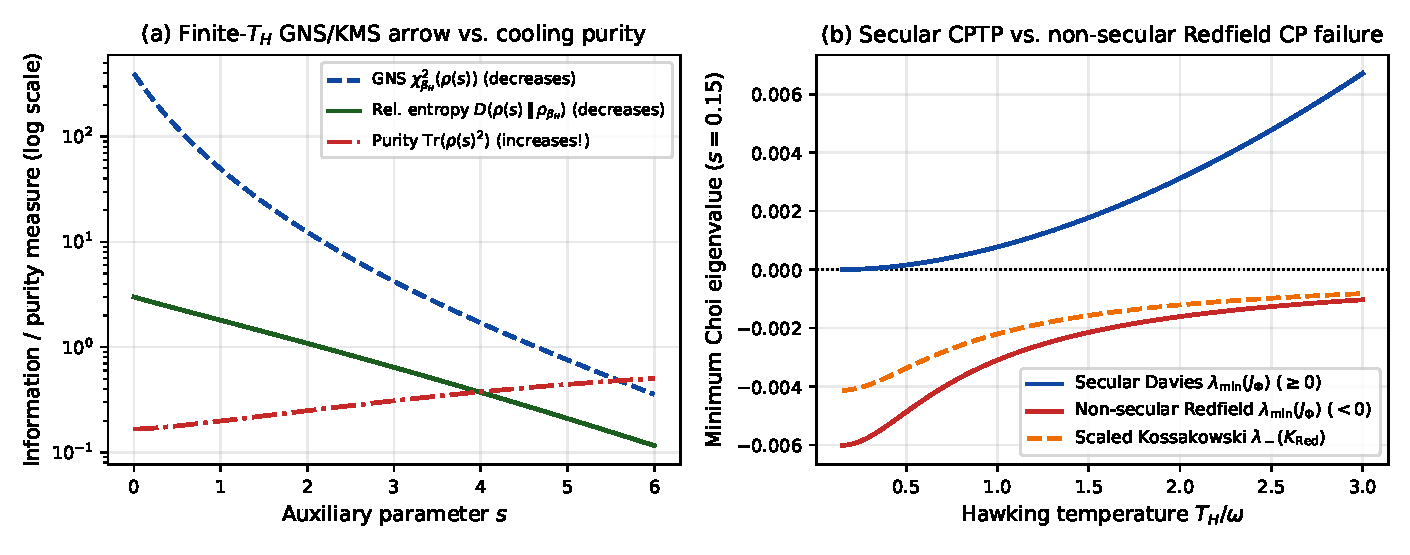
\includegraphics[width=\linewidth]{figures/fig1_covariant_kms_and_redfield.pdf}
  \caption{Theorem~\ref{thm:covariant-kms} and numerical audits F1--F2 (\code{scripts/verify\_paper2\_sk\_jt.py}). (a)~Diagonal thermal cooling of a maximally mixed $d=6$ harmonic mode ($\omega=1.2, T_H=0.65$) on a fixed-$T_H$ background: purity $\Tr(\rho(s)^2)$ increases strictly ($0.1667\to 0.5048$) while both $D(\rho(s)\|\rho_{\beta_H})$ and GNS $\chi^2_{\beta_H}(\rho(s))$ decrease monotonically (monotonicity is likewise verified in F2 for a non-commuting coherent initial state). (b)~Minimum Choi eigenvalue at $s=0.15$ vs.\ $T_H/\omega$: secular Davies evolution remains CPTP ($\lambda_{\min}\ge 0$), whereas the unprojected two-level $\sigma_x$ Bloch--Redfield generator exhibits negative Choi eigenvalues tracking $\lambda_-(K_{\mathrm{Red}})<0$.}
  \label{fig:covariant-kms}
\end{figure}

%==============================================================================
\section{2D JT Gravity + CFT Open SK Model, Two-Tiered Ward Identity, and Beyond-Gaussian Schwarzian FDT}\label{sec:jt-sk}
%==============================================================================

We next examine two-dimensional Jackiw--Teitelboim (JT) gravity \cite{Teitelboim1983,Jackiw1985,MSY2016,MertensTuriaci2023} coupled to a 2D CFT of central charge $c$ joined to an asymptotically flat radiation bath \cite{Mertens2019,AEMM2019}:
\begin{equation}\label{eq:jt-action}
\begin{aligned}
  I_{\mathrm{JT+CFT}}[g, \Phi, \phi]
  &= \frac{\Phi_0}{16\pi G_2}\!\left(\int_M \sqrt{-g}\,R + 2\int_{\partial M}\!\sqrt{-h}\,K\right) \\
  &\quad + \frac{1}{16\pi G_2}\!\left(\int_M \sqrt{-g}\,\Phi(R + 2) + 2\int_{\partial M}\!\sqrt{-h}\,\Phi(K-1)\right)
  + I_{\mathrm{CFT}}[g,\phi],
\end{aligned}
\end{equation}
with $\mathrm{AdS}_2$ length $\ell=1$. Integrating out the bulk dilaton $\Phi$ reduces the gravitational dynamics to the boundary clock reparametrization $f(u)$ governed by the Schwarzian action $I_{\mathrm{Schw}}[f] = -C\int du\,\{f(u), u\}$, $C := \Phi_b/(8\pi G_2)$ \cite{MSY2016}. In the leading large-$CT_H$ semiclassical saddle approximation, the ADM energy, Bekenstein--Hawking entropy, and heat capacity are
\begin{equation}\label{eq:jt-thermo}
  E_{\mathrm{BH}}(T_H) = 2\pi^2 C T_H^2, \qquad
  S_{\mathrm{BH}}(T_H) = S_0 + 4\pi^2 C T_H, \qquad
  C_V(T_H) = \frac{dE_{\mathrm{BH}}}{dT_H} = 4\pi^2 C T_H,
\end{equation}
where $S_0 = \Phi_0/(4G_2)$ is the extremal entropy.

\paragraph{Relation to prior SK--Schwarzian and CFT full-counting-statistics literature.}
Three established results directly overlap this section and must be attributed explicitly before identifying our additions:
(i)~The unidirectional chiral 2D CFT long-time energy-transfer cumulant generating function (CGF) and exchange fluctuation relation were derived by Bernard and Doyon \cite{BernardDoyon2012} (Eqs.~(2)--(3)) and \cite{BernardDoyon2015} (\S6.2, Prop.~6.1, Eqs.~(62)--(63), with complex-temperature shift relation Eq.~(75)):
\begin{equation}\label{eq:bd-cgf}
  \mathcal{K}_{\mathrm{BD}}(z;\beta) \;=\; \frac{\pi c}{12}\!\left(\frac{1}{\beta - z} - \frac{1}{\beta}\right)
  \;=\; \frac{\pi c}{12}\sum_{n=1}^\infty T^{n+1} z^n \qquad (T=\beta^{-1}),
\end{equation}
yielding $\mathcal{K}_{\mathrm{BD}}'(0)=\frac{\pi c}{12}T^2$, $\mathcal{K}_{\mathrm{BD}}''(0)=\frac{\pi c}{6}T^3$, and $\mathcal{K}_{\mathrm{BD}}^{(n)}(0)=\frac{\pi c}{12}\,n!\,T^{n+1}$ ($n\ge 1$). Thus our mean Hawking flux and white-noise spectral density $S_{F,\mathrm{chiral}}=\frac{\pi c}{6}T_H^3$ are inherited directly from \cite{BernardDoyon2012,BernardDoyon2015}; describing them as ``parameter-free'' means fixed by $(c,G_2,\Phi_b)$ under transparent boundary conditions, not newly discovered here.
(ii)~A microscopic Feynman--Vernon influence functional and nonlocal stochastic Schwarzian Langevin equation for 2D black-hole evaporation (including linearization around the evaporating saddle) were constructed from SYK coupled to a free-scalar bath by Gaikwad, Kaushal, Mandal, and Wadia \cite{Gaikwad2023} (\S\S3.1--3.3, Eqs.~(43), (49)--(59)), while Wilson-Gerow, Dugad, and Chen \cite{WilsonGerow2024} (\S\S II, V--VI) derived microscopic influence-functional horizon decoherence for probes near warm horizons. By contrast, \eqref{eq:jt-sk-action} below is a schematic coarse-grained decomposition taking whitening, independent increments, and a transparent junction as explicit model inputs; inserting the stationary long-time CGF \eqref{eq:bd-cgf} into time-dependent JT dynamics requires a Markovian coarse-graining window $\tau_{\mathrm{bath}} \ll \Delta u \ll \gamma_E^{-1}$ where the thermal bath correlation time scales as $\tau_{\mathrm{bath}}\sim T^{-1}$ (at $u=0$ in Test~F3, $\gamma_E/T_0 = 0.0265 \ll 1$). Our specific additions are the two-tiered Ward diffusion counterexample, the closed-form cumulant hierarchy $K_n(u)$ ($n\ge 2$) of the linearized-drift, saddle-frozen additive closure audited by zero time-discretization bias compound-Poisson Monte Carlo, the quantitative three-tier equilibrium closure comparison up to $n=4$ ($K_4/\kappa_4^{\mathrm{can}}=0.5, 1.5, 1.0$) with the explicit rational factorization of $\mathcal{H}_{\mathrm{KM}}(E,p)$, and the separation of naive finite-$q$ detailed-balance violation from a constructive $E\ge 0$ entropy-difference jump process in Proposition~\ref{prop:jt-nongaussian}.

\paragraph{What the exterior SK effective action specifies vs.\ explicit model input.}
Doubling the boundary clock and exterior CFT fields gives the schematic decomposition
\begin{equation}\label{eq:jt-sk-action}
  S_{\mathrm{SK}}^{(B)}[f_\pm, \phi_{B,\pm}] = I_{\mathrm{Schw}}[f_+] - I_{\mathrm{Schw}}[f_-] + I_{\mathrm{CFT},B}[\phi_{B,+}] - I_{\mathrm{CFT},B}[\phi_{B,-}] + S_{\mathrm{IF}}^{(B)}.
\end{equation}
Careful separation is essential between three distinct ingredients:
\begin{enumerate}
  \item \emph{Gravitational backreaction and chiral flux noise (fixed by $c, G_2, \Phi_b$):} Under transparent boundary conditions ($\cT=1$) coupling the JT boundary to a 2D CFT bath, the Bernard--Doyon first and second cumulants \cite{BernardDoyon2012,BernardDoyon2015}
  \begin{equation}\label{eq:chiral-noise}
    \langle F_{\mathrm{Hawking}}\rangle = \frac{\pi c}{12}T_H^2, \qquad
    S_{F,\mathrm{chiral}}(T_H)
    = \int_0^\infty\!\frac{d\omega}{2\pi}\,\omega^2 c\,n_{\mathrm{BE}}(\omega/T_H)\bigl(1 + n_{\mathrm{BE}}(\omega/T_H)\bigr)
    = \frac{\pi c}{6}\,T_H^3
  \end{equation}
  determine the semiclassical relaxation rate $\gamma_E = cG_2/(3\Phi_b)$ \cite{Mertens2019} and zero-frequency flux-noise amplitude without extra free coupling constants.
  \item \emph{Concrete microscopic matter-sector coupling on the outgoing Unruh sector:} Absolute matter-sector GKSL rates are \emph{not} consequences of \eqref{eq:jt-sk-action} alone; they require specifying the bath operator, sector, and coupling constant $g$. For an explicit model in which a localized exterior system operator $\mathcal{O}$ couples via $H_{\mathrm{int}} = g\,\mathcal{O}\otimes J_R(u)$ strictly to the \emph{outgoing} horizon-origin canonical free chiral boson current $J_R = \partial_u\phi_R$ in the Unruh state, whose vacuum two-point kernel is $W_J(t) = -[4\pi(t-i0^+) ^2]^{-1}$ (consistent with \eqref{eq:unruh-current}) and whose thermal outgoing kernel is $W_R(u) = -\frac{\kappa^2}{16\pi\sinh^2[\kappa(u-i0^+)/2]}$, transforming with the Fourier convention $G^>(\omega) = \int_{-\infty}^\infty dt\,e^{i\omega t}W_R(t)$ (matching the inverse measure $\frac{d\omega}{2\pi}$ in \eqref{eq:fv-quad}) yields \cite{JuarezAubryLouko2014}
  \begin{equation}\label{eq:chiral-current-rates}
    G_R^>(\omega) = \frac{\omega}{2}\bigl(1 + n_{\mathrm{BE}}(\omega/T_H)\bigr), \qquad
    G_R^<(\omega) = \frac{\omega}{2}\,n_{\mathrm{BE}}(\omega/T_H), \qquad
    \rho_{\mathrm{spec}}(\omega) = \frac{\omega}{2} \quad (\omega > 0),
  \end{equation}
  and hence $\gamma_\downarrow(\omega) = \frac{g^2\omega}{2}(1+n_{\mathrm{BE}}(\omega/T_H))$, $\gamma_\uparrow(\omega) = \frac{g^2\omega}{2}n_{\mathrm{BE}}(\omega/T_H)$ via \eqref{eq:wightman-rates} (in Test~F1, regulated numerical Fourier quadrature directly verifies the vacuum-current normalization $\int dt\,e^{i\Omega t}W_J(t)=(\Omega/2)e^{-\epsilon\Omega}$ to $1.44\times 10^{-15}$, while the thermal Bose factor $n_{\mathrm{BE}}(\omega/T_H)$ enters algebraically via KMS \eqref{eq:fdt}).
  \item \emph{Non-KMS character of the full Unruh state and exterior algebra specification:} In a general 1+1D or 3+1D Unruh state, the outgoing sector is thermal at $T_H$ while the ingoing sector from $\mathcal{I}^-$ is in its $T=0$ vacuum \cite{JuarezAubryLouko2014}. A probe coupling equally to both canonical chiral currents ($J_R$ and $J_L$) acquires $\gamma_\uparrow(\omega) = \frac{g^2\omega}{2}n_H$ and $\gamma_\downarrow(\omega) = \frac{g^2\omega}{2}(2 + n_H)$, violating single-temperature detailed balance ($\gamma_\uparrow/\gamma_\downarrow = n_H/(2+n_H) = 0.2254 \neq e^{-1} = 0.3679$ at $\beta_H\omega=1$; Test~F1); likewise, greybody-filtered outgoing occupations $\cT(\omega)n_H(\omega)$ are not themselves Gibbs distributions at $T_H$. Finally, identifying $\cA_B = \cA(W_B)$ requires explicitly choosing the observer worldline, causal wedge, and gravitational dressing \cite{JanaLoganayagamRangamani2020,ColinEllerin2021}.
\end{enumerate}

\begin{theorem}[Two-Tiered Composite Ward Identity, Semiclassical JT Saddle, and Linearized Stochastic Schwarzian FDT]\label{thm:jt-sk}
\leavevmode
\begin{enumerate}
  \item[(a)] \emph{(Two-tiered composite energy Ward identity and diffusion counterexample)} On any finite-dimensional composite system with bare additive Hamiltonian $H_{\mathrm{tot}} = H_{\mathrm{BH}} + H_{\mathrm{rad}}$ (distinct from an interacting total Hamiltonian $H_{\mathrm{BH}}+H_{\mathrm{rad}}+H_{\mathrm{int}}$ in a microscopic coupling model):
  \begin{enumerate}
    \item[(i)] \emph{(Mean energy conservation $\implies$ flux balance only)} Whenever $\cL_{\mathrm{tot}}^\dagger(H_{\mathrm{BH}}+H_{\mathrm{rad}}) = 0$, the subsystem energy fluxes balance identically: $\cL_{\mathrm{tot}}^\dagger(H_{\mathrm{BH}}) = -\cL_{\mathrm{tot}}^\dagger(H_{\mathrm{rad}})$.
    \item[(ii)] \emph{(Commuting jumps $\implies$ zero drift and zero diffusion)} Whenever every composite jump commutes with $H_{\mathrm{tot}}$ ($[H_{\mathrm{tot}}, L_k] = 0$, or equivalently both $\cL_{\mathrm{tot}}^\dagger(H_{\mathrm{tot}})=0$ and $\cL_{\mathrm{tot}}^\dagger(H_{\mathrm{tot}}^2)=0$), both the drift and total carr\'e du champ vanish: $\cL_{\mathrm{tot}}^\dagger(H_{\mathrm{tot}})=0$ and $\Gamma_{\cL_{\mathrm{tot}}}(H_{\mathrm{tot}}, H_{\mathrm{tot}}) = 0$.
    \item[(iii)] \emph{(Strict separation via 3-level counterexample)} Mean conservation alone does \emph{not} imply zero diffusion: on $\bbC^3$ with $H_3 = \mathrm{diag}(0,1,2)$ and unit-rate jumps $L_- = |0\rangle\langle 1|$, $L_+ = |2\rangle\langle 1|$ (embeddable trivially into $\bbC^3\otimes\bbC^2$ as $L_\pm\otimes\1$), $\cL^\dagger(H_3) = 0$ identically, yet $\Gamma_\cL(H_3,H_3) = 2|1\rangle\langle 1| \neq 0$ (producing $\mathrm{Var}(H_3)_s = 1 - e^{-2s} > 0$ from $|1\rangle\langle 1|$).
  \end{enumerate}
  \item[(b)] \emph{(Semiclassical evaporating 2D JT + CFT saddle \cite{Mertens2019})} For $C > 0$, $c > 0$, and initial temperature $T_0 > 0$ radiating into a $T_{\mathrm{bath}}=0$ vacuum bath, define
  \begin{equation}\label{eq:jt-rates}
    k_{\mathrm{JT}} := \frac{c}{48\pi C} = \frac{c G_2}{6\Phi_b}, \qquad
    \gamma_E := 2 k_{\mathrm{JT}} = \frac{c}{24\pi C} = \frac{c G_2}{3\Phi_b}.
  \end{equation}
  Then $T_H(u) = T_0 e^{-k_{\mathrm{JT}} u}$, $E_{\mathrm{BH}}(u) = 2\pi^2 C T_H(u)^2 = E_0 e^{-\gamma_E u}$, $S_{\mathrm{BH}}(u) = S_0 + 4\pi^2 C T_H(u)$, and the integrated thermal outgoing radiation entropy flux $S_{\mathrm{Hawking}}(u) := \int_0^u \frac{\pi c}{6}T_H(v)\,dv = 8\pi^2 C T_0 (1 - e^{-k_{\mathrm{JT}}u}) = 2(S_{\mathrm{BH}}(0) - S_{\mathrm{BH}}(u))$ solve identically:
  \begin{equation}\label{eq:jt-ward-ode}
    \frac{dE_{\mathrm{BH}}}{du} = -\frac{\pi c}{12} T_H(u)^2 = T_H(u)\frac{dS_{\mathrm{BH}}}{du}, \qquad
    \frac{dS_{\mathrm{Hawking}}}{du} = \frac{\pi c}{6} T_H(u) = -2\frac{dS_{\mathrm{BH}}}{du}.
  \end{equation}
  \item[(c)] \emph{(Linearized Gaussian white-noise stochastic Schwarzian model)}
  \begin{enumerate}
    \item[(i)] \emph{(Leading-order equilibrium FDT)} Coupled in equilibrium to a bath at $T_{\mathrm{bath}} = T_0$ under the semiclassical thermodynamics \eqref{eq:jt-thermo}, the net flux $F_{\mathrm{net}} = \frac{\pi c}{12}(T^2 - T_0^2) = \gamma_E(E - E_0)$ is linear in $E$, and two independent chiral channels yield white-noise strength $S_{\mathrm{eq}} = 2 S_{F,\mathrm{chiral}}(T_0) = \frac{\pi c}{3}T_0^3$. The resulting stationary Langevin variance matches the \emph{leading large-$CT_0$ semiclassical} canonical variance with exact factor unity:
    \begin{equation}\label{eq:jt-eq-fdt}
      \mathrm{Var}_{\mathrm{eq}}^{\mathrm{lin}}(E) \;=\; \frac{S_{\mathrm{eq}}}{2\gamma_E} \;=\; 4\pi^2 C T_0^3 \;=\; T_0^2 C_V(T_0).
    \end{equation}
    (By contrast, the fixed-topology 1-loop exact Schwarzian disk partition function $Z(\beta)\propto \beta^{-3/2}e^{S_0+2\pi^2 C/\beta}$ \cite{StanfordWitten2017} gives $\langle E\rangle = 2\pi^2 C T^2 + \frac{3}{2}T$ and $\mathrm{Var}_{\mathrm{disk}}(E) = 4\pi^2 C T^3 + \frac{3}{2}T^2$, differing by the subleading $\mathcal{O}((CT)^{-1})$ quantum correction $\frac{3}{2}T^2$.)
    \item[(ii)] \emph{(Closed-form linearized evaporating variance and multiple validity indicators)} Linearizing around the deterministic trajectory $T_H(u)$ with single-channel outgoing white noise $S_{F,\mathrm{chiral}}(T_H(u)) = \frac{\pi c}{6}T_H(u)^3$, the Gaussian variance ODE $\frac{dV}{du} = -2\gamma_E V + \frac{\pi c}{6}T_H(u)^3$ with $V(0)=0$ admits the exact non-negative solution
    \begin{equation}\label{eq:jt-evap-var}
      V(u) \;=\; 8\pi^2 C T_H(u)^3 \bigl(1 - e^{-k_{\mathrm{JT}} u}\bigr) \;\ge\; 0 \qquad (u \ge 0).
    \end{equation}
    The validity of this semiclassical, adiabatic, linearized-noise description is controlled by \emph{three distinct indicators}:
    \begin{equation}\label{eq:jt-indicators}
      C T_H(u) \gg 1, \qquad
      \epsilon_{\mathrm{ad}}(u) := \frac{k_{\mathrm{JT}}}{T_H(u)} \ll 1, \qquad
      \frac{\sqrt{V(u)}}{E_{\mathrm{BH}}(u)} = \sqrt{\frac{2(1-e^{-k_{\mathrm{JT}}u})}{\pi^2 C T_H(u)}} \ll 1.
    \end{equation}
    In particular, $\sqrt{V}/E_{\mathrm{BH}}$ reaches unity at $T_{\mathrm{fluc}} = \frac{2 T_0}{\pi^2 C T_0 + 2} \approx \frac{2}{\pi^2 C}$, roughly four times higher than the characteristic strong-coupling Schwarzian scale $T_{\mathrm{break}} := (2\pi^2 C)^{-1} = 4G_2/(\pi\Phi_b)$. Values beyond $CT_H\lesssim 1$ represent formal extrapolations of the linearized model rather than uniformly controlled semiclassical predictions.
  \end{enumerate}
\end{enumerate}
\end{theorem}

\begin{proof}
All algebraic, counterexample, and \code{HasDerivAt} statements of parts~(a)--(c) are proved directly and formalized in \code{OSTQD\_\allowbreak SK/\allowbreak Theorem2\_\allowbreak WardAndFDT.lean} (\code{bipartite\_\allowbreak energy\_\allowbreak ward\_\allowbreak identity}, \code{bipartite\_\allowbreak ward\_\allowbreak from\_\allowbreak commuting\_\allowbreak jumps}, \code{mean\_\allowbreak energy\_\allowbreak conservation\_\allowbreak nonzero\_\allowbreak diffusion}, \code{jt\_\allowbreak evaporation\_\allowbreak ward\_\allowbreak ode}, \code{jt\_\allowbreak equilibrium\_\allowbreak fdt\_\allowbreak exact}, \code{jt\_\allowbreak evaporating\_\allowbreak variance\_\allowbreak ode}). Note that \eqref{eq:jt-evap-var} assumes Markovian white-noise replacement of the zero-frequency flux noise $S_F(0)$ and linearization around the deterministic saddle; nonlinear state-dependent noise ($\mathbb{E}[T(E)^3]\neq T(\mathbb{E}[E])^3$) and finite bath-correlation times lie outside this Gaussian closure.
\end{proof}

\begin{proposition}[Frozen-Coefficient Bernard--Doyon JT Cumulants, Three-Tier Equilibrium Closure Comparison, and Constructive $E\ge 0$ Detailed-Balance Jump Process]\label{prop:jt-nongaussian}
Retaining all cumulant orders $n\ge 2$ of the coarse-grained long-time Bernard--Doyon CFT energy-transfer CGF \eqref{eq:bd-cgf} ($\kappa_n^{\mathrm{out}}(T) = \frac{\pi c}{12}\,n!\,T^{n+1}$) on the 2D JT saddle \eqref{eq:jt-thermo} (within the Markovian window $\tau_{\mathrm{bath}}\sim T^{-1} \ll \Delta u \ll \gamma_E^{-1}$) yields exact closed-form cumulants within the linearized-drift, saddle-frozen additive closure, quantitative equilibrium moment comparisons up to $n=4$ with a rational local Kramers--Moyal Hamiltonian, and an explicit stochastic jump-process completion on $E\ge 0$:
\begin{enumerate}
  \item[(a)] \emph{(Closed-form evaporating cumulants for the frozen-coefficient additive closure and state-dependent feedback contrast)} Under linearized drift and centered additive outgoing emission,
  \begin{equation}\label{eq:jt-centered-sde}
    d\,\delta E \;=\; -\gamma_E\,\delta E\,du \;-\; \Bigl[dQ_{\mathrm{out}} - \tfrac{\pi c}{12}T_H(u)^2\,du\Bigr],
  \end{equation}
  where the positive emission driver $dQ_{\mathrm{out}}$ carries saddle-frozen cumulant rates $q_n(u) := \alpha\,n!\,T_H(u)^{n+1} > 0$ ($\alpha := \frac{\pi c}{12}$), so that for every $n\ge 2$ the signed cumulant injection rate into $\delta E$ from the centered forcing $-[dQ_{\mathrm{out}} - \alpha T_H(u)^2\,du]$ is $\kappa_n^{\mathrm{inj}}(u) := (-1)^n q_n(u)$ (with vanishing first cumulant $\kappa_1^{\mathrm{inj}}=0$), the cumulant ODE $\frac{dK_n}{du} + n\gamma_E K_n = \kappa_n^{\mathrm{inj}}(u)$ ($K_n(0)=0$) admits the exact closed-form solution for every $n\ge 2$:
  \begin{equation}\label{eq:jt-kn}
    K_n(u) \;=\; (-1)^n \frac{n!}{n-1}\,4\pi^2 C\,T_H(u)^{n+1}\bigl(1 - e^{-(n-1)k_{\mathrm{JT}}u}\bigr).
  \end{equation}
  In particular, $K_2(u)=V(u)$ recovers \eqref{eq:jt-evap-var}, while the third and fourth cumulants
  \begin{equation}\label{eq:jt-k3-k4}
    K_3(u) = -12\pi^2 C T_H(u)^4\bigl(1 - e^{-2k_{\mathrm{JT}}u}\bigr) \le 0, \qquad
    K_4(u) = 32\pi^2 C T_H(u)^5\bigl(1 - e^{-3k_{\mathrm{JT}}u}\bigr) \ge 0
  \end{equation}
  yield at $2\pi^2 C T_H(u)=1$ (setting $r := T_H(u)/T_0 = e^{-k_{\mathrm{JT}}u}$) the formal frozen-model values $\gamma_1(u) = K_3/K_2^{3/2} = -\frac{3}{4}\frac{1+r}{\sqrt{1-r}}$ and $\gamma_2(u) = K_4/K_2^2 = \frac{1+r+r^2}{1-r}$, approaching $-\frac{3}{4}$ and $+1$ for $r\ll 1$ as a formal extrapolation diagnostic at $T_{\mathrm{break}}=(2\pi^2 C)^{-1}$. Because $\mathcal{K}_{\mathrm{BD}}(z;T)=\frac{\pi c T}{12}(\frac{\beta}{\beta-z}-1)$, $dQ_{\mathrm{out}}$ in \eqref{eq:jt-centered-sde} is represented identically by an independent-increment non-homogeneous compound-Poisson process with rate $\lambda(u)=\frac{\pi c}{12}T_H(u)$ and exponential jumps $J\sim\mathrm{Exp}(\text{mean }T_H(u))$ (an exact representation of the frozen-coefficient Markov CGF driver, not literal microscopic memoryless jumps; the linearly filtered fluctuation $\delta E$ does not have independent increments). Crucially, the negative skewness in \eqref{eq:jt-k3-k4} is specific to this frozen-coefficient closure rather than a universal leading prediction of state-dependent evaporating JT gravity: restoring state-dependent temperature $T(E)=\sqrt{E/A_C}$ ($A_C := 2\pi^2 C$) in the outgoing jump generator ($D_n(E)=(-1)^n\alpha n!\,T(E)^{n+1}$) yields the leading semiclassical moment ODEs $\dot{K}_2 = -2\gamma_E K_2 + 2\alpha T^3$ and $\dot{K}_3 = -3\gamma_E K_3 + 3D_2'(\bar{E})K_2 + D_3(\bar{E})$. At fixed $c, T_0, u/C$, both source terms contribute at the same leading $\mathcal{O}(C)$ order over $u=\mathcal{O}(C)$, shifting the leading state-dependent third cumulant from \eqref{eq:jt-k3-k4} to $K_3^{\mathrm{state,lead}} = 6 A_C T^4(1-r)(5-7r)$, which turns positive for $r < 5/7$ (for F3 parameters at $u=30$, frozen $K_3(30) = -158.80$ vs.\ state-dependent $K_3^{\mathrm{state,lead}}(30) = +28.29$, verified against independent ODE integration to $3.52\times 10^{-15}$).
  \item[(b)] \emph{(Primary equilibrium result: local Kramers--Moyal Hamiltonian and three-tier comparison up to $n=4$)} Compare the leading large-$CT_0$ canonical Gibbs cumulants $\kappa_n^{\mathrm{can}} = n!\,2\pi^2 C T_0^{n+1}$, obtained from $(-1)^n\partial_\beta^n(2\pi^2 C/\beta)$ ($\kappa_2^{\mathrm{can}}=4\pi^2 C T_0^3$, $\kappa_3^{\mathrm{can}}=+12\pi^2 C T_0^4$, $\kappa_4^{\mathrm{can}}=+48\pi^2 C T_0^5$), against three specific open-system closures sharing the fixed Bernard--Doyon drift and noise coefficients when coupled to a bath at $T_0=\beta_0^{-1}$:
  \begin{enumerate}
    \item[(i)] \emph{Tier~1 (linearized additive two-channel Bernard--Doyon noise):} Matches $\kappa_2^{\mathrm{can}}$, but strictly fails at $n=3$ and $n=4$: $K_3^{\mathrm{lin,eq}} = 0 \neq \kappa_3^{\mathrm{can}}$ and $K_4^{\mathrm{lin,eq}} = 24\pi^2 C T_0^5 = \frac{1}{2}\kappa_4^{\mathrm{can}} \neq \kappa_4^{\mathrm{can}}$.
    \item[(ii)] \emph{Tier~2 (purely Gaussian state-dependent diffusion $D_2(E)=\frac{\pi c}{6}[T(E)^3+T_0^3]$ with fixed BD drift):} Retaining multiplicative temperature dependence $T(E)=\sqrt{E/(2\pi^2 C)}$ ($D_2'(E_0)=3\gamma_E T_0$, $D_2''(E_0)=3\gamma_E T_0/(2E_0)$) while truncating the Kramers--Moyal expansion at $k=2$ repairs the third cumulant ($K_3^{\mathrm{Gauss,eq}}=+12\pi^2 C T_0^4=\kappa_3^{\mathrm{can}}$), yet \emph{overshoots the fourth cumulant by $50\%$}: $K_4^{\mathrm{Gauss,eq}} = (6 D_2'(E_0)\kappa_3^{\mathrm{can}} + 6 D_2''(E_0)(\kappa_2^{\mathrm{can}})^2)/(4\gamma_E) = +72\pi^2 C T_0^5 = \frac{3}{2}\kappa_4^{\mathrm{can}} \neq \kappa_4^{\mathrm{can}}$. (This obstruction compares closures keeping the fixed Bernard--Doyon drift; it does not rule out a separate Gaussian Fokker--Planck model whose drift is modified to $b(E)=\frac{1}{2}D'(E)+\frac{1}{2}D(E)\psi'(E)$ with $\psi(E):=S_{\mathrm{BH}}(E)-\beta_0 E$.)
    \item[(iii)] \emph{Tier~3 (local state-dependent Bernard--Doyon Kramers--Moyal Hamiltonian and $n=4$ cancellation):} Retaining both state-dependent temperature $\beta(E)=T(E)^{-1}=S_{\mathrm{BH}}'(E)$ and non-Gaussian cumulants yields the local large-deviation Kramers--Moyal Hamiltonian $\mathcal{H}_{\mathrm{KM}}(E,p) := \mathcal{K}_{\mathrm{BD}}(-p; T(E)) + \mathcal{K}_{\mathrm{BD}}(+p; T_0)$, which obeys the Bernard--Doyon exchange fluctuation symmetry $\mathcal{H}_{\mathrm{KM}}(E,p)=\mathcal{H}_{\mathrm{KM}}(E,\beta_0-\beta(E)-p)$ \cite{BernardDoyon2012,BernardDoyon2015} and \emph{factors rationally} for all $E>0$ as
    \begin{equation}\label{eq:hj-factor}
      \mathcal{H}_{\mathrm{KM}}(E,p)
      \;=\; \frac{\pi c}{12}\,\frac{p\,\bigl(\beta(E)+\beta_0\bigr)\,\bigl(p - [\beta_0 - \beta(E)]\bigr)}{\beta_0\,\beta(E)\,(\beta_0 - p)\,(\beta(E) + p)}.
    \end{equation}
    On its real-CGF strip $-\beta(E) < p < \beta_0$, \eqref{eq:hj-factor} vanishes identically along the canonical slope $p = \beta_0 - \beta(E) = V'(E) = -\psi'(E)$, where $\psi(E) := S_{\mathrm{BH}}(E)-\beta_0 E$ and $V(E) := (\sqrt{E}-\sqrt{E_0})^2/T_0 \ge 0$ is the non-negative Freidlin--Wentzell quasipotential. At $n=4$, adding $D_3'(E_0)=-12\gamma_E T_0^2$ and $D_4(E_0)=4\pi c T_0^5$ cancels the $50\%$ Tier-2 Gaussian overshoot identically ($54+18-48+24 = 48$), restoring $K_4^{\mathrm{KM,eq}} = 48\pi^2 C T_0^5 = \kappa_4^{\mathrm{can}}$ at leading large-$CT_0$ order.
  \end{enumerate}
  \item[(c)] \emph{(Finite-$q$ detailed-balance obstruction for naive rates vs.\ constructive $E\ge 0$ entropy-difference jump process)} Crucially, the local zero-locus $\mathcal{H}_{\mathrm{KM}}(E,V'(E))=0$ does \emph{not} by itself define a reversible Markov jump process on $E\ge 0$ or establish all-order stationary cumulant convergence without specifying boundary conditions and large-$C$ scaling. Indeed, adopting the naive state-dependent Bernard--Doyon jump-rate densities $w_-^{\mathrm{naive}}(E,q)=\alpha e^{-q\beta(E)}$ and $w_+(E,q)=\alpha e^{-q\beta_0}$ ($\alpha=\frac{\pi c}{12}$) fails on two counts: (i)~allowing $q>E$ exits the physical domain $E\ge 0$; (ii)~even rejecting $q>E$, strict concavity of $S_{\mathrm{BH}}(E)=2\pi\sqrt{2CE}$ enforces for all $C,E,q>0$ the strict inequality
  \begin{equation}\label{eq:naive-db-obstruction}
    q\beta(E+q) \;<\; S_{\mathrm{BH}}(E+q) - S_{\mathrm{BH}}(E) \;<\; q\beta(E),
  \end{equation}
  so $\ln[w_+(E,q)/w_-^{\mathrm{naive}}(E+q,q)] = q[\beta(E+q)-\beta_0] \neq [S_{\mathrm{BH}}(E+q)-S_{\mathrm{BH}}(E)]-\beta_0 q$, strictly violating exact finite-$q$ detailed balance for the classical canonical weight $\pi(E)\propto e^{S_{\mathrm{BH}}(E)-\beta_0 E}$ (formalized in \code{jt\_\allowbreak naive\_\allowbreak bd\_\allowbreak finite\_\allowbreak q\_\allowbreak detailed\_\allowbreak balance\_\allowbreak obstruction}). By contrast, replacing the emission rate density on $E\ge 0$ with the \emph{entropy-difference jump kernel}---whose $e^{S(E-q)-S(E)}$ emission exponent follows the backreaction / Hawking-tunneling structure of Massar--Parentani \cite{MassarParentani2000} and Parikh--Wilczek \cite{ParikhWilczek2000} (Eq.~(10)), combined here with the JT entropy and specified incoming rate $w_+$ into a reversible $E\ge 0$ jump process compared against Bernard--Doyon \cite{BernardDoyon2015} (Prop.~6.1, Eqs.~(62)--(63))---
  \begin{equation}\label{eq:ediff-jump-kernel}
    w_-(E,q) := \begin{cases}\alpha\,e^{S_{\mathrm{BH}}(E-q)-S_{\mathrm{BH}}(E)}, & 0 < q \le E, \\ 0, & q > E,\end{cases}
    \qquad
    w_+(E,q) := \alpha\,e^{-q\beta_0} \quad (q>0)
  \end{equation}
  defines a \emph{non-explosive} Markov jump process confined to $E\ge 0$: incoming jumps form a compound Poisson process of rate $\alpha/\beta_0$ whose cumulative jump sum on any $[0,T]$ is almost surely finite (yielding an a.s.\ finite upper bound on $E(u)$ over $[0,T]$), and by monotonicity of $S_{\mathrm{BH}}$, the total emission rate obeys $\int_0^E w_-(E,q)\,dq \le \alpha E$, ruling out infinitely many emissions in finite time. The kernel \eqref{eq:ediff-jump-kernel} satisfies \emph{exact finite-$q$ detailed balance} $\pi(E)w_+(E,q) = \pi(E+q)w_-(E+q,q)$ for all $E\ge 0, q>0$ and reproduces the Bernard--Doyon emission rate in the large-$C$ scaling $E=Ce$ ($q=\mathcal{O}(T)$) with first curvature correction $\frac{1}{2}S_{\mathrm{BH}}''(E)q^2 = -\frac{\beta(E)}{4E}q^2 < 0$. Moreover, writing $A := 2\pi^2 C$ and omitting the cancelling constant $S_0$, the stationary partition function of the weight $e^{2\sqrt{AE}-\beta E}\,dE$ on $E\ge 0$ evaluates directly by completing the square in $\sqrt{\beta E}-\sqrt{A/\beta}$:
  \begin{equation}\label{eq:ediff-partition}
    Z_C(\beta) \;=\; \int_0^\infty e^{2\sqrt{AE}-\beta E}\,dE
    \;=\; \frac{1}{\beta} + \frac{\sqrt{\pi A}}{\beta^{3/2}}\,e^{A/\beta}\,\mathrm{erfc}\!\left(-\sqrt{\frac{A}{\beta}}\right)
    \qquad (\beta > 0).
  \end{equation}
  On a small complex neighborhood of fixed $\beta_0 = T_0^{-1} > 0$, $\ln Z_C(\beta) = A/\beta - \frac{3}{2}\ln\beta + \ln(2\sqrt{\pi A}) + \mathcal{O}(e^{-aC})$ ($a>0$), so differentiating the stationary CGF $\ln Z_C(\beta_0-z)-\ln Z_C(\beta_0)$ yields for every \emph{fixed} order $n\ge 1$ the exact large-$C$ stationary cumulant expansion
  \begin{equation}\label{eq:ediff-cumulants}
    \kappa_n \;=\; n!\,A\,T_0^{n+1} + \frac{3}{2}(n-1)!\,T_0^n + \mathcal{O}_n(e^{-aC}).
  \end{equation}
  (This establishes exact leading-order agreement with $\kappa_n^{\mathrm{can}} = n! A T_0^{n+1}$ for each fixed $n\ge 1$, without claiming uniform-in-$n$ convergence as $n\to\infty$; note also that the classical weight $e^{2\sqrt{AE}}\,dE$ differs near $E=0$ from the exact Schwarzian disk density of states $\rho_{\mathrm{disk}}(E)\propto\sinh(2\sqrt{AE})$ of \cite{StanfordWitten2017} (\S2.4, Eq.~(2.39)), while sharing the same large-$C$ saddle and one-loop $\frac{3}{2}(n-1)!T_0^n$ subleading terms up to $\mathcal{O}_n(e^{-aC})$.)
\end{enumerate}
\end{proposition}

\begin{proof}
Matching Table~\ref{tab:lean}'s formalization boundary, \code{OSTQD\_\allowbreak SK/\allowbreak Theorem2\_\allowbreak WardAndFDT.lean} (11 public declarations total for Theorem~\ref{thm:jt-sk} and Proposition~\ref{prop:jt-nongaussian}) machine-checks the $n=3,4$ frozen-coefficient evaporating ODEs and signs \eqref{eq:jt-k3-k4}, the Tier~1/Tier~2 equilibrium ratios, the rational factorization \eqref{eq:hj-factor}, its vanishing at $p=\beta_0-\beta(E)$, the leading fourth-cumulant cancellation, the strict finite-$q$ detailed-balance obstruction \eqref{eq:naive-db-obstruction}, and the finite-$q$ detailed balance, boundary confinement, and exact \code{HasDerivAt} entropy derivatives $S_{\mathrm{BH}}'(E)=\beta(E)$, $S_{\mathrm{BH}}''(E)=-\beta(E)/(2E)<0$ of \eqref{eq:ediff-jump-kernel}. Pathwise non-explosion of \eqref{eq:ediff-jump-kernel}, direct Gaussian integration of $Z_C(\beta)$ in \eqref{eq:ediff-partition}, and fixed-$n$ stationary cumulant asymptotics \eqref{eq:ediff-cumulants} belong to the analytical proof above (with a test-function generator-integral stationarity check and $Z_C(\beta)$ / $\kappa_n$ quadrature audited in Test~F3). Subleading $\mathcal{O}((CT_0)^{-1})$ 1-loop Schwarzian disk corrections \cite{StanfordWitten2017} and finite bath-correlation times \cite{Gaikwad2023} remain distinct from this Markovian leading-order closure.
\end{proof}

\begin{remark}[Epistemic scope: Layer~1 open dynamics vs.\ Layer~2 actualization]\label{rem:layer12}
The semiclassical JT + CFT analysis yields Layer~1 reduced open-system dynamics (energy relaxation $\gamma_E$, cumulants $K_n(u)$, and equilibrium fluctuation-relation / jump-process structure \eqref{eq:hj-factor}--\eqref{eq:ediff-cumulants}) within the regime \eqref{eq:jt-indicators} and Markovian window $\tau_{\mathrm{bath}}\ll\Delta u\ll\gamma_E^{-1}$; it does \emph{not} derive intrinsic Layer~2 single-shot actualization (Remark~\ref{rem:layer2-gauge}), nor does it resolve the strong-coupling regime $CT_H \lesssim 1$.
\end{remark}

Figure~\ref{fig:jt-fdt} displays the evaporation trajectory and all validity indicators (Test~F3, $C=12, c=24, S_0=20, T_0=1$): $CT_H = 1$ occurs at $u_{CT=1}=187.36$ ($\epsilon_{\mathrm{ad}}=0.159$, $\sqrt{V}/E_{\mathrm{BH}}=0.431$, where the formal Gaussian model assigns tail weight $P(E<0)\approx 1.02\%$, while frozen-coefficient Bernard--Doyon skewness is $\gamma_1=-0.1910$ and excess kurtosis $\gamma_2=+0.0603$), $\sqrt{V}/E_{\mathrm{BH}}=1$ at $u_{\mathrm{fluc}}=308.98$ ($T_{\mathrm{fluc}}=0.01661$), $\epsilon_{\mathrm{ad}}=1$ at $u_{\mathrm{ad}}=325.93$, and $2\pi^2 CT_H=1$ at $u_{\mathrm{break}}=412.24$ ($\epsilon_{\mathrm{ad}}=\pi$, $\sqrt{V}/E_{\mathrm{BH}}=1.996$, $\gamma_1=-0.7548$, $\gamma_2=+1.0085$); the Stanford--Witten 1-loop disk correction to $\mathrm{Var}_{\mathrm{eq}}(E)$ at $CT_0=12$ is $0.317\%$. Using the exact one-step Gaussian transition variance $Q_{\mathrm{exact}}(u_n,\Delta u) = S_* e^{-3k_{\mathrm{JT}}u_n} e^{-4k_{\mathrm{JT}}\Delta u}(e^{k_{\mathrm{JT}}\Delta u}-1)/k_{\mathrm{JT}}$ (zero time-discretization bias, \code{ddof=1}), $2\times 10^4$ Gaussian Monte Carlo trajectories match \eqref{eq:jt-evap-var} to $0.31\%$ at $u=187.57$ ($CT_H=0.997$) and $0.43\%$ at $0.65 u_{\mathrm{break}}$. Independently, continuous-time non-homogeneous compound-Poisson Monte Carlo ($10^5$ trajectories, zero time-discretization bias) for the frozen-coefficient additive closure \eqref{eq:jt-centered-sde} matches $K_2$ to $0.46\%$ and $K_3$ to $2.18\%$ at $u_{CT=1}$ (MC $\gamma_1=-0.1938$), and matches $K_2$ to $0.50\%$, $K_3$ to $0.72\%$, and $K_4$ to $0.15\%$ at $u_{\mathrm{break}}$ (MC $\gamma_1=-0.7549$, $\gamma_2=+1.0201$; note that these percentages measure finite-sample Monte Carlo error of the simulated frozen closure, whereas physical approximation errors such as state-dependent feedback $K_3^{\mathrm{state,lead}}(30)=+28.29$ vs.\ $-158.80$ are evaluated separately). Finally, Test~F3 confirms the Hamilton--Jacobi zero-locus residual $0.0$ across $E/E_0\in[0.2,3.0]$, naive finite-$q$ detailed-balance log-ratio violations up to $0.5956$ across $q\in[0.2,15]$, exact finite-$q$ detailed balance ($0.0$ residual) and large-$C$ curvature agreement ($1.06\times 10^{-4}$ at $q=0.05$) for \eqref{eq:ediff-jump-kernel}, an independent generator-integral stationarity check $\int_0^\infty\pi(E)(Lf)(E)\,dE$ for the test function $f(E)=e^{-0.1E}$ at $\alpha=1, C=0.5, \beta_0=1.2$ (incoming $-0.03019737093214$ vs.\ outgoing $+0.03019737093214$, net residual $1.89\times 10^{-15}$, contrasted with $+0.00632818$ for naive $q>E$-rejected emission), direct quadrature agreement of \eqref{eq:ediff-partition} ($6.90\times 10^{-16}$), and agreement of the $C=12, \beta_0=1$ stationary cumulants $\kappa_1,\dots,\kappa_4$ with \eqref{eq:ediff-cumulants} to max relative error $8.42\times 10^{-13}$.

\begin{figure}[!tb]
  \centering
  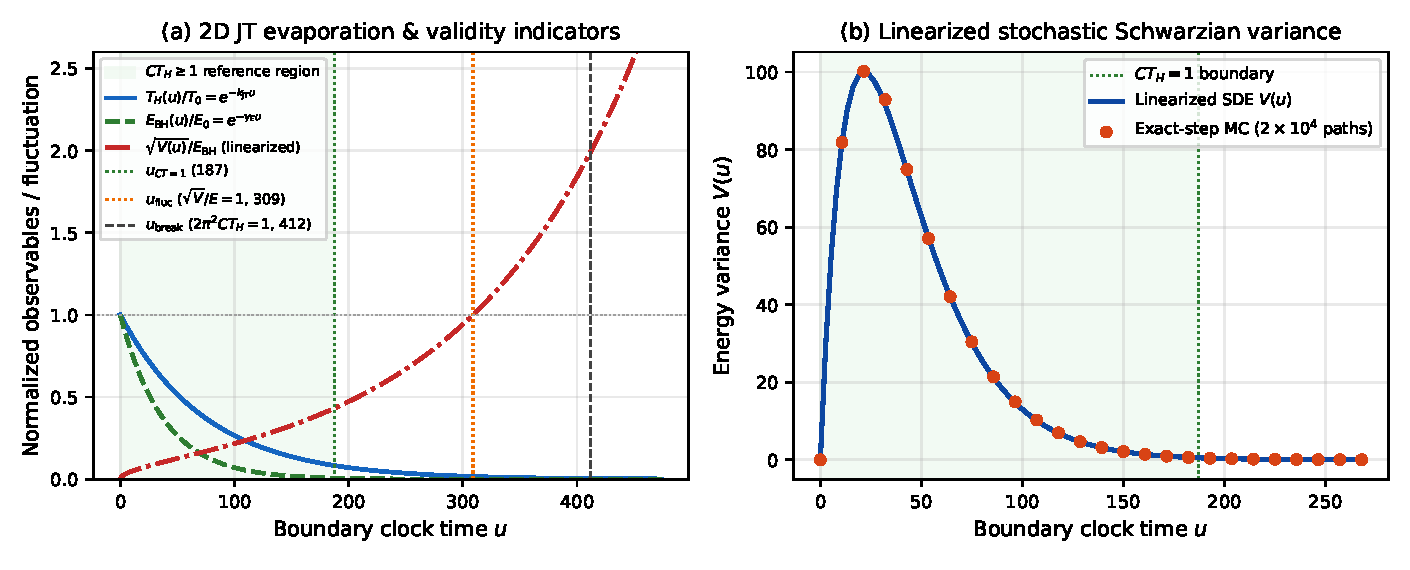
\includegraphics[width=\linewidth]{figures/fig2_jt_sk_evaporation_fdt.pdf}
  \caption{Theorem~\ref{thm:jt-sk} and numerical audit F3 ($C=12, c=24, S_0=20, T_0=1$). (a)~Semiclassical 2D JT + CFT evaporation trajectory $T_H(u)/T_0$ and $E_{\mathrm{BH}}(u)/E_0$ with the shaded $CT_H\ge 1$ reference region ($u\le 187.36$; note that uniform semiclassical control requires $CT_H\gg 1$ since $\sqrt{V}/E_{\mathrm{BH}}=0.431$ at $CT_H=1$) separated from the formal linear-model extrapolation ($u > 187.36$), marking the distinct indicators $u_{CT=1}=187.36$, $u_{\mathrm{fluc}}=308.98$ ($\sqrt{V}/E_{\mathrm{BH}}=1$), and $u_{\mathrm{break}}=412.24$ ($2\pi^2 CT_H=1$). (b)~Linearized stochastic Schwarzian variance $V(u)$ \eqref{eq:jt-evap-var} vs.\ $2\times 10^4$ exact-step Gaussian Monte Carlo paths (zero time-discretization bias; $0.31\%$ relative error at $CT_H\simeq 1$).}
  \label{fig:jt-fdt}
\end{figure}

%==============================================================================
\section{Bosonic All-\texorpdfstring{$s$}{s} Mode Law, Chiral-Horizon Smooth-Band Obstructions, and Single-Shot Firewall Floor}\label{sec:hadamard}
%==============================================================================

We next extend our preceding finite-dimensional single-mode excitation bound \cite{Soga2026OSTQD} to arbitrary bosonic Fock truncations and establish our central continuum obstruction and Mellin positive-type extension theorem for a \emph{free $c=1$ chiral boson field} (or $N_f$ decoupled free copies; interacting CFTs are not assumed here), carefully separating single-mode oscillator Hamiltonians, symmetric cross-horizon point-split diagnostics, tempered distributional contact extensions, nonlinear detectors, and single-shot selective projections \cite{ArakiShiraishi1971,KayWald1991,Radzikowski1996,LoukoSatz2008,SperlingVogel2012,MaldacenaSusskind2013,Louko2014,Sanders2015,Ho2016,Zambianco2026}.

\paragraph{Exact bosonic all-$s$ mode law and attribution to Sperling--Vogel (2012).}
In the two-mode squeezed inertial vacuum $|0_A\rangle = (\cosh r)^{-1}\sum_{n=0}^\infty (\tanh r)^n |n_R,n_L\rangle$ ($\tanh r = e^{-\omega/(2T_H)}$, $n_{\mathrm{BE}}=\sinh^2 r$), exterior-local Killing-conserving dephasing $\cL_B(\rho)=-\frac{\Gamma}{2}[N_R,[N_R,\rho]]$ preserves the Schmidt subspace $\mathrm{span}\{|n_R,n_L\rangle\}$ and produces the one-sided Gaussian phase-diffused two-mode squeezed state family
\begin{equation}\label{eq:sperling-vogel}
  \rho_s \;=\; (1-\zeta^2)\sum_{m,n\ge 0} \zeta^{m+n}\,e^{-\sigma^2(m-n)^2/2}\,|m_R,m_L\rangle\langle n_R,n_L|, \qquad
  \zeta := \tanh r,\quad \sigma^2 := \Gamma s.
\end{equation}
This density-matrix family was already derived and analyzed by Sperling and Vogel \cite{SperlingVogel2012} (\S II, Eq.~(4)); we do not claim priority over the state \eqref{eq:sperling-vogel}. Our additions are its evaluation on the squeezed-basis single-mode inertial quadratic form $H_A(\omega) = \omega[\cosh(2r)(N_R+N_L+1)-\sinh(2r)(b_R^\dagger b_L^\dagger+b_R b_L)-1]$ (distinct from the local Minkowski stress tensor and wavepacket-smeared mode Hamiltonians \cite{Bruschi2010}), an arbitrary-$N$ Lean-verified \code{HasDerivAt} ODE, the exact $\mathcal{O}(Nq^N)$ Fock truncation remainder, and the continuum horizon-diagnostic classification below. Note already at the single-mode level that the phase-averaged state \eqref{eq:sperling-vogel} is strictly non-Gaussian and distinguished at four-point order from the centered quasifree state sharing its attenuated two-point covariance $\langle b_R b_L\rangle = b\sqrt{n(n+1)}$ ($n:=\sinh^2 r$, $b:=e^{-\Gamma s/2}$): because \eqref{eq:sperling-vogel} preserves diagonal number probabilities, $\langle N_R N_L\rangle_{\mathrm{SV}} = n^2 + n(n+1)$, whereas Wick's theorem gives $\langle N_R N_L\rangle_{\mathrm{QF}} = n^2 + b^2 n(n+1)$, differing by $(1-b^2)n(n+1)$, which is strictly positive whenever $n>0$ and $\Gamma(\omega)s>0$ (vanishing at $s=0$ or outside the dephasing support where the two-mode squeezed vacuum is preserved; e.g.\ $0.42293033$ vs.\ $0.12187693$ at $T_H/\omega=0.65, \Gamma s=2$, Test~F4).

\paragraph{Continuum free 2D chiral boson kernel and comparison with closely related horizon models.}
Consider the IR-finite outgoing chiral current $J(X^-) := \partial_{X^-}\phi(X^-)$ of a free $c=1$ massless chiral boson in Kruskal coordinate $X^-\in\bbR$ (exterior wedge $W_B$: $X^-=-\kappa^{-1}e^{-\kappa u}<0$; interior $I$: $X^-=+\kappa^{-1}e^{\kappa\tilde{u}}>0$, $\kappa=2\pi T_H$). In the Unruh state $|0_A\rangle$,
\begin{equation}\label{eq:unruh-current}
  W_{\mathrm{Unruh}}(X_1^-, X_2^-) \;:=\; \langle 0_A | J(X_1^-) J(X_2^-) | 0_A \rangle \;=\; -\frac{1}{4\pi(X_1^- - X_2^- - i0^+)^2},
\end{equation}
which carries no horizon singularity beyond the universal Hadamard coincidence singularity at $X_1^-=X_2^-$ \cite{KayWald1991,Sanders2015}. Expanding $J$ in Killing modes $(b_R(\omega), b_L(\omega))$, strictly exterior points ($X_1^-, X_2^- < 0$) depend solely on diagonal exterior occupations $\langle b_R^\dagger(\omega)b_R(\omega)\rangle = n_{\mathrm{BE}}(\omega)$, whereas strictly separated cross-horizon points ($X_1^- < 0 < X_2^-$, $\sigma := \kappa^{-1}\ln(X_2^-/|X_1^-|)$) arise purely from cross-horizon entanglement $\langle b_R(\omega)b_L(\omega)\rangle = (2\sinh(\pi\omega/\kappa))^{-1}$:
\begin{equation}\label{eq:rl-integral}
  W_{RL}^{\mathrm{Unruh}}(X_1^-, X_2^-) \;=\; -\frac{1}{4\pi \kappa^2 |X_1^-| X_2^-} \int_0^\infty d\omega\,\frac{\omega\cos(\omega\sigma)}{\sinh(\pi\omega/\kappa)} \;=\; -\frac{1}{4\pi(|X_1^-| + X_2^-)^2}.
\end{equation}
Applying modewise exterior $N_{R,\omega}$-dephasing on a \emph{single global state} attenuates the integrand of \eqref{eq:rl-integral} by $e^{-\Gamma(\omega)s/2}$ at off-horizon points $X_1^- < 0 < X_2^-$ (and symmetrically for $X_2^- < 0 < X_1^-$) while leaving all strictly exterior ($R$--$R$) and strictly interior ($L$--$L$) correlators unchanged. This setup differs in three concrete respects from closely related prior models:
(i)~Maldacena--Susskind \cite{MaldacenaSusskind2013} (\S5.5, Eqs.~(5.3)--(5.5)) consider coherent phase-unitary deformations of an entangled pure state; the present $N_{R,\omega}$-dephasing instead averages over phases, and in the complete-dephasing limit ($s\to\infty$) retains classical cross-horizon number correlations $\sum_n c_n^2|n_R,n_L\rangle\langle n_R,n_L|$, in contrast to the uncorrelated thermal-product construction $\rho_R^{\mathrm{th}}\otimes\rho_L^{\mathrm{th}}$ used by Louko \cite{Louko2014} (\S4.1) (though the corresponding off-horizon two-point kernels can coincide for uniform $\Gamma_0$ even while the full states differ);
(ii)~unlike Louko's Rindler firewall model \cite{Louko2014}, which adopts a specific distributional prescription yielding a \emph{finite} derivative-coupled detector response, we analyze both the raw radial cutoff integral and arbitrary finite-order point-contact extensions supported at $(0,0)$;
(iii)~unlike Ho, Su, Mann, and Ralph's frequency-selective firewall model \cite{Ho2016} (Eqs.~(10)--(14)), which modifies occupation spectra, our $N_{R,\omega}$-dephasing preserves the exact thermal exterior marginal on every frequency mode; and unlike Wilson-Gerow, Dugad, and Chen \cite{WilsonGerow2024}, whose decoherence arises from a microscopic probe--horizon influence functional, $\Gamma(\omega)$ here is an external observer-indexed dephasing diagnostic.

\begin{theorem}[All-$s$ Bosonic Mode ODE, Free Chiral Boson Point-Split Defect, and Fixed-$s$ CPL]\label{thm:hadamard}
\leavevmode
\begin{enumerate}
  \item[(a)] \emph{(Arbitrary-$N$ bosonic all-$s$ \code{HasDerivAt} ODE and tridiagonal mode law)} For every truncation dimension $N\ge 1$, real amplitudes $c_n$, rate $\Gamma\ge 0$, and $s\in\bbR$, $\rho^{(N)}_{ij}(s) := c_i c_j e^{-\Gamma s(i-j)^2/2}$ \cite{SperlingVogel2012} solves $\frac{d}{ds}\rho^{(N)}(s) = -\frac{\Gamma}{2}[N_R,[N_R,\rho^{(N)}(s)]]$ entrywise, preserves every diagonal exterior observable $\Tr(D\rho^{(N)}(s)) = \Tr(D\rho^{(N)}(0))$, and obeys for any tridiagonal $H_A^{(N)}$:
  \begin{equation}\label{eq:tridiag-all-s}
    \Tr\bigl(H_A^{(N)}\rho^{(N)}(s)\bigr) - \Tr\bigl(H_A^{(N)}\rho^{(N)}(0)\bigr)
    = \Bigl(\Tr\bigl(H_A^{(N)}\rho^{(N)}_{\mathrm{diag}}\bigr) - \Tr\bigl(H_A^{(N)}\rho^{(N)}(0)\bigr)\Bigr)\bigl(1 - e^{-\Gamma s/2}\bigr).
  \end{equation}
  In the $N\to\infty$ Fock limit at fixed $\omega > 0$ (where the truncated expectation converges uniformly in $s\ge 0$ with exact boundary remainder $\frac{2\omega N q^N}{(1-q)(1-q^N)}[2e^{-\Gamma s/2}-(1+q)] = \mathcal{O}(N q^N)$, $q:=e^{-\beta_H\omega}$, though non-uniformly as $\omega\to 0$), this gives the exact all-$s$ single-mode excitation law ($\sigma=+1$ bosons, $\sigma=-1$ fermions):
  \begin{equation}\label{eq:unified-all-s}
    \langle H_A(\omega)\rangle_{\rho_B(s)} \;=\; 4\omega\,n_\sigma(\omega)\bigl(1 + \sigma\,n_\sigma(\omega)\bigr)\bigl(1 - e^{-\Gamma(\omega) s/2}\bigr) \qquad \forall s \ge 0.
  \end{equation}
  \item[(b)] \emph{(Free 2D chiral boson point-split non-Hadamard diagnostic and uniform-$\Gamma$ raw-cutoff UDW integral)} Under modewise off-horizon dephasing on a single global state with $s>0$ and $\Gamma\ge 0$ nonzero on a positive-measure frequency set:
  \begin{enumerate}
    \item[(i)] \emph{(Fixed-$s$ exterior invariance)} Whenever $X_1^-, X_2^- < 0$ and $s\ge 0$, one has $W_s(X_1^-, X_2^-) = W_{\mathrm{Unruh}}(X_1^-, X_2^-)$, so the $u$-normal-ordered (asymptotic Boulware $u$-vacuum subtracted) outgoing chiral flux $\langle T_{uu}(u)\rangle_{\mathrm{ren}} = +\frac{\pi}{12}T_H^2$ (per $c=1$ copy) is identically unchanged.
    \item[(ii)] \emph{(Cross-horizon $\epsilon^{-2}$ point-split non-Hadamard defect)} Across $X^-=0$ at symmetric point-splitting $(-\epsilon,+\epsilon)$,
    \begin{equation}\label{eq:hadamard-defect}
      \Delta W_J(-\epsilon, +\epsilon; s) := W_s(-\epsilon, +\epsilon) - W_{\mathrm{Unruh}}(-\epsilon, +\epsilon)
      = \frac{C_\Gamma(s)}{4\pi \kappa^2 \epsilon^2} \;\xrightarrow{\epsilon\to 0^+}\; +\infty,
    \end{equation}
    where $C_\Gamma(s) := \int_0^\infty d\omega\,\frac{\omega}{\sinh(\pi\omega/\kappa)}(1 - e^{-\Gamma(\omega)s/2}) > 0$; for uniform $\Gamma_0>0$, $C_{\Gamma_0}(s)=\frac{\kappa^2}{4}(1-e^{-\Gamma_0 s/2})$ and the point-split defect reduces to $\Delta W_J(-\epsilon,+\epsilon;s)=(1-e^{-\Gamma_0 s/2})/(16\pi\epsilon^2)$. Because any Hadamard two-point function differs from $W_{\mathrm{Unruh}}$ by a smooth function across $X^-=0$ \cite{Radzikowski1996,Sanders2015}, \eqref{eq:hadamard-defect} rules out Hadamard regularity for every extension agreeing with $W_s$ off the horizon, while demonstrating breakdown of standard point-splitting at $X^-=0$ rather than assigning a finite local stress-energy value.
    \item[(iii)] \emph{(Uniform-$\Gamma_0$ raw-cutoff UDW divergence)} Along the affine horizon-crossing trajectory $X^-(\tau) = \tau$ coupled to $J(X^-)$ (a general worldline inserts $\dot{X}^-(\tau_1)\dot{X}^-(\tau_2)$), combining both cross-horizon quadrants ($2\,\mathrm{Re}$ over $\tau_1<0<\tau_2$) with radial cutoff $r=|\tau_1|+\tau_2 \ge \epsilon_{\mathrm{UV}}$ and Gaussian switching $\chi(\tau) = e^{-\tau^2/(2\sigma_\tau^2)}$ yields for uniform $\Gamma_0>0$ the leading-order ($\mathcal{O}(g^2)$) raw-cutoff defect
    \begin{equation}\label{eq:udw-div}
      \Delta \cF_{\mathrm{raw}}(s; \epsilon_{\mathrm{UV}}) = \frac{1 - e^{-\Gamma_0 s/2}}{2\pi}\ln\!\left(\frac{\sigma_\tau}{\epsilon_{\mathrm{UV}}}\right) + \mathcal{O}(1) \xrightarrow{\epsilon_{\mathrm{UV}}\to 0^+} +\infty.
    \end{equation}
  \end{enumerate}
  \item[(c)] \emph{(Conditional observer-separated SK construction and common-algebra exterior CPL)} Assigning distinct observer-indexed descriptions $(S_{\mathrm{SK}}^{(A)}, S_{\mathrm{SK}}^{(B)})$---taking $S_{\mathrm{IF}}^{(A)}=0$ with the Unruh state as model input for $A$ (no horizon singularity beyond universal Hadamard coincidence, finite Unruh response coefficient $\cF^{(A)}<\infty$) while restricting $B$'s dephasing to the specified exterior causal-wedge algebra $\cA_B = \cA(W_B)$---preserves exact \emph{fixed-$s$ common-algebra} CPL, $\omega_A|_{\cA(W_B)} = \omega_B|_{\cA(W_B)}$: in the finite-mode model this follows from invariance of the thermal diagonal exterior marginal $\Tr_L\rho_s = \sum_{n=0}^\infty c_n^2|n_R\rangle\langle n_R|$ (under the assumed two-mode tensor factorization), while for the continuum \emph{quasifree} extension $T_M$ constructed in Proposition~\ref{prop:smooth-band-contact}(c), agreement of the two-point covariance with $W_{\mathrm{Unruh}}$ on all exterior-supported test functions ($X_1^-,X_2^-<0$) forces equality of the Weyl characteristic functional and hence exact equality of the full state restricted to $\cA(W_B)$ (whereas any future non-Gaussian continuum construction requires checking higher-point exterior compatibility separately, and in continuum quantum gravity identifying a gravitationally dressed exterior algebra $\cA(W_B)$ is an additional physical input). By contrast, interpreting $\cL_B$ dynamically along physical time $s=s(t)$ causes Markovian quantum-regression correlations to depart from free-subsystem two-time correlations by Theorem~\ref{thm:covariant-kms}(f) (explicitly $\langle b_R(t_2)b_R^\dagger(t_1)\rangle_{\mathrm{QRT}} = e^{-\Gamma\Delta s/2}\langle b_R(t_2)b_R^\dagger(t_1)\rangle_{\mathrm{free}}$, ratio $e^{-1/2}=0.60653$ at $\Gamma\Delta s=1$, Test~F4).
\end{enumerate}
\end{theorem}

\begin{proof}
Part~(a) is proved entrywise via \code{HasDerivAt} in \code{Theorem3\_\allowbreak Horizon\allowbreak Hadamard.\allowbreak lean} (\code{truncated\_\allowbreak bosonic\_\allowbreak hawking\_\allowbreak ode}, \code{bosonic\_\allowbreak exter\allowbreak ior\_\allowbreak diag\allowbreak onal\_\allowbreak cpl\_\allowbreak invar\allowbreak iance}, \code{bosonic\_\allowbreak tri\allowbreak diag\allowbreak onal\_\allowbreak all\_\allowbreak s\_\allowbreak exci\allowbreak tation}). Part~(b.ii) follows from \eqref{eq:rl-integral} and \cite{Radzikowski1996,Sanders2015}; the uniform-$\Gamma_0$ asymptotic divergence is formalized in \code{contin\allowbreak uum\_\allowbreak hada\allowbreak mard\_\allowbreak fire\allowbreak wall\_\allowbreak vs\_\allowbreak smooth}. For (b.iii), polar coordinates $r=|\tau_1|+\tau_2$ and $z=\ln((1-u)/u)$ ($u=|\tau_1|/r$, $dz=-\frac{du}{u(1-u)}$) combining both cross-horizon quadrants ($2\,\mathrm{Re}$) give
\[
  \Delta\cF_{\mathrm{raw}} \;=\; \frac{1}{2\pi\kappa^2}\int_{\epsilon_{\mathrm{UV}}}^\infty\frac{dr}{r}\cos(\Omega r)\int_{-\infty}^\infty dz\,\chi(-ru_z)\chi\bigl(r(1-u_z)\bigr)K(z/\kappa),
\]
with $K(z/\kappa)=\int_0^\infty f(\omega)\cos(\omega z/\kappa)\,d\omega$ and $f(\omega):=\omega(1-e^{-\Gamma(\omega)s/2})/\sinh(\pi\omega/\kappa)$; uniform $\Gamma_0$ has $f(0)=\frac{\kappa}{\pi}(1-e^{-\Gamma_0 s/2})$, giving \eqref{eq:udw-div}. Part~(c) follows from exterior correlator invariance and Theorem~\ref{thm:covariant-kms}(f).
\end{proof}

Our sharpest continuum result isolates the smooth compactly supported band regime, showing that UV finiteness of the raw detector integral neither restores Hadamard regularity nor guarantees positive-type detector response---while constructing an explicit Mellin positive-type point-contact extension $T_M$ and establishing the exact sharp minimal contact weight $c_{00}\ge c_*$:

\begin{proposition}[Chiral-Horizon Smooth-Band Obstruction, Constructive Mellin Positive-Type Extension, and Sharp Point-Contact Threshold]\label{prop:smooth-band-contact}
Work in affine Kruskal coordinate $x = X^-\in\bbR$ with Schwartz test spaces $\mathcal{S}(\bbR)$ and $\mathcal{S}(\bbR^2)$ for the canonical free $c=1$ chiral boson current $J(x)=\partial_x\phi(x)$ ($\kappa>0$) under modewise exterior $N_{R,\omega}$-dephasing with $s>0$ and a smooth compactly supported profile $0\not\equiv \Gamma\in C_c^\infty((0,\infty))$, $\Gamma\ge 0$ (vanishing identically in a neighborhood of $\omega=0$), evaluated along the affine worldline $X^-(\tau)=\tau$ with Gaussian switching $\chi(\tau)=e^{-\tau^2/(2\sigma_\tau^2)}$ and radial cutoff $|x|+|y|\ge\epsilon$. Let $T_0 := W_{\mathrm{Unruh}} + \Delta W_J^{\mathrm{raw}}$. Then:
\begin{enumerate}
  \item[(a)] \emph{(Well-defined symmetric tempered distribution $\Delta W_J^{\mathrm{raw}}\in\mathcal{S}'(\bbR^2)$)} For every $\Phi\in\mathcal{S}(\bbR^2)$, the principal-value limit
  \[
    \langle\Delta W_J^{\mathrm{raw}},\Phi\rangle \;:=\; \lim_{\epsilon\to 0^+}\iint_{|x|+|y|\ge\epsilon,\,xy<0}\Delta W_J(x,y)\Phi(x,y)\,dx\,dy
  \]
  exists without renormalization counterterms and defines a real-symmetric tempered distribution in $\mathcal{S}'(\bbR^2)$.
  \item[(b)] \emph{(Simultaneous non-Hadamard breakdown, raw-cutoff UV finiteness, and large-gap negativity)} Even though \eqref{eq:hadamard-defect} still diverges as $C_\Gamma(s)/(4\pi\kappa^2\epsilon^2)\to +\infty$ (ruling out Hadamard regularity \cite{Radzikowski1996,Sanders2015}), the raw-cutoff detector defect $\Delta\cF_{\mathrm{raw}}(\Omega;\sigma_\tau)$ converges as $\epsilon_{\mathrm{UV}}\to 0^+$ to a \emph{finite} limit. Yet for all sufficiently large positive gaps $\Omega$,
  \begin{equation}\label{eq:smooth-band-tail}
    \Delta\cF_{\mathrm{raw}}(\Omega;\sigma_\tau) \;=\; -\frac{A}{\Omega^2} + \mathcal{O}(\Omega^{-4}), \qquad
    A \;=\; \frac{1}{2\kappa^3\sigma_\tau^2}\int_0^\infty \frac{\omega^2\bigl(1 - e^{-\Gamma(\omega)s/2}\bigr)}{\sinh^2(\pi\omega/\kappa)}\,d\omega \;>\; 0,
  \end{equation}
  which outlasts the Gaussian decay of the Unruh vacuum reference $\cF_A(\Omega;\sigma_\tau) = \frac{1}{4}[e^{-a^2}-\sqrt{\pi}a\,\mathrm{erfc}(a)]$ ($a := \Omega\sigma_\tau$). Consequently, $F_0(a) := \cF_A(a/\sigma_\tau;\sigma_\tau) + \Delta\cF_{\mathrm{raw}}(a/\sigma_\tau;\sigma_\tau) < 0$ for all sufficiently large $a$, proving that UV convergence of the raw integral does not imply positive-type response (distinguishing this raw prescription from Louko's finite distributional prescription \cite{Louko2014}).
  \item[(c)] \emph{(Constructive Mellin positive-type extension $T_M$ and exact sharp contact constant $c_*$)} In Mellin frequency space $k\in\bbR$, writing $\widehat{Q}(p)=\int_{\bbR}e^{-ipx}Q(x)\,dx$ and $R_k(Q):=\langle u_+^{-1+ik}, Q(-u)\rangle$, $L_k(Q):=\langle u_+^{-1+ik}, Q(u)\rangle$ via $u_+^{-1+ik}=(ik)^{-1}\partial_u u_+^{ik}$ ($k\neq 0$), the Unruh two-point form decomposes as
  \begin{equation}\label{eq:mellin-unruh}
    \begin{aligned}
      \langle W_{\mathrm{Unruh}}, Q\otimes\overline{Q}\rangle
      &\;=\; \frac{1}{8\pi^2}\int_{\bbR}|F_k(Q)|^2\,dk, \\
      F_k(Q)
      &\;=\; i\,\Gamma_{\mathrm{Euler}}(1-ik)\bigl(e^{\pi k/2}R_k(Q)-e^{-\pi k/2}L_k(Q)\bigr).
    \end{aligned}
  \end{equation}
  Attenuating the cross-horizon term $-2\,\mathrm{Re}(R_k\overline{L_k}) \mapsto -2\,b(k)\,\mathrm{Re}(R_k\overline{L_k})$ with attenuation profile $b(k):=e^{-\Gamma(\kappa|k|)s/2}\in(0,1]$ defines a \emph{Hermitian}, positive-type tempered distribution $T_M\in\mathcal{S}'(\bbR^2)$ ($T_M(y,x)=\overline{T_M(x,y)}$) whose vacuum difference $T_M-W_{\mathrm{Unruh}}$ is real-symmetric---thereby preserving the free-current commutator $W_{\mathrm{Unruh}}(x,y)-W_{\mathrm{Unruh}}(y,x)=\frac{i}{2}\delta'(x-y)$---and matching $W_s$ off the horizon, whose difference from $T_0$ is a pure zero-order point-contact term at $(0,0)$:
  \begin{equation}\label{eq:mellin-cstar}
    \begin{aligned}
      T_M &\;=\; T_0 + c_*\,\delta(x)\delta(y), \\
      c_* &\;=\; \frac{1}{4\pi\kappa^2}\int_{\bbR}K(z/\kappa)\ln\bigl[u_z(1-u_z)\bigr]\,dz
           \;=\; \frac{1}{2\kappa}\int_0^\infty \frac{1 - e^{-\Gamma(\omega)s/2}}{\sinh^2(\pi\omega/\kappa)}\,d\omega \;>\; 0.
    \end{aligned}
  \end{equation}
  \item[(d)] \emph{(Sharp necessity $c_{00}\ge c_*$, zero-order sufficiency, and non-decaying high-gap floor)} For \emph{any} tempered extension differing from $T_0$ by a finite-order point-contact distribution supported at $(0,0)$,
  \begin{equation}\label{eq:point-contact-ext}
    T(x,y) \;=\; T_0(x,y) + \sum_{m+n \le M} c_{mn}\,\delta^{(m)}(x)\delta^{(n)}(y),
  \end{equation}
  positive-type positivity over all $Q\in\mathcal{S}(\bbR)$ forces the sharp $\sigma_\tau$-independent threshold
  \begin{equation}\label{eq:c0-lower-bound}
    c_{00} \;\ge\; c_* \;\ge\; c_{0,\min}^{\mathrm{Gauss}}(\Gamma, s) \;:=\; -\inf_{a > 0} F_0(a) \;>\; 0.
  \end{equation}
  For pure zero-order extensions ($M=0$, $T = T_0 + c_{00}\delta\otimes\delta$), $c_{00}\ge c_*$ is \emph{both necessary and sufficient} for positive type on $\mathcal{S}(\bbR)$. Moreover, every positive-type finite-order point-contact extension \eqref{eq:point-contact-ext} exhibits a non-decaying high-gap excitation floor $\liminf_{\Omega\to\infty}\cF_{\mathrm{tot}}(\Omega;\sigma_\tau) \ge c_*|\chi(0)|^2 > 0$ (converging to $c_{00}|\chi(0)|^2$ when $M=0$, or diverging polynomially in $\Omega$ when higher-order terms remain active).
  \item[(e)] \emph{(Global full-line Unruh Fock non-normality vs.\ open half-line normality of $T_M$)} The unique centered quasifree CCR state $\omega_{T_M}$ associated with $T_M$ in \eqref{eq:mellin-cstar} is invariant under spatial dilations $Q(x)\mapsto Q(e^v x)$ ($v\in\bbR$) and is \emph{non-normal} with respect to the global full-line Unruh vacuum Fock representation of the free chiral current Weyl algebra (though it exists in a distinct Fock-type representation by \cite{ArakiShiraishi1971}). By contrast, the restriction of $\omega_{T_M}$ to either open half-line ($I\subset(-\infty,0)$ or $I\subset(0,\infty)$) agrees identically with the Unruh vacuum restriction and is \emph{normal} in that representation (consistent with Theorem~\ref{thm:hadamard}(c)). (Representations with finite IR/UV cutoffs, gravitationally dressed exterior algebras, non-Gaussian continuum states, and evaporating spacetimes are separate questions.)
\end{enumerate}
\end{proposition}

\begin{proof}
(a)~In polar coordinates $(r,z)$ combining quadrants $x<0<y$ and $y<0<x$ ($u_z=(1+e^z)^{-1}=\frac{1}{2}(1-\tanh(z/2))$), $\langle\Delta W_J^{\mathrm{raw}},\Phi\rangle = \frac{1}{4\pi\kappa^2}\int_0^\infty\frac{dr}{r}\int_{-\infty}^\infty dz\,K(z/\kappa)[\Phi(-ru_z,r(1-u_z))+\Phi(r(1-u_z),-ru_z)]$. Expanding around $r=0$: the $r^0$ term $2\Phi(0,0)$ integrates to $0$ since $\int_{-\infty}^\infty K(z/\kappa)\,dz = \pi\kappa f(0) = 0$; the $r^1$ term equals $r\tanh(z/2)(\partial_x\Phi+\partial_y\Phi)(0,0)$, which integrates to $0$ by parity because $K(z/\kappa)$ is even in $z$ while $\tanh(z/2)$ is odd; the remainder is $\mathcal{O}(r^2)$ so $\frac{1}{r}\cdot\mathcal{O}(r^2)=\mathcal{O}(r)$ is integrable at $r=0$. Rapid decay of $K\in\mathcal{S}(\bbR)$ and $\max(|x|,y)\ge r/2$ establish $\Delta W_J^{\mathrm{raw}}\in\mathcal{S}'(\bbR^2)$.
(b)~Subtracting $e^{-r^2/(2\sigma_\tau^2)}$ via $\int K(z/\kappa)\,dz=0$ leaves $\chi(-ru_z)\chi(r(1-u_z))-e^{-r^2/(2\sigma_\tau^2)} = e^{-r^2/(2\sigma_\tau^2)}[\exp(\frac{r^2}{4\sigma_\tau^2\cosh^2(z/2)})-1] = \mathcal{O}(r^2/\cosh^2(z/2))$, giving a finite radial integrand $h(r)=Ar+\mathcal{O}(r^3)$ near $r=0$; two integrations by parts yield \eqref{eq:smooth-band-tail} with $A>0$.
(c)~By Plancherel on $\ln p$, $\langle W_{\mathrm{Unruh}},Q\otimes\overline{Q}\rangle = \frac{1}{4\pi}\int_0^\infty p|\widehat{Q}(p)|^2\,dp = \frac{1}{8\pi^2}\int_{\bbR}|F_k(Q)|^2\,dk$ with $F_k(Q)=\int_0^\infty p^{-ik}\widehat{Q}(p)\,dp$. Taking $\eta\downarrow 0$ in $\int_0^\infty p^{-ik}e^{-(\eta+ix)p}\,dp = \Gamma_{\mathrm{Euler}}(1-ik)(\eta+ix)^{-1+ik}$ on both half-lines yields \eqref{eq:mellin-unruh}. Because $|\Gamma_{\mathrm{Euler}}(1-ik)|^2=\frac{\pi k}{\sinh(\pi k)}>0$ and the $2\times 2$ frequency matrix $M(k)=\bigl(\begin{smallmatrix} e^{\pi k} & -b(k) \\ -b(k) & e^{-\pi k}\end{smallmatrix}\bigr)$ has positive diagonal and $\det M(k)=1-b(k)^2\ge 0$, $T_M$ is Hermitian and positive-type on $\mathcal{S}(\bbR)$; since $1-b(k)$ has compact support strictly away from $k=0$, $T_M-W_{\mathrm{Unruh}}$ is real-symmetric and tempered, preserving the antisymmetric commutator $W_{\mathrm{Unruh}}(x,y)-W_{\mathrm{Unruh}}(y,x)=\frac{i}{2}\delta'(x-y)$. Comparing the Mellin half-line product regulator $|xy|^\eta = r^{2\eta}[u_z(1-u_z)]^\eta$ ($\eta\downarrow 0$) against the radial cutoff $|x|+|y|\ge\epsilon$: splitting $\Phi(x,y)=\Phi(0,0)+\mathcal{O}(r)$ isolates $\Phi(0,0)$ as the sole difference, where $\int K(z/\kappa)\,dz=0$ cancels the $r^{2\eta}$ leading term while the first-order angular expansion $\eta\ln[u_z(1-u_z)]$ pairs with $\int_0^1 r^{2\eta-1}\,dr = (2\eta)^{-1}$ across both quadrants to produce $c_*$ in \eqref{eq:mellin-cstar}. Evaluating the Fourier transform of $\ln[u_z(1-u_z)]$ \emph{as a tempered distribution at $k\neq 0$} (noting linear growth at $|z|\to\infty$ while the spectral band is compactly supported away from $k=0$) via $\frac{d^2}{dz^2}\ln[u_z(1-u_z)]=-\frac{1}{2}\operatorname{sech}^2(z/2)$ gives $\int_{\bbR}\ln[u_z(1-u_z)]\cos(kz)\,dz = \frac{2\pi}{k\sinh(\pi k)}$, yielding the spectral formula $c_*=\frac{1}{2\kappa}\int_0^\infty(1-e^{-\Gamma(\omega)s/2})\sinh^{-2}(\pi\omega/\kappa)\,d\omega > 0$.
(d)~Pick $Q_0\in C_c^\infty(\bbR)$ equal to $1$ near $0$ and define the scale-averaged Schwartz family $Q_\ell(x) := \frac{1}{\ell}\int_0^\ell Q_0(e^v x)\,dv$ ($\ell>0$), which obeys $Q_\ell(0)=1$ and $Q_\ell^{(m)}(0)=0$ for all $m\ge 1$. Because dilations shift Mellin phases uniformly, $\langle T_M, Q_\ell\otimes\overline{Q_\ell}\rangle$ inserts $|\ell^{-1}\int_0^\ell e^{-ikv}\,dv|^2 = (\frac{\sin(k\ell/2)}{k\ell/2})^2 \le 1$ into an integrable density with no atom at $k=0$, so $\langle T_M, Q_\ell\otimes\overline{Q_\ell}\rangle\to 0$ as $\ell\to\infty$ by dominated convergence. Evaluating \eqref{eq:point-contact-ext} $= T_M + (c_{00}-c_*)\delta\otimes\delta + \sum_{1\le m+n\le M}c_{mn}\delta^{(m)}\otimes\delta^{(n)}$ on $Q_\ell$ therefore converges to $c_{00}-c_*$, forcing $c_{00}\ge c_*$; for $M=0$, $T = T_M + (c_{00}-c_*)\delta\otimes\delta$ is manifestly positive-type iff $c_{00}\ge c_*$. The Gaussian scale-invariance witness $c_{0,\min}^{\mathrm{Gauss}} = -\inf_{a>0}F_0(a)\le c_*$ follows from degree-$-2$ homogeneity of $T_0$ on $Q_{a,\lambda}(\tau)=e^{-i(a/\lambda)\tau}e^{-\tau^2/(2\lambda^2)}$ as $\lambda\to\infty$. Finally, if a highest active total derivative order $d>0$ survives in $C=\sum_{m+n\le M}c_{mn}\delta^{(m)}\otimes\delta^{(n)}$, testing $T=T_0+C$ on $Q_\lambda(x):=Q(x/\lambda)$ as $\lambda\to 0^+$ (using $\lambda$-invariance of $\langle T_0,Q_\lambda\otimes\overline{Q_\lambda}\rangle$) forces the anti-diagonal jet matrix $M^{(d)}_{mn}:=(-1)^d c_{mn}$ ($m+n=d$) to be positive semidefinite; hence $d=2k$ is even with $c_{kk}>0$, yielding polynomial divergence $c_{kk}|\chi(0)|^2\Omega^{2k}$ as $\Omega\to\infty$, whereas $M=0$ converges to $c_{00}|\chi(0)|^2\ge c_*|\chi(0)|^2 > 0$.
(e)~Under spatial dilations $Q(x)\mapsto Q(e^v x)$ ($v\in\bbR$), the half-line Mellin amplitudes $R_k, L_k$ acquire the common phase $e^{-ikv}$, so \eqref{eq:mellin-unruh}--\eqref{eq:mellin-cstar} and hence $T_M$ are dilation-invariant; because the centered quasifree state $\omega_{T_M}$ is uniquely determined by its two-point form, $\omega_{T_M}$ is dilation-invariant. In the Unruh vacuum one-particle space with norm $(4\pi)^{-1}\int_0^\infty p|\widehat{Q}(p)|^2\,dp$, substituting $y=\ln p$ maps $e^y\widehat{Q}(e^y)$ into $L^2(\bbR,dy)$ where dilations act as pure translations; in every $n\ge 1$ particle sector all coordinates $y_1,\dots,y_n$ translate simultaneously, admitting no nonzero eigenvectors (a nonzero function of constant modulus along the common translation direction is not square-integrable). Since the full-line current Weyl algebra acts irreducibly on the Unruh vacuum Fock space, any normal dilation-invariant density operator $\rho$ commutes with the dilation unitaries; each nonzero eigenspace of the positive trace-class operator $\rho$ is finite-dimensional and dilation-invariant, hence spanned by dilation eigenvectors, leaving only the vacuum sector and forcing $\rho = |0_A\rangle\langle 0_A|$. Because $\Gamma\not\equiv 0$ alters cross-horizon correlations \eqref{eq:hadamard-defect}, $\omega_{T_M}\neq \omega_{\mathrm{Unruh}}$, proving global non-normality. Conversely, for any open interval $I$ strictly inside $(-\infty,0)$ or $(0,\infty)$ and any real $f\in C_c^\infty(I)$, $T_M(f,f)=W_{\mathrm{Unruh}}(f,f)$, so the Weyl characteristic functional $\omega_{T_M}(W(f))=\exp[-T_M(f,f)/2]=\exp[-W_{\mathrm{Unruh}}(f,f)/2]=\omega_{\mathrm{Unruh}}(W(f))$ coincides on the norm-dense local Weyl algebra; hence the half-line restriction coincides with the Unruh vacuum restriction and extends to the normal vacuum state on the local von Neumann algebra in that representation.
\emph{Formalization granularity (Table~\ref{tab:lean}):} \code{mellin\_\allowbreak contact\_\allowbreak kernel\_\allowbreak psd\_\allowbreak and\_\allowbreak extension\_\allowbreak positivity} in \code{Theorem3\_\allowbreak Horizon\allowbreak Hadamard.lean} machine-checks the frequency-wise $2\times 2$ Schur-complement PSD identity and the conditional necessity implication $c_{00}\ge c_*$ given a convergent test sequence, while the continuum Mellin distribution limit, dominated convergence of $Q_\ell$, PSD-jet lemma, and global non-normality vs.\ half-line normality belong to the analytical proof above (with detector responses, $c_*$, and $Q_\ell$ decay audited numerically in Test~F4).
\end{proof}

Three physically distinct questions must be separated carefully in interpreting Proposition~\ref{prop:smooth-band-contact}:
(i)~Because $T_M$ is a continuous, Hermitian, positive-type two-point distribution (with real-symmetric $T_M-W_{\mathrm{Unruh}}$) preserving the free-current commutator, it defines a dilation-invariant quasifree state on the free chiral current CCR algebra \cite{ArakiShiraishi1971} (\S3), resolving existence and the exact minimal contact weight ($c_{00}\ge c_*$) within the point-contact class while proving global full-line Unruh vacuum Fock non-normality alongside exact normality upon restriction to either open half-line by part~(e);
(ii)~at the single-mode level, Sperling--Vogel phase-averaged states \eqref{eq:sperling-vogel} and matching quasifree states already differ at four-point order ($\langle N_R N_L\rangle_{\mathrm{SV}} - \langle N_R N_L\rangle_{\mathrm{QF}} = (1-b^2)n(n+1) > 0$ whenever $n>0$ and $\Gamma(\omega)s>0$), whereas constructing continuum multi-point non-Gaussian states (which requires specifying wavepackets and frequency-direction phase-noise correlations rather than extrapolating a sharp-frequency two-mode calculation) and specifying representations with finite IR/UV cutoffs or gravitationally dressed exterior algebras remain open; and
(iii)~extending from linear current detectors to nonlinear / quadratic-momentum couplings or local stress tensors encounters distributional-product obstructions \cite{Zambianco2026}, while axis-supported extensions on $\{xy=0\}\setminus\{(0,0)\}$ and evaporating spacetimes lie outside the static free-boson point-contact analysis.

Finally, shifting from Layer~1 ensemble dephasing to Layer~2 single-shot selective measurements isolates the exact scope of exterior number projections on a single global Hilbert space:

\begin{proposition}[Number-Projective Single-Shot Excitation Floor, Projector Non-Commutativity, and Layer-2 Design Postulates]\label{prop:layer2-singleshot}
On a single global Hilbert space for a bosonic Hawking mode of frequency $\omega>0$ and squeezing parameter $r\neq 0$ ($n_{\mathrm{BE}}=\sinh^2 r > 0$):
\begin{enumerate}
  \item[(a)] \emph{(Outcome-uniform excitation floor for exterior number projections on $H_A(\omega)$)} Applying the selective exterior number-projective instrument $\{|n_R\rangle\langle n_R|\otimes\1_L\}_{n\in\mathbb{N}}$ directly to the global Unruh vacuum collapses the state to $|n_R,n_L\rangle$, exciting the two-mode squeezed-basis inertial quadratic form $H_A(\omega)$ for \emph{every} outcome $n\in\mathbb{N}$ of this instrument above the strictly positive floor
  \begin{equation}\label{eq:singleshot-floor}
    \begin{aligned}
      \langle n_R,n_L | H_A(\omega) | n_R,n_L\rangle
      &\;=\; \omega\bigl((2n+1)\cosh(2r) - 1\bigr) \\
      &\;=\; 2\omega\bigl(n\cosh(2r) + \sinh^2 r\bigr) \;\ge\; 2\omega\,n_{\mathrm{BE}}(\omega) \;>\; 0,
    \end{aligned}
  \end{equation}
  whose probability-weighted average $\sum_{n=0}^\infty c_n^2\langle n_R,n_L|H_A(\omega)|n_R,n_L\rangle = 4\omega n_{\mathrm{BE}}(1+n_{\mathrm{BE}})$ reproduces the $s\to\infty$ ensemble limit of \eqref{eq:unified-all-s}. (Relating \eqref{eq:singleshot-floor} to a local stress-energy tensor or wavepacket-normalized operational energy requires defining a separate observable \cite{Bruschi2010}.) Importantly, $2\omega n_{\mathrm{BE}}(\omega)$ is uniform across all outcomes of the \emph{number-projective} instrument, not across arbitrary unravelings of the same complete number-dephasing channel: uniformly mixing phase unitaries $U_\theta=e^{i\theta N_R}$ ($\theta\in[0,2\pi)$) realizes the identical Layer-1 dephasing map while giving conditional-branch excitation $E(\theta)=4\omega n_{\mathrm{BE}}(1+n_{\mathrm{BE}})(1-\cos\theta)\to 0$ as $\theta\to 0$.
  \item[(b)] \emph{(Projector non-commutativity and exact incompatibility scope)} On any truncated Schmidt space of dimension $N\ge 2$ with nonzero amplitudes $c_0, c_1\neq 0$, the inertial vacuum projector $P_A=|0_A\rangle\langle 0_A|$ and exterior number projector $P_B=|0_R\rangle\langle 0_R|\otimes\1_L$ strictly fail to commute ($[P_A,P_B]\neq 0$). Because $\mathrm{Ran}\,P_A = \mathrm{span}\{|0_A\rangle\}$ is one-dimensional and $0<|c_0|^2<1$, no state simultaneously realizes exact inertial vacuum ($P_A=1$) with a sharp $P_B$ eigenvalue, and $\{P_A,P_B\}$ cannot be jointly measured by a single projective measurement (joint PVM) over all states. By contrast, for $N\ge 3$, non-commutativity does \emph{not} exclude common $(0,0)$ eigenstates (any nonzero vector $v\in(\mathrm{Ran}\,P_A)^\perp\cap(\mathrm{Ran}\,P_B)^\perp$ satisfies $P_A v=P_B v=0$), nor does two-projector non-commutativity by itself reproduce full Wigner's friend / Local Friendliness no-go theorems \cite{FrauchigerRenner2018,Bong2020,HausmannRenner2025}, which require multiple measurement settings and explicit operational assumptions.
\end{enumerate}
Separating remote no-signaling, Layer-1 model compatibility, and additional observer-separated design postulates (Remark~\ref{rem:layer2-gauge} and \cite{Soga2026OSTQD}, \S2, Remark~1(4)), any future observer-separated Layer~2 instrument program $\{\cI_{O,x}\}$ involves four distinct elements: (i)~\emph{remote no-signaling} \cite{Gisin1990}, satisfied by any local trace-preserving non-selective operation on $B$ (preserving $\sum_x p_x \rho_{L|x}=\rho_L$, whereas standard quantum mechanics permits conditional remote steering $\rho_{L|x}\neq\rho_L$ \cite{WisemanJonesDoherty2007} without signaling, and $H_A(\omega)$ is a two-mode quadratic form rather than a local signaling observable); (ii)~\emph{Layer-1 model compatibility}, requiring $\sum_x\cI_{B,x}=\Phi_B$ so that the non-selective ensemble average reproduces the specified Layer~1 channel $\Phi_B$ (not forced by no-signaling alone; cf.\ Remark~\ref{rem:layer2-gauge}); (iii)~as an \emph{additional observer-separated design postulate} beyond no-signaling, forbidding conditional remote collapse of a causally separated partner's local horizon state; and (iv)~as an \emph{adopted operational postulate} (cross-perspective links \cite{AdlamRovelli2022}), enforcing conditional single-shot record consistency on shared algebras accessible in a common causal future.
\end{proposition}

\begin{proof}
The algebraic identity \eqref{eq:singleshot-floor}, its positivity floor over $n\in\mathbb{N}$, and $[P_A,P_B]\neq 0$ for $N\ge 2$ with $c_0, c_1\neq 0$ are proved directly and formalized in \code{OSTQD\_\allowbreak SK/\allowbreak Theorem3\_\allowbreak Horizon\allowbreak Hadamard.\allowbreak lean} as \code{single\_\allowbreak shot\_\allowbreak number\_\allowbreak pro\allowbreak jection\_\allowbreak firewall\_\allowbreak floor}.
\end{proof}

Figure~\ref{fig:hadamard-udw} summarizes Test~F4: the exact bosonic all-$s$ law matches truncated Fock substitutions ($8.17\times 10^{-16}$ at $N_{\mathrm{cut}}=32$, exact $\mathcal{O}(Nq^N)$ formula to $4.44\times 10^{-16}$) and independent \code{solve\_ivp} integration ($4.49\times 10^{-11}$ at $N_{\mathrm{cut}}=10$); fixed-$s$ exterior CPL holds to $2.51\times 10^{-16}$; both uniform-$\Gamma$ and smooth bump ($\Gamma\in C_c^\infty((0,\infty))$, $\operatorname{supp}\Gamma=[0.5,2.5]$) point-split defects scale with log-log slope $-2.0000000000000004$; the uniform-$\Gamma$ raw-cutoff UDW slope matches $(1-e^{-1})/(2\pi)=0.1006051116$ to relative error $3.14\times 10^{-9}$ (vs.\ smooth Unruh coefficient $\cF^{(A)}=0.003821$ at $\Omega=1.5$). For the smooth bump ($\kappa=2\pi(0.65)$, $s=2$, $\sigma_\tau=1$), $\Delta\cF_{\mathrm{raw}}$ is UV-finite ($-0.001783$ at $\Omega=1.5$, cutoff change $3.36\times 10^{-9}$), while the total raw response $F_0(a)=\cF_A(a)+\Delta\cF_{\mathrm{raw}}(a)$ crosses zero near $a\simeq 1.643$ ($F_0(1.5)=+0.00203749$, turning strictly negative for $a>1.64305$: $F_0(2)=-0.00187693$, $F_0(3)=-0.00112065$, minimum witness $F_0(2.1501)=-0.00197949$), matches $-A/\Omega^2$ ($A=0.00672062$) to $0.97\%$ at $\Omega=16$, is invariant across $\sigma_\tau\in\{0.5,1.0,2.0\}$ to $0.0$, and matches an independent Dawson-integral evaluation to $2.95\times 10^{-17}$. For the constructive Mellin positive-type extension $T_M=T_0+c_*\delta\otimes\delta$ of Proposition~\ref{prop:smooth-band-contact}(c), the sharp contact threshold evaluates to $c_* = 0.074434671717$ (matching the direct wide-panel angular integral to $9.50\times 10^{-10}$ and the twice-integrated $\operatorname{sech}^2(z/2)$ angular identity to $1.26\times 10^{-15}$), direct Mellin frequency integration matches $F_0(a)+c_*$ across $a\in\{1.5,2.1501,3.0\}$ to $4.70\times 10^{-15}$ (yielding $F_M(1.5)=0.07647216 > c_*$ at smaller gaps, whereas at larger gaps $F_M(2.1501)=+0.072455180676 < F_M(16)=0.074408165382 < F_M(48)=0.074431751692 < c_*$ approaches $c_*$ from below as $c_*-A/\Omega^2+\mathcal{O}(\Omega^{-4})$), and band-split oscillatory quadrature over $0\le k\le 240$ (cross-checked against $k_{\max}=150$ to $2.66\times 10^{-15}$) verifies monotone decrease across the four sampled scales of the scale-averaged Schwartz test family $\langle T_M, Q_\ell\otimes\overline{Q_\ell}\rangle$: $0.42520870\to 0.11243000\to 0.00804573\to 0.000787335$ for $\ell=1,10,10^2,10^3$ (consistent with the leading origin-density asymptote $\pi/(4\ell)$ and the analytic dominated-convergence limit $0$). Finally, Test~F4 verifies the single-mode four-point distinction $\langle N_R N_L\rangle_{\mathrm{SV}}=0.42293033$ vs.\ $\langle N_R N_L\rangle_{\mathrm{QF}}=0.12187693$ ($T_H/\omega=0.65, \Gamma s=2$), the number-projective single-shot floor $2\omega n_{\mathrm{BE}}(\omega)=0.54683$ ($n=0\dots 10$), ensemble match ($0.0$), projector non-commutativity $\|[P_A,P_B]\|_F = 0.58071$, and free-subsystem QRT ratio $0.60653=e^{-1/2}$.

\begin{figure}[!tb]
  \centering
  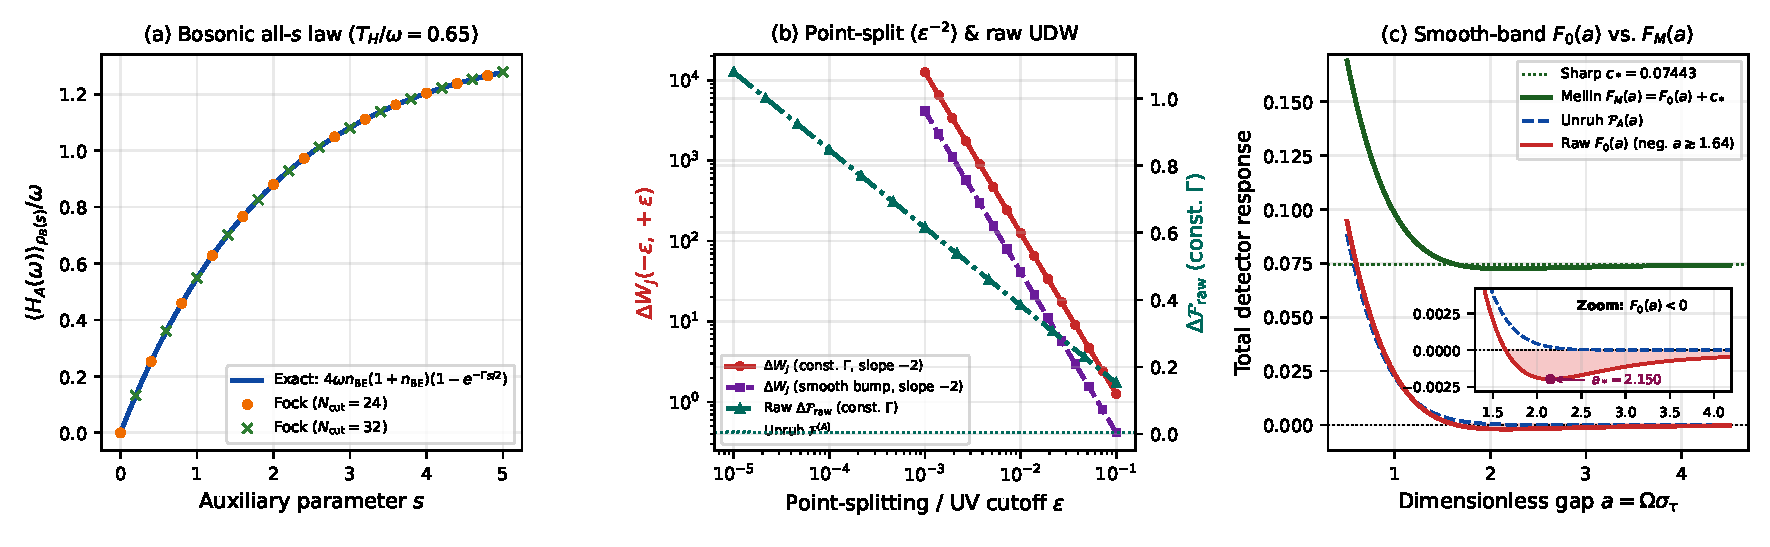
\includegraphics[width=\linewidth]{figures/fig3_horizon_hadamard_udw.pdf}
  \caption{Theorem~\ref{thm:hadamard}, Proposition~\ref{prop:smooth-band-contact}, and numerical audit F4. (a)~Exact bosonic all-$s$ single-mode Hamiltonian law \eqref{eq:unified-all-s} ($\sigma=+1, T_H/\omega=0.65$) verified against truncated Fock substitutions ($N_{\mathrm{cut}}=24, 32$; $8.17\times 10^{-16}$ at $N_{\mathrm{cut}}=32$) and independent \code{solve\_ivp} integration ($N_{\mathrm{cut}}=10$; $4.49\times 10^{-11}$). (b)~Free 2D chiral boson cross-horizon point-split defect $\Delta W_J(-\epsilon,+\epsilon; s=2)$ exhibiting $\epsilon^{-2}$ divergence for both uniform $\Gamma$ and a smooth bump $\Gamma\in C_c^\infty((0,\infty))$ ($\operatorname{supp}\Gamma=[0.5,2.5]$, left axis), alongside the uniform-$\Gamma$ raw-cutoff UDW defect $\Delta\cF_{\mathrm{raw}}\sim\frac{1-e^{-\Gamma s/2}}{2\pi}\ln(\sigma_\tau/\epsilon_{\mathrm{UV}})$ vs.\ smooth Unruh coefficient $\cF^{(A)}=0.003821$ (right axis). (c)~Smooth-band total detector responses vs.\ $a=\Omega\sigma_\tau$: the UV-finite raw response $F_0(a)$ crosses zero near $a=1.643$ for the profile shown (inset: minimum $-0.001979$ at $a_*=2.1501$), whereas the constructive Mellin positive-type extension $F_M(a)=F_0(a)+c_*$ stays strictly positive (lying above $c_*=0.074435$ at smaller gaps such as $F_M(1.5)=0.076472$, and approaching the sharp high-gap asymptote $c_*$ from below for sufficiently large positive gaps as $F_M(a)=c_*-A/\Omega^2+\mathcal{O}(\Omega^{-4})$ with $A>0$).}
  \label{fig:hadamard-udw}
\end{figure}

%==============================================================================
\section{KMS Port-Locking No-Go, Static 4D Greybody Asymptotics, Exact \texorpdfstring{$d_f=1$}{df=1} Erasure, and Separated Benchmark Models}\label{sec:throat}
%==============================================================================

We now audit whether low-energy open gravity and finite-dimensional information theory support universal closure of inward horizon ports ($N_{\mathrm{in}}=0$) without invoking the forbidden loopholes ruled out in Section~\ref{sec:motivation} (holomorphic line-bundle cuts on $S^2\cong\mathbb{CP}^1$ or mid-evaporation single-Hilbert-space local projections).

\paragraph{4D static Schwarzschild perturbation equations across spins $h\in\{0,\frac{1}{2},1,2\}$.}
Reducing 4D general relativity under spherical symmetry $ds_4^2 = g_{\mu\nu}^{(2)}(x)\,dx^\mu dx^\nu + r(x)^2\,d\Omega_2^2$ yields a 2D dilaton theory with $\Phi(x)=r(x)^2/(4G_4)$ (note that near-extremal JT gravity and uncharged 4D Schwarzschild belong to distinct solution families, not a single unified action). On a static 4D Schwarzschild background ($f(r)=1-r_s/r$, tortoise coordinate $r_*=r+r_s\ln(r/r_s-1)$), linearized perturbations of integer spin $h\in\{0,1,2\}$ obey the Regge--Wheeler equation \cite{ReggeWheeler1957,Teukolsky1973}
\begin{equation}\label{eq:regge-wheeler}
  \frac{d^2\psi}{dr_*^2} + \bigl(\omega^2 - V_{h,\ell}(r)\bigr)\psi = 0, \qquad
  V_{h,\ell}(r) = f(r)\!\left(\frac{\ell(\ell+1)}{r^2} + \frac{(1-h^2)r_s}{r^3}\right), \quad \ell \ge h,
\end{equation}
where for $h=2$, \eqref{eq:regge-wheeler} is the odd-parity (axial) gravitational potential, while even-parity (polar) metric perturbations obey the isospectral Zerilli equation \cite{Zerilli1970} sharing identical transmission probabilities $\cT_{2,\ell}(\omega)$. Massless spin-$h=\frac{1}{2}$ Weyl/Dirac perturbations ($\kappa_D=\pm(j+\frac{1}{2})$, $j=\frac{1}{2},\frac{3}{2},\dots$) obey the supersymmetric partner equations
\begin{equation}\label{eq:dirac-4d}
  \frac{d^2 Z_\pm}{dr_*^2} + \bigl(\omega^2 - V_{1/2,\kappa_D}^\pm(r)\bigr) Z_\pm = 0, \qquad
  V_{1/2,\kappa_D}^\pm(r) = \frac{\kappa_D^2 f(r)}{r^2} \pm \frac{|\kappa_D|\sqrt{f(r)}(\frac{3}{2}r_s - r)}{r^3},
\end{equation}
sharing identical greybody transmission probabilities $\cT_{1/2,j}(\omega)$. The single-chirality / single-polarization partial-wave absorption cross section is $\sigma_{\mathrm{abs}}^{(h,j)}(\omega) = \frac{\pi}{\omega^2}(2j+1)\cT_{h,j}(\omega)$ (matching polarization-averaged unpolarized cross sections for $h=1,2$ since both parities are isospectral \cite{Unruh1976Abs,Page1976,Crispino2007}, while summing over two polarizations or chiralities doubles total emitted power).

\begin{theorem}[KMS Port-Locking No-Go, Horizon-Origin Port vs.\ Distant Output Mode, Static 4D Asymptotics, Exact $d_f=1$ Erasure, and Non-Isometric Kernel]\label{thm:throat}
\leavevmode
\begin{enumerate}
  \item[(a)] \emph{(KMS absorption--emission locking on a coupled thermal port and separation of horizon-origin port vs.\ full distant output mode)}
  \begin{enumerate}
    \item[(i)] \emph{(Single coupled thermal KMS port)} In any bosonic open SK model obeying \eqref{eq:fdt}--\eqref{eq:wightman-rates} at finite $T_H = \beta_H^{-1} > 0$, $\omega > 0$, and \emph{nonzero coupling $g \neq 0$}, closing an inward absorption port is algebraically equivalent to extinguishing its Keldysh noise and Hawking emission:
    \begin{equation}\label{eq:kms-locking}
      \rho_{\mathrm{spec}}(\omega) = 0 \;\Longleftrightarrow\; D_K(\omega) = 0 \;\Longleftrightarrow\; \gamma_\downarrow(\omega) = 0 \;\Longleftrightarrow\; \gamma_\uparrow(\omega) = 0,
    \end{equation}
    forcing $\cL_{\mathrm{pair}}=0$ identically (equivalently for effective coupled kernels $\rho_{\mathrm{eff}}:=g^2\rho_{\mathrm{spec}}$, $D_{K,\mathrm{eff}}:=g^2 D_K$). For fermionic linear coupling to anticommuting bath operators, \eqref{eq:fdt} is replaced by the anticommutator spectral density $\rho_{\mathrm{spec}}^{(F)}=G^>+G^<$ and commutator noise kernel $D_K^{(F)}=G^>-G^<=\tanh(\beta_H\omega/2)\rho_{\mathrm{spec}}^{(F)}$, yielding Fermi--Dirac rates $\gamma_\downarrow^{(F)}=g^2(1-n_{\mathrm{FD}})\rho_{\mathrm{spec}}^{(F)}$ and $\gamma_\uparrow^{(F)}=g^2 n_{\mathrm{FD}}\rho_{\mathrm{spec}}^{(F)}$ obeying the same KMS ratio $e^{-\beta_H\omega}$ and four-way vanishing at $\rho_{\mathrm{spec}}^{(F)}=0$.
    \item[(ii)] \emph{(Isolated horizon-origin port $B_{\mathrm{hor}}$ vs.\ full distant canonical output mode $b_{\mathrm{out}}$)} Relating greybody transmission $\cT\in[0,1]$ to \eqref{eq:kms-locking} requires specifying the bath operator. For a \emph{full distant bosonic output mode} $b_{\mathrm{out}} = \sqrt{\cT}\,b_H + \sqrt{1-\cT}\,a_{\mathrm{in}}$ ($b_H$ thermal at occupation $n_H$, $a_{\mathrm{in}}$ independent vacuum) under the canonical chiral-current normalization \eqref{eq:chiral-current-rates} ($\rho_{\mathrm{spec,out}}(\omega)=\omega/2$ independent of $\cT$) and coupling $g\neq 0$ in \eqref{eq:wightman-rates},
    \begin{equation}\label{eq:bout-vs-bhor}
      \begin{aligned}
        D_{K,\mathrm{out}}(\omega) &= \frac{\omega}{2}\bigl(1 + 2\cT n_H\bigr) \ge \frac{\omega}{2} > 0, \\
        \gamma_{\downarrow,\mathrm{out}} &= g^2\frac{\omega}{2}\bigl(1 + \cT n_H\bigr) \ge g^2\frac{\omega}{2} > 0, \qquad
        \gamma_{\uparrow,\mathrm{out}} = g^2\frac{\omega}{2}\cT n_H,
      \end{aligned}
    \end{equation}
    leaving nonzero vacuum noise and spontaneous downward decay $\gamma_{\downarrow,\mathrm{out}}(\cT=0)=g^2\frac{\omega}{2}>0$ even at $\cT=0$ (Test~F5 evaluates the unit-coupling benchmark $g=1$). By contrast, isolating the \emph{horizon-origin thermal port} $B_{\mathrm{hor}} := \sqrt{\cT}\,J_H$ scales both $\rho_{\mathrm{spec,hor}}=\cT\rho_{\mathrm{spec},H}$ and $D_{K,\mathrm{hor}}=\cT D_{K,H}$ linearly with $\cT$, preserves exact KMS detailed balance $\gamma_{\uparrow,\mathrm{hor}}=e^{-\beta_H\omega}\gamma_{\downarrow,\mathrm{hor}}$ for all $\cT\in[0,1]$, and obeys $\cT=0 \iff \rho_{\mathrm{spec,hor}}=0 \iff D_{K,\mathrm{hor}}=0 \iff \gamma_{\downarrow,\mathrm{hor}}=0 \iff \gamma_{\uparrow,\mathrm{hor}}=0$ for any $g\neq 0$ (formalized for arbitrary $g\neq 0$ in \code{distant\_\allowbreak output\_\allowbreak mode\_\allowbreak vacuum\_\allowbreak noise\_\allowbreak vs\_\allowbreak horizon\_\allowbreak port}). Likewise, the normal-ordered emitted Hawking power $P_{\mathrm{Hawking}} = \sum_j \int_0^\infty\frac{d\omega}{2\pi}\,\omega\cT_j(\omega)n_j(\omega)$ vanishes iff $\cT_j(\omega)=0$ for almost every $\omega>0$ across all radiating channels. Note also that $\cL_{\mathrm{pair}}=0$ does not by itself select the singular Boulware vacuum, which is the standard static Killing ground state defined on exterior Schwarzschild \emph{without} a reflective wall \cite{Boulware1975,Candelas1980} (distinct from cavity models imposing a reflective wall).
  \end{enumerate}
  \item[(b)] \emph{(Three distinct conditional algebraic, scattering, and channel results)}
  \begin{enumerate}
    \item[(i)] \emph{(Finite-factorization algebra separation)} On any \emph{assumed} bipartite tensor factorization $\mathrm{Fin}\,d_R \times \mathrm{Fin}\,d_L$ ($d_R, d_L > 0$), every operator $X_R\otimes\1_L$ commutes with every $\1_R\otimes Y_L$, and their intersection is scalar: $(M_{d_R}\otimes\1_L)\cap(\1_R\otimes M_{d_L}) = \bbC\1$. (This is an algebraic lemma for an assumed Cauchy-slice factorization; establishing such a factorization in quantum gravity under diffeomorphism constraints is open, and exterior and future interior spacetime regions are not globally spacelike separated.)
    \item[(ii)] \emph{(Static 4D Schwarzschild fixed-$\omega$ low-frequency absorption asymptotics)} Along the static Schwarzschild family with \emph{fixed} physical frequency $\omega>0$ and $A_{\mathrm{hor}}=4\pi r_s^2\to 0$ ($\tilde{\omega}:=\omega r_s\to 0$, gravitational Sommerfeld factor $S_{\mathrm{Som}}(\tilde{\omega})=\frac{2\pi\tilde{\omega}}{1-e^{-2\pi\tilde{\omega}}}\to 1$) \cite{Unruh1976Abs,Page1976,DasGibbonsMathur1997,GoldbergerRothstein2006,Crispino2007}:
    \begin{equation}\label{eq:all-spin-closure}
      \begin{aligned}
        \sigma_{\mathrm{abs}}^{(0,0)}(\omega) &\sim A_{\mathrm{hor}}, &
        \sigma_{\mathrm{abs}}^{(1/2,1/2)}(\omega) &\sim \tfrac{1}{8} A_{\mathrm{hor}}, \\
        \sigma_{\mathrm{abs}}^{(1,1)}(\omega) &\sim \tfrac{\omega^2}{12\pi} A_{\mathrm{hor}}^2, &
        \sigma_{\mathrm{abs}}^{(2,2)}(\omega) &\sim \tfrac{\omega^4}{720\pi^2} A_{\mathrm{hor}}^3,
      \end{aligned}
    \end{equation}
    so $\sigma_{\mathrm{abs}}^{(h,j)}(\omega)\to 0$ at fixed $\omega$ across all spins $h\in\{0,\frac{1}{2},1,2\}$ and $j\ge|h|$ without spin bypass. Conversely, because $\cT_{h,j}(\omega,r_s)=f_{h,j}(\omega r_s)$ is dimensionless, holding $\omega r_s = a$ fixed (tracking the Hawking peak $T_H=(4\pi r_s)^{-1}$) leaves $\cT_{h,j}$ non-vanishing (e.g.\ $\cT_{0,0}(0.4)=0.9089$) and formal semiclassical power diverges as $P(r_s)\propto r_s^{-2}$, confirming that true evaporation completion lies in the Planckian regime beyond low-energy EFT.
    \item[(iii)] \emph{(Exact complete-erasure identity for a $d_f=1$ intermediate channel)} Whenever a quantum channel factors through a one-dimensional intermediate space $M_1(\bbC)$, every CPTP encoder $\cE: M_{d_C}(\bbC)\to M_1(\bbC)$ and CPTP decoder $\cR: M_1(\bbC)\to M_{d_C}(\bbC)$ forms a replacer channel $\rho\mapsto\tau\Tr\rho$ whose entanglement fidelity on the maximally mixed input $\1/d_C$ obeys the \emph{exact equality}
    \begin{equation}\label{eq:erasure-cap}
      F_e\bigl(\1/d_C,\, \cR\circ\cE\bigr) \;=\; \frac{1}{d_C^2}\sum_{\alpha,\beta}\bigl|\Tr(R_\beta E_\alpha)\bigr|^2 \;=\; \frac{1}{d_C^2}
      \qquad\text{(hence } F_e(\1/d_C, \cR\circ\cE) \le \frac{1}{d_C^2}\text{)},
    \end{equation}
    while for a general input density matrix $\rho$, $F_e(\rho, \cR\circ\cE)=\Tr(\tau\rho^2)$. (Whether dynamical gravitational evaporation actually reaches $d_f=1$ is an external physical assumption, not proved by this channel identity.)
  \end{enumerate}
  \item[(c)] \emph{(Non-isometric rank-nullity and non-trace-preserving obstruction \cite{Akers2022})} For any linear encoding $V:\bbC^{d_{\mathrm{eff}}}\to\bbC^{d_{\mathrm{fund}}}$ with $d_{\mathrm{fund}} < d_{\mathrm{eff}}$, $\ker V$ contains a nonzero bulk null state ($\exists\psi\neq 0,\,V\psi=0$) and $V^\dagger V \neq \1_{d_{\mathrm{eff}}}$. Consequently, the naive conjugation map $\rho\mapsto V\rho V^\dagger$ cannot define a trace-preserving CPTP channel on $\mathcal{B}(\bbC^{d_{\mathrm{eff}}})$, since any unit null vector $\psi\in\ker V$ obeys $\Tr(V|\psi\rangle\langle\psi|V^\dagger)=0\neq 1$.
\end{enumerate}
\end{theorem}

\begin{proof}
Following Table~\ref{tab:lean}'s granularity, the algebraic bosonic port-locking equivalences \eqref{eq:kms-locking}, distant-mode vs.\ horizon-port separation \eqref{eq:bout-vs-bhor} for arbitrary $g\neq 0$, finite-factorization algebra separation, rank-nullity non-TP witness, and $d_f=1$ replacer erasure \eqref{eq:erasure-cap} are formalized in \code{OSTQD\_\allowbreak SK/\allowbreak Theorem4\_\allowbreak Non\allowbreak Isometric\allowbreak Throat.\allowbreak lean} (\code{kms\_\allowbreak in\allowbreak ward\_\allowbreak port\_\allowbreak lock\allowbreak ing\_\allowbreak nogo}, \code{dis\allowbreak tant\_\allowbreak out\allowbreak put\_\allowbreak mode\_\allowbreak vac\allowbreak uum\_\allowbreak noise\_\allowbreak vs\_\allowbreak hori\allowbreak zon\_\allowbreak port}, \code{exter\allowbreak ior\_\allowbreak inter\allowbreak ior\_\allowbreak alge\allowbreak bra\_\allowbreak sepa\allowbreak ration}, \code{non\allowbreak iso\allowbreak metric\_\allowbreak ker\allowbreak nel\_\allowbreak non\allowbreak trivial}, \code{throat\_\allowbreak clo\allowbreak sure\_\allowbreak com\allowbreak plete\_\allowbreak era\allowbreak sure\_\allowbreak eq}, and \code{throat\_\allowbreak clo\allowbreak sure\_\allowbreak com\allowbreak plete\_\allowbreak era\allowbreak sure\_\allowbreak bound}). Fermionic anticommutator FDT conventions, the multi-port total Hawking power integral, and the 4D Schwarzschild scattering ODEs lie outside Lean: part~(b.ii) is verified numerically on five representative channels in Section~\ref{sec:numerics}, while higher partial waves follow established analytic scattering asymptotics \cite{Unruh1976Abs,Page1976,DasGibbonsMathur1997,GoldbergerRothstein2006,Crispino2007}. Note that \eqref{eq:erasure-cap} is a direct replacer-channel corollary of the bottleneck bound \cite{Soga2026OSTQD,FarberGour2026}: any trace-preserving encoder into $M_1(\bbC)$ acts as $\cE(X)=\Tr(X)$ and any CPTP decoder as $\cR(z)=z\tau$ ($\Tr\tau=1$), so $F_e(\1/d_C,\cR\circ\cE)$ $=\langle\Phi_{d_C}|(\1_R/d_C\otimes\tau)|\Phi_{d_C}\rangle = 1/d_C^2$.
\end{proof}

Bringing together Theorems~\ref{thm:covariant-kms}, \ref{thm:hadamard}, and~\ref{thm:throat} with Proposition~\ref{prop:smooth-band-contact} clarifies the exact condition-indexed scope of a heuristic often raised for distant observer $B$---namely, that ``for $B$, a black hole is the event horizon itself, with the interior and singularity undefined (or lying solely in the future), so that the infall path is closed''---while keeping distinct causal, thermal, distributional, and dynamical hypotheses strictly separated:

\begin{proposition}[Condition-Indexed Obstruction Summary on Closed-Infall Models and Open Exterior-Boundary Proposal]\label{prop:closed-infall-nogo}
\leavevmode
\begin{enumerate}
  \item[(I)] \emph{(Causal-past restriction vs.\ future-access quantification)} Because $\mathcal{H}^+ = \partial J^-(\mathcal{I}^+)$, the black-hole interior $I := M\setminus J^-(\mathcal{I}^+)$ satisfies $I\cap J^-(p_B)=\emptyset$ for every exterior point $p_B\in J^-(\mathcal{I}^+)$, and the future interior singularity of the assumed collapse geometry lies outside $J^-(p_B)$. Hence interior degrees of freedom do not act as direct causal-past sources inside $B$'s exterior causal algebra $\cA(W_B)$. (In a \emph{static} Schwarzschild geometry, infalling trajectories reach $r=r_s$ only as static Killing time $t\to+\infty$; a general evaporating spacetime admits no global static Killing time.) Conversely, future causal access $J^+(p_B)\cap I\neq\emptyset$ holds specifically for exterior points in $J^-(I)$, not unconditionally for arbitrarily distant points emitted too close to complete evaporation in a finite-lifetime black-hole geometry.
  \item[(II)] \emph{(Four condition-indexed low-energy obstructions)} Because the models below rely on distinct hypotheses, they do not form a single universal no-go theorem over all conceivable horizon-only theories; rather, each isolates a specific obstruction specifying which assumption must be altered to evade it:
  \begin{enumerate}
    \item \emph{Future causal access on $J^-(I)$:} By definition of $J^-(I)$, every exterior point $p_B\in J^-(I)$ admits a future-directed causal curve entering $I$ across $\mathcal{H}^+$ ($\mathcal{H}^+$ is one-way open inward, closed outward; asserting a maximizing timelike geodesic requires stronger assumptions such as $p_B\in I^-(\mathrm{Int}\,I)$ within a globally hyperbolic regular region).
    \item \emph{Per-port dynamical KMS absorption--emission locking (Theorem~\ref{thm:throat}(a)):} On the isolated horizon-origin thermal port $B_{\mathrm{hor}}=\sqrt{\cT_{h,j}(\omega)}\,J_H$ at $T_H>0$ (distinct from the full distant output mode $b_{\mathrm{out}}$, which retains vacuum noise $\omega/2$ even at $\cT=0$), setting $\cT_{h,j}(\omega)=0$ extinguishes that port's spectral density, Keldysh noise, and upward/downward rates; extinguishing total normal-ordered Hawking power $P_{\mathrm{Hawking}}=\sum_j\int_0^\infty\frac{d\omega}{2\pi}\,\omega\cT_j(\omega)n_j(\omega)$ requires $\cT_j(\omega)=0$ for almost every $\omega>0$ across \emph{all} bosonic and fermionic radiating channels (recalling from \S\ref{sec:jt-sk} that the full Unruh state is non-KMS, and that Boulware horizon stress divergence \cite{Boulware1975,Candelas1980} characterizes the wall-free static Killing ground state rather than a reflective cavity alone).
    \item \emph{Free-chiral-boson off-horizon dephasing obstruction and sharp point-contact floor (Theorem~\ref{thm:hadamard}(b), Proposition~\ref{prop:smooth-band-contact}):} For the specified free $c=1$ chiral current under modewise exterior $N_{R,\omega}$-dephasing with $s>0$ and $\Gamma\ge 0$ nonzero on a positive-measure frequency set, \emph{every} extension agreeing with the off-horizon kernel---including axis-supported modifications---breaks Hadamard regularity at $\mathcal{O}(\epsilon^{-2})$ by \eqref{eq:hadamard-defect}. Under Proposition~\ref{prop:smooth-band-contact}'s additional smooth compact-band hypothesis $0\not\equiv\Gamma\in C_c^\infty((0,\infty))$ ($\Gamma\ge 0$, $s>0$, excluding constant $\Gamma_0>0$ where \eqref{eq:mellin-cstar} diverges as $\omega^{-2}$ at $\omega\to 0$ and \eqref{eq:udw-div} diverges logarithmically), restricting to positive-type finite-order point-contact extensions of $T_0$ at $(0,0)$ forces the finite sharp threshold $c_{00}\ge c_* > 0$ (both necessary and sufficient at zero order via $T_M$) and a non-decaying high-gap excitation floor. (Arbitrary nonlocal membranes, interacting/non-Gaussian horizon models, nonlinear detectors \cite{Zambianco2026}, Louko's distinct distributional prescription \cite{Louko2014}, and non-point-contact positive extensions lie outside this classification.)
    \item \emph{Free-subsystem Markovian regression criterion (Theorem~\ref{thm:covariant-kms}(f)):} Any nontrivial KMS dissipator acting on $\cA_B$ ($L\notin\cA_B'$) departs from \emph{free-subsystem} two-time autocorrelations $C_{\mathrm{free}}(\tau)$ on non-commuting observables, though Markovian quantum regression matches interacting total-system unitary correlations $C_{\mathrm{total}}(\tau)$ at discrete repeated-interaction steps or in the unitary Markov-dilation limit \cite{Frigerio1985,AttalJoye2007}.
  \end{enumerate}
  \item[(III)] \emph{(Conditional exterior-boundary proposal and unresolved scope)} Together with Theorem~\ref{thm:throat}(b.ii) (fixed-$\omega$ static absorption $\sigma_{\mathrm{abs}}\to 0$ as $A_{\mathrm{hor}}\to 0$, contrasted with non-vanishing Hawking-peak $\cT_{0,0}(\omega r_s=0.4)=0.9089$) and Remark~\ref{rem:three-endpoints} (three ununified low-energy endpoints), these condition-indexed audits motivate modeling $B$'s low-energy exterior description at $A_{\mathrm{hor}}>0, T_H>0$ as an \emph{asymmetrically open dissipative horizon boundary} (SK influence functional with active inward absorption channels) rather than a severed horizon-only wall, without establishing a universal closed-infall no-go theorem, universal closure exclusively at $A_{\mathrm{hor}}\to 0$, or a general necessity of non-Markovian bath memory. Because any Layer~1 SK reduction remains a non-selective trace-out, explaining single-shot Layer~2 factual divergence between $A$ and $B$ remains open (Remark~\ref{rem:layer2-gauge}, Proposition~\ref{prop:layer2-singleshot}).
\end{enumerate}
\end{proposition}

\begin{remark}[Distinction among three low-energy endpoints and three separated F6 benchmark models]\label{rem:three-endpoints}
Three limitations prevent collapsing Theorem~\ref{thm:throat} and Test~F6 into a single unified dynamical evaporation theorem:
\begin{enumerate}
  \item \emph{Three distinct endpoints:} In the 2D JT saddle of Theorem~\ref{thm:jt-sk}(b), $S_{\mathrm{BH}}(u)\to S_0 > 0$ as $u\to\infty$; for our benchmark $S_0 = 20$, $\exp(S_0) \approx 4.85\times 10^8 \neq 1$, distinct from both uncharged 4D Schwarzschild ($A_{\mathrm{hor}}\to 0$, where $C_V<0$ and fixed-$\omega r_s$ Hawking-peak transmission stays $\mathcal{O}(1)$) and a discrete qubit model reaching $d_{\mathrm{BH}}=1$.
  \item \emph{Three separate conditional models in Test~F6:} Test~F6 independently audits: (Model~1)~the simplified JT entropy crossing $S_{\mathrm{Page}}(u)=\min(S_{\mathrm{Hawking}}(u), S_{\mathrm{BH}}(u))$ at $S_{\mathrm{BH}}(u_{\mathrm{Page}})=\frac{2}{3}S_{\mathrm{BH}}(0)$---which occurs at finite $u_{\mathrm{Page}}$ iff $S_0 < 8\pi^2 C T_0$ (satisfied here since $20 < 947.48$, an algebraic benchmark distinct from full QES extremization \cite{AEMM2019} approaching $S_0=20$ nats at late times); (Model~2)~a static $64\to 32$ Haar post-selected map $V=\sqrt{2}PU$, obeying exact operator-norm non-isometry $\|V^\dagger V - \1\|_{\mathrm{op}}=1.0$, non-trace-preserving null-state collapse $\Tr(V|\psi_{\mathrm{null}}\rangle\langle\psi_{\mathrm{null}}|V^\dagger)=2.57\times 10^{-31}\neq 1$, and basis off-diagonal RMS $\mathcal{O}(d_{\mathrm{fund}}^{-1/2})$ (distinct from the uniform probabilistic concentration over bounded-complexity state sets proved in \cite{Akers2022}); and (Model~3)~separate isometric $N=8$-qubit Haar-scrambled diary models: for $d_C=2$, $F_{\mathrm{rad}}:0.25\to 1.0$, $F_{\mathrm{rem}}:1.0\to 0.25$ with cap sequence $(1,\dots,1,1/4)$ (so the nontrivial dimensional bottleneck occurs only at the $k=8$ erasure endpoint, where final $S_{\mathrm{rad}}=1$~bit reflects maximal entanglement with reference $R$), complemented by a $d_C=4$ (2-qubit diary) audit exercising the nontrivial intermediate bottleneck $d_{\mathrm{BH}}=2<d_C=4$ at $k=7$ ($F_{\mathrm{rem}}(7)=0.0660\le 1/4$) before exact erasure $F_{\mathrm{rem}}(8)=1/16$ at $k=8$. Connecting these three models requires specifying a physical CPTP radiation channel and dynamical state-space map $V_u$, which remains open.
\end{enumerate}
\end{remark}

Figure~\ref{fig:throat-noniso} illustrates both the static 4D Schwarzschild fixed-$\omega$ greybody audit (Test~F5) and the separate 8-qubit diary model (Test~F6, Model~3).

\begin{figure}[!tb]
  \centering
  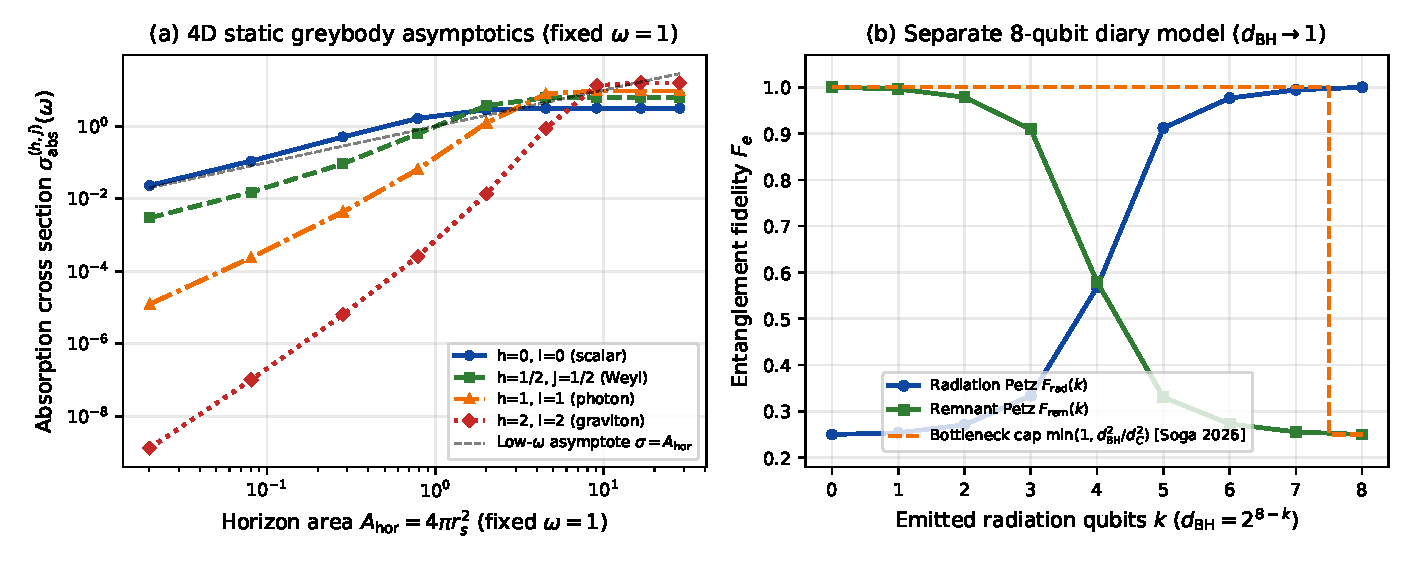
\includegraphics[width=\linewidth]{figures/fig4_greybody_throat_and_nonisometric.pdf}
  \caption{Theorem~\ref{thm:throat} and numerical audits F5--F6. (a)~Direct \code{wrightomega}-inverted numerical scattering integration of static 4D Schwarzschild Regge--Wheeler \eqref{eq:regge-wheeler} and Dirac \eqref{eq:dirac-4d} equations at fixed $\omega=1$ as $A_{\mathrm{hor}}=4\pi r_s^2\to 0$: all four simulated lowest partial waves ($h\in\{0,\frac{1}{2},1,2\}$) track their low-$\omega$ asymptotics \eqref{eq:all-spin-closure} to zero (note that at finite $\tilde{\omega}$, the scalar curve sits slightly above the asymptotic dashed line $\sigma=A_{\mathrm{hor}}$ due to the gravitational Sommerfeld enhancement $S_{\mathrm{Som}}(\tilde{\omega})\approx 1+\pi\tilde{\omega}$). (b)~Separate isometric $N=8$-qubit scrambled diary model ($d_C=2, d_{\mathrm{BH}}=2^{8-k}$): radiation Petz fidelity $F_{\mathrm{rad}}(k)$ rises from $0.25$ to $1.00$ while remnant fidelity $F_{\mathrm{rem}}(k)$ drops from $1.00$ to $0.25$, obeying the bottleneck cap $\min(1, d_{\mathrm{BH}}^2/d_C^2)$ \cite{Soga2026OSTQD,FarberGour2026} and attaining the exact $d_f=1$ erasure value $1/d_C^2=0.25$ at $k=8$.}
  \label{fig:throat-noniso}
\end{figure}

%==============================================================================
\section{Categorized Numerical Verification Audit (Suites F1--F6)}\label{sec:numerics}
%==============================================================================

Our deterministic script (\code{scripts/\allowbreak verify\_\allowbreak paper2\_\allowbreak sk\_\allowbreak jt.\allowbreak py}, seed \code{20261127}, Python~3.14.7, NumPy~2.4.2, SciPy~1.17.1, Matplotlib~3.10.8; 309 recorded scientific numeric fields across F1--F6 in \code{docs/\allowbreak numer\allowbreak ical\_\allowbreak veri\allowbreak fication.\allowbreak json}, excluding metadata---comprising input parameters, arrays, algebraic checks, negative controls, ODE/scattering integrations, and zero time-discretization bias Monte Carlo estimates, not 309 independent physical experiments) executes six categorized verification suites:
\begin{itemize}
  \item \textbf{F1 (Microscopic kernel normalization, Layer-2 unraveling gauge, no-signaling vs.\ model-compatibility, chiral Fourier check, QND bath response, SK non-sufficiency, two-bath non-KMS, and Redfield CP failure):}
  \emph{Algebraic / microscopic checks:} SK axioms \eqref{eq:sk1}--\eqref{eq:sk3} ($0.0$ residual); 80-level harmonic-bath characteristic function matches the consistent $N(t=0)=D_K(t=0)/2$ normalization \eqref{eq:fv-quad} to $1.11\times 10^{-16}$ (vs.\ $0.0760$ mismatch for doubled noise); regulated vacuum chiral-current Fourier quadrature matches $(\Omega/2)e^{-\epsilon\Omega}$ to $1.44\times 10^{-15}$ (with thermal Bose factor entering algebraically via KMS); Davies CPTP across $T_H/\omega\in[0.25,5.0]$, $s\in[0.05,3.0]$ ($\min\lambda(J)=+1.88\times 10^{-6}$, TP error $4.97\times 10^{-16}$); Layer-2 orthogonal Kraus gauge $(u,v)=(0.6,0.8)$ leaves the Layer-1 CPTP map invariant ($0.0$) while shifting single-shot $p_0(|0\rangle\langle 0|):1.0\to 0.36$ and conditional coherence on $|+\rangle\langle +|:0.0\to 0.48$; local Pauli-$X$ unitary $X_R\otimes\1_L$ preserves remote marginal $\rho_L$ identically ($0.0$) while mismatching target dephasing by $0.8485$.
  \emph{Negative controls:} $3\times 3$ Hadamard multiplier satisfies pointwise SK1--SK3 yet has $\min\lambda(M/3)=-0.07459 < 0$ (Remark~\ref{rem:sk-nonsuff}); QND bath-response controls confirm $D_R(t)=-0.78950\neq 0$ (oscillator bath) and $\mathrm{Re}\,D_R(0)=-2.5465\neq 0$ (Ohmic continuum); two-bath Unruh ratio $0.22540 \neq e^{-1}=0.36788$; two-level $\sigma_x$ Redfield yields strictly negative Choi eigenvalues at every finite $T_H$ ($-2.00\times 10^{-3}$ at $T_H/\omega=0.25$).
  \item \textbf{F2 (Fixed-$T_H$ covariant $(t,s)$ identities, non-commuting GNS $\chi^2$, free-subsystem QRT criterion, 3-level diffusion, Duhamel holonomy bound, and uniform contraction Gibbs tracking):}
  \emph{Algebraic / semigroup checks:} On $d=6$ ($\omega=1.2, T_H=0.65$), KMS stationarity ($1.40\times 10^{-17}$), energy flux and carr\'e du champ ($2.42\times 10^{-15}$, $2.07\times 10^{-14}$), $(t,s)$ commutation ($1.01\times 10^{-15}$), GNS Dirichlet identity ($3.58\times 10^{-15}$), diagonal cooling ($D: 2.995\to 0.116$, $\chi^2_{\beta_H}: 398.7\to 0.356$, purity $0.167\to 0.505$), and full non-commuting symmetric $B_s$ audit ($D: 1.623\to 0.0718$, $\chi^2_{\beta_H}: 101.96\to 0.252$, intertwining $3.55\times 10^{-13}$, derivative $5.68\times 10^{-14}$); 2-level asymmetric $A_L$ failure ($0.5625$) vs.\ symmetric $B$ exact agreement ($2.29\times 10^{-16}$); free-subsystem QRT Dirichlet witness ($0.0$ for commuting $\1\otimes\sigma_z$ vs.\ $1.25$ for non-commuting $\sigma_x\otimes\1$, residual $0.0$).
  \emph{Negative controls and Proposition~\ref{prop:nonstationary} tracking bounds:} 3-level counterexample ($\|\cL^\dagger(H_3)\|=0$, $\mathrm{Var}(H_3)_{s=1}=0.864665$); non-stationary $T(t)=e^{-0.3t}$ (Duhamel holonomy trace norm $0.01648 \le \Delta s\|\Delta\cL\|_{1\to 1}=0.02025$ $\le \Delta s\Delta t\sup\|\partial_\tau\cL\|_{1\to 1}=0.02210$, moving-Gibbs $D(\rho_{0.5}\|\sigma_{0.5})=0.001724>0$); slow-relaxation tracking counterexample ($\mu=10^{-4},\eta=10^{-8}$, $\max|\dot{T}|/T^2=2\times 10^{-4}$, exact peak $\sup\|\dot{\sigma}\|_1=4.477432\times 10^{-5}$ at $z=1.543405$, yet trace distance $\frac{1}{2}\|\rho-\sigma\|_1 = 0.14973$ and trace norm $\|\rho-\sigma\|_1 = 0.29946 \le 0.31034$); fast-relaxation positive control ($\eta=0.1$, observed diagonal $\max\|\rho_t-\sigma_t\|_1 = 3.1984\times 10^{-4}$ obeying both the diagonal-subspace bound $3.4100\times 10^{-4}$ at $\lambda_{\mathrm{diag}}=0.13130$ and the full traceless-Hermitian uniform bound $6.8200\times 10^{-4}$ at $\lambda_{\mathrm{full}}=0.06565$, off-diagonal $\sigma_x$ rate check $0.0$); non-secular commutator breaking ($22.065$, $0.875$).
  \item \textbf{F3 (2D JT + CFT Ward ODE, exact-step Gaussian \& frozen-coefficient compound-Poisson MC, state-dependent $K_3$, three-tier equilibrium closure comparison, finite-$q$ detailed balance, generator integral, and $Z_C(\beta)$):}
  \emph{ODE/quadrature, equilibrium hierarchy \& detailed balance:} At $C=12, c=24, S_0=20, T_0=1$ (Markov ratio $\gamma_E/T_0=0.0265$), \code{DOP853} Ward ODE matches $E_0 e^{-\gamma_E u}$ to $7.60\times 10^{-12}$; flux balance $1.78\times 10^{-15}$; chiral noise integral to $8.88\times 10^{-16}$; leading equilibrium FDT residual $0.0$ (1-loop disk correction $0.317\%$ at $CT_0=12$). State-dependent leading $K_3^{\mathrm{state,lead}}(30)=+28.29$ (vs.\ frozen $-158.80$) matches independent ODE integration to $3.52\times 10^{-15}$. Three-tier fixed-BD-coefficient equilibrium closure comparison verifies Tier~1 ($K_3^{\mathrm{lin}}=0$, $K_4^{\mathrm{lin}}/\kappa_4^{\mathrm{can}}=0.5$), Tier~2 ($K_3^{\mathrm{Gauss}}/\kappa_3^{\mathrm{can}}=1.0$, $K_4^{\mathrm{Gauss}}/\kappa_4^{\mathrm{can}}=1.5$), Tier~3 ($K_4^{\mathrm{KM}}/\kappa_4^{\mathrm{can}}=1.0$), and Hamilton--Jacobi zero-locus residual $0.0$ across $E/E_0\in[0.2,3.0]$. Finite-$q$ detailed-balance audit confirms naive BD log-ratio errors $1.49\times 10^{-5}$ to $0.5956$ across $q\in[0.2,15]$ vs.\ exact $0.0$ residual for \eqref{eq:ediff-jump-kernel} (curvature agreement $1.06\times 10^{-4}$ at $q=0.05$); independent generator-integral stationarity check for the test function $f(E)=e^{-0.1E}$ at $\alpha=1, C=0.5, \beta_0=1.2$ cancels incoming $-0.03019737093214$ against outgoing $+0.03019737093214$ to $1.89\times 10^{-15}$ (vs.\ $+0.00632818$ for naive $q>E$-rejected emission), direct quadrature matches $Z_C(1.2)$ in \eqref{eq:ediff-partition} to $6.90\times 10^{-16}$, and $C=12, \beta_0=1$ stationary cumulants $\kappa_1,\dots,\kappa_4$ match \eqref{eq:ediff-cumulants} to $8.42\times 10^{-13}$.
  \emph{Zero time-discretization bias Monte Carlo (sampling error of the simulated closure):} Gaussian exact-step MC ($2\times 10^4$ paths, \code{ddof=1}) matches equilibrium variance to $2.10\%$ and $V(u)$ to $0.31\%$ at $u=187.57$ ($CT_H=0.997$) and $0.43\%$ at $0.65 u_{\mathrm{break}}$ ($P(E<0)=1.02\%$ at $CT_H=1$). Continuous-time non-homogeneous compound-Poisson MC ($10^5$ paths) for the frozen-coefficient additive closure matches $K_2, K_3$ to $0.46\%, 2.18\%$ at $u_{CT=1}$ (MC $\gamma_1=-0.1938$ vs.\ $-0.1910$) and $K_2, K_3, K_4$ to $0.50\%, 0.72\%, 0.15\%$ at $u_{\mathrm{break}}$ (MC $\gamma_1=-0.7549, \gamma_2=+1.0201$).
  \item \textbf{F4 (Bosonic all-$s$ ODE, smooth-band Mellin extension $T_M$ \& sharp $c_*$, Dawson cross-check, band-split $Q_\ell$ decay, single-mode four-point distinction, number-projective single-shot floor, and free-subsystem QRT contrast):}
  \emph{Analytic substitution \& ODE:} Truncated Fock matches to $5.78\times 10^{-14}$ ($N_{\mathrm{cut}}=24$), $8.17\times 10^{-16}$ ($N_{\mathrm{cut}}=32$), $\mathcal{O}(Nq^N)$ formula to $4.44\times 10^{-16}$, and independent \code{solve\_ivp} ($N_{\mathrm{cut}}=10$) to $4.49\times 10^{-11}$.
  \emph{Quadrature, Mellin $T_M$ \& controls:} Fixed-$s$ exterior CPL $2.51\times 10^{-16}$; cross-horizon integral $2.86\times 10^{-16}$; smooth-bump point-split slope $-2.0000000000000004$ vs.\ UV-finite raw-cutoff defect ($-0.001783$ at $\Omega=1.5$, cutoff change $3.36\times 10^{-9}$); uniform-$\Gamma$ raw slope matches $(1-e^{-1})/(2\pi)$ to $3.14\times 10^{-9}$; smooth-bump $F_0(a)$ turns negative at $a=2$ ($-0.001877$) and $a=3$ ($-0.001121$), matches $-A/\Omega^2$ ($A=0.00672062$) to $0.97\%$ at $\Omega=16$, obeys $\sigma_\tau$-invariance ($0.0$), matches independent Dawson quadrature to $2.95\times 10^{-17}$, and attains Gaussian witness $-F_0(2.1501)\approx 0.00197949$. Sharp Mellin contact constant $c_*=0.074434671717$ matches direct wide-panel angular quadrature to $9.50\times 10^{-10}$ and $\operatorname{sech}^2$ IBP to $1.26\times 10^{-15}$; direct Mellin quadrature of $F_M(a)$ matches $F_0(a)+c_*$ to $4.70\times 10^{-15}$ ($F_M(2.1501)=+0.07245518 < F_M(16)=0.07440817 < F_M(48)=0.07443175 < c_*$); band-split oscillatory quadrature over $0\le k\le 240$ (vs.\ $k_{\max}=150$ diff $2.66\times 10^{-15}$) yields $\langle T_M,Q_\ell\otimes\overline{Q_\ell}\rangle = 0.42520870, 0.11243000, 0.00804573, 0.000787335$ ($\ell=1,10,10^2,10^3$); single-mode four-point Sperling--Vogel vs.\ quasifree $\langle N_R N_L\rangle$ equals $0.42293033$ vs.\ $0.12187693$; single-shot floor $2\omega n_{\mathrm{BE}}=0.54683$, $\|[P_A,P_B]\|_F=0.58071$; free-subsystem QRT ratio $0.60653=e^{-1/2}$.
  \item \textbf{F5 (Near-horizon-stabilized 4D static Schwarzschild scattering, separated convergence audits, fixed-$\omega r_s$ control, and $b_{\mathrm{out}}$ vs.\ $B_{\mathrm{hor}}$ port audit):}
  Integrates \eqref{eq:regge-wheeler}--\eqref{eq:dirac-4d} across five channels ($h=0,\ell=0,1$; $h=\frac{1}{2},j=\frac{1}{2}$; $h=1,\ell=1$; $h=2,\ell=2$) via near-horizon-stabilized \code{wrightomega} inversion ($\delta=\mathrm{wrightomega}(x-1)$, $f=\delta/(1+\delta)$) and \code{DOP853} ($r_{\mathrm{tol}}=10^{-12}$): max relative Wronskian residual (normalized by $|A_{\mathrm{in}}|^2$) $9.11\times 10^{-12}$ (max absolute $1.63\times 10^{-5}$ overall due to finite-precision cancellation in $|A_{\mathrm{in}}|^2-|A_{\mathrm{out}}|^2$ at ultra-small $\cT$, $3.15\times 10^{-9}$ for $\cT>10^{-6}$); inner-boundary shifts ($x_{\min}=-45\to -80$) $\le 8.79\times 10^{-9}$; outer-matching shifts ($c_{\mathrm{out}}=120\to 240$) $\le 3.00\times 10^{-7}$ (Dirac $(-80,480)$ shift $9.34\times 10^{-9}$; naive $f=1-1/y$ rounding shift $-6.76\times 10^{-7}$); Dirac SUSY $2.13\times 10^{-7}$; ultra-low benchmarks (scalar $\sigma/A=1.01636$, Weyl $0.12708$, photon $\cT/\tilde{\omega}^4=0.45931$, graviton $\cT/\tilde{\omega}^6=0.019019$); fixed-$\omega r_s=0.4$ control $\cT_{0,0}=0.90894$; KMS linear shutdown to $0.0$; distant-mode vs.\ horizon-port control at $\omega=0.4$ and unit coupling $g=1$ confirms $D_{K,\mathrm{out}}(\cT=0)=\gamma_{\downarrow,\mathrm{out}}(\cT=0)=0.2 > 0$ vs.\ $D_{K,\mathrm{hor}}(\cT=0)=0.0$ (horizon-port KMS ratio error $1.13\times 10^{-17}$).
  \item \textbf{F6 (Three separated conditional benchmark models):}
  Model~1 (simplified JT crossing): $u_{\mathrm{Page}}=32.18$ (residual $1.14\times 10^{-13}$), extremal $e^{S_0}=4.85\times 10^8$. Model~2 (static $64\to 32$ Haar map $V$): rank $32$, nullity $32$, null-state trace $2.57\times 10^{-31}\neq 1$, exact $\|V^\dagger V-\1\|_{\mathrm{op}}=1.000000$, basis off-diagonal RMS $[0.1763, 0.1254, 0.0884, 0.0625]$ across $d_{\mathrm{fund}}\in\{16,32,64,128\}$. Model~3 (separate $N=8$ isometric diary models): for $d_C=2$, $F_{\mathrm{rad}}:0.25\to 1.0$, $F_{\mathrm{rem}}:1.0\to 0.25$ (cap sequence $(1,\dots,1,1/4)$), $\max(F_{\mathrm{rad}}+F_{\mathrm{rem}})=1.2500<1.5$, final $S_{\mathrm{rad}}=1.000$~bit; for $d_C=4$, nontrivial intermediate bottleneck $F_{\mathrm{rem}}(7)=0.0660\le 0.25$ at $d_{\mathrm{BH}}=2$ and exact erasure $F_{\mathrm{rem}}(8)=0.0625=1/16$ at $d_{\mathrm{BH}}=1$.
\end{itemize}

Table~\ref{tab:numerics} summarizes all six verification suites by audit category.

\begin{table}[!tb]
\centering\scriptsize\setlength{\tabcolsep}{3.8pt}
\caption{Summary of categorized numerical verification suites F1--F6 (\code{scripts/verify\_\allowbreak paper2\_\allowbreak sk\_\allowbreak jt.py}, seed \code{20261127}, 309 recorded scientific numeric fields across F1--F6).}
\label{tab:numerics}
\begin{tabular}{@{}>{\raggedright\arraybackslash}p{0.24\linewidth}>{\raggedright\arraybackslash}p{0.13\linewidth}>{\raggedright\arraybackslash}p{0.31\linewidth}>{\raggedleft\arraybackslash}p{0.25\linewidth}@{}}
\toprule
Suite & Audit type & Criterion / contrast & Observed value / error \\
\midrule
F1: Bath, vac.\ Fourier, L2 & Micro.\ check & $N(t=0)=D_K/2$; vac.\ $\frac{\Omega}{2}e^{-\epsilon\Omega}$; NS / ch. & $1.11\times 10^{-16}$; $1.44\times 10^{-15}$; $0.0$ / $0.849$ \\
F1: SK, bath $D_R$, 2-bath, Redf. & Neg.\ controls & $\lambda_{\min}(M/3)$; $D_R\neq 0$; $r_{\mathrm{2b}}$; Choi & $-0.0746$; $-0.7895$; $0.2254$; $-2.00\times 10^{-3}$ \\
F2: Fixed-$T_H$, sym.\ $B_s$, QRT & Algebraic & Intertwining; $d\chi^2/ds$; QRT decay & $3.55\times 10^{-13}$; $5.68\times 10^{-14}$; $0.0$ vs.\ $1.25$ \\
F2: Duhamel, tracking, 3-lvl & Neg.\ + pos. & Holonomy; slow ($\frac{1}{2}\|\cdot\|_1$) / fast (diag / full) & $0.0165$; $0.299$ ($0.150$) / $3.20\times 10^{-4}\le 3.41,6.82\times 10^{-4}$ \\
F3: JT Ward, 3-tier, state $K_3$, DB & ODE / alg. & Ward; $K_3$; gen.\ int.\ exact / naive; $\kappa_n$ & $7.60\times 10^{-12}$; $-158.8$ / $+28.3$; $1.9\times 10^{-15}$ / $0.0063$; $8.4\times 10^{-13}$ \\
F3: Gaussian \& frozen CP MC & MC sampling & $Q_{\mathrm{exact}}$ ($CT\simeq 1$); CP $K_2/K_3/K_4$ ($u_{\mathrm{brk}}$) & $0.31\%$; $0.50\%$ / $0.72\%$ / $0.15\%$ \\
F4: Boson ODE, Mellin $T_M$, $c_*$ & Quad.\ + ODE & $N=32$; $c_*$ / $F_M(a_*)$; Mellin / Dawson & $8.2\times 10^{-16}$; $0.07443$ / $0.07246$; $4.7\times 10^{-15}$ / $3\times 10^{-17}$ \\
F4: Point-split, $F_0$, $Q_\ell$, 4-pt & Neg.\ controls & $F_0(a_*)$; $Q_\ell$ ($1\to 10^3$); 4-pt SV / QF & $-0.001979$; $0.4252\to 7.87\times 10^{-4}$; $0.4229$ vs.\ $0.1219$ \\
F5: Stabilized 4D Schw.\ (5 ch.) & ODE + conv. & Rel.\ Wron.\ ($/|A_{\mathrm{in}}|^2$); in/out; $b_{\mathrm{out}}$ vs.\ $B_{\mathrm{hor}}$ & $9.11\times 10^{-12}$; $\le 3.0\times 10^{-7}$; $0.2$ vs.\ $0.0$ \\
F5: Low-$\tilde{\omega}$ vs.\ fixed $\omega r_s$ & Bench.\ + ctrl & DGM $1.016$, Unruh $0.127$; $\cT_{0,0}(0.4)$ & Fixed $\omega,\,r_s\to 0$; $\cT_{0,0}(0.4)=0.9089$ \\
F6: 3 separate benchmarks & Algebraic & JT $e^{S_0}$; null $\Tr$; $d_C=2,4$ Petz & $4.85\times 10^8$; $2.6\times 10^{-31}$; $0.25$ / $0.066\to 0.0625$ \\
\bottomrule
\end{tabular}
\end{table}

%==============================================================================
\section{Lean~4.36.0 Formal Verification and Trust Boundary}\label{sec:lean}
%==============================================================================

The finite-dimensional algebraic, two-Kraus gauge and no-signaling vs.\ model-compatibility witness, dynamical-KMS, symmetric-intertwining, free-subsystem Dirichlet-kernel regression, uniform-contraction Duhamel--Gronwall Gibbs tracking envelope, two-tiered Ward-identity, frozen-coefficient Bernard--Doyon cumulant, rational Hamilton--Jacobi factorization, finite-$q$ detailed-balance obstruction and constructive $E\ge 0$ entropy-difference jump kernel, bosonic \code{HasDerivAt} ODE, Mellin frequency-kernel PSD and sharp $c_{00}\ge c_*$ threshold, number-projective single-shot floor, asymptotic point-split divergence, distant-mode vs.\ horizon-port separation, exact $d_f=1$ erasure, and non-isometric rank-nullity core of Theorems~\ref{thm:covariant-kms}--\ref{thm:throat} and Propositions~\ref{prop:nonstationary}--\ref{prop:layer2-singleshot} is formalized in an independent \textbf{Lean~4.36.0} + \textbf{Mathlib4} (\code{rev = v4.36.0}) library (\code{lean4/\allowbreak OSTQD\_\allowbreak SK/}), comprising \textbf{40~public theorem declarations} across five modules. The reproducible kernel build and axiom audit log is archived in \code{lean4/\allowbreak VERIFICATION\_\allowbreak LOG.txt}: \code{lake build OSTQD\_\allowbreak SK} exits with zero errors and zero tactic-linter warnings (distinct from Lean~4.36.0's benign \code{module}-system import notice recorded in the build log), static scanning finds zero occurrences of \code{sorry}/\allowbreak\code{admit}/\allowbreak\code{axiom}/\allowbreak\code{constant}/\allowbreak\code{unsafe}/\allowbreak\code{sorryAx}, and \code{OSTQD\_\allowbreak SK/\allowbreak AxiomCheck.lean} confirms that all 40 public declarations depend solely on Lean's three standard axioms (\code{propext}, \code{Classical.choice}, \code{Quot.sound}).

Formal verification certifies only the exact hypotheses and conclusions written in Lean; mapping those algebraic and ODE lemmas to physical interpretations, continuum distributions, or open-system design proposals lies outside the proof assistant. Table~\ref{tab:lean} makes this trust boundary explicit for every module.

\begin{table}[!tb]
\centering\scriptsize
\caption{Explicit trust boundary separating machine-checked Lean~4.36.0 mathematical lemmas (40 public declarations; kernel log in \code{lean4/VERIFICATION\_LOG.txt}) from physical kernel identifications, continuum/numerical steps, and conceptual proposals outside Lean.}
\label{tab:lean}
\begin{tabular}{@{}>{\raggedright\arraybackslash}p{0.15\linewidth}>{\raggedright\arraybackslash}p{0.46\linewidth}>{\raggedright\arraybackslash}p{0.33\linewidth}@{}}
\toprule
Manuscript result & Lean~4.36.0 formalized core (40 public declarations) & Physical / continuum / conceptual steps outside Lean \\
\midrule
SK axioms, FDT \& unraveling (\S\ref{sec:sk-ostqd}) & \code{Basic.lean} (8): \code{trace\_\allowbreak gksl\_\allowbreak eq\_\allowbreak zero}, \code{gksl\_\allowbreak dual\_\allowbreak adj}, \code{sk\_\allowbreak quadratic\_\allowbreak tp\_\allowbreak normalization}, \code{sk\_\allowbreak quadratic\_\allowbreak conjugation\_\allowbreak symmetry}, \code{sk\_\allowbreak quadratic\_\allowbreak im\_\allowbreak nonneg}, \code{sk\_\allowbreak fdt\_\allowbreak wightman\_\allowbreak rates}, \code{layer2\_\allowbreak unraveling\_\allowbreak gauge\_\allowbreak nonuniqueness}, \code{local\_\allowbreak unitary\_\allowbreak preserves\_\allowbreak remote\_\allowbreak marginal\_\allowbreak vs\_\allowbreak channel}. & Path-integral derivation of \eqref{eq:fv-quad} and uncorrelated bath preparation; bath $D_R\neq 0$ controls; CP sufficiency beyond SK1--SK3; general nonlinear-QM no-signaling \cite{Gisin1990}. \\
Theorem~\ref{thm:covariant-kms} \& Prop.~\ref{prop:nonstationary} (fixed $T_H$, QRT \& tracking) & \code{Theorem1\_\allowbreak CovariantKMS.lean} (9): \code{eigenoperator\_\allowbreak two\_\allowbreak time\_\allowbreak commutation}, \code{eigenoperator\_\allowbreak energy\_\allowbreak drift}, \code{eigenoperator\_\allowbreak carre\_\allowbreak du\_\allowbreak champ}, \code{kms\_\allowbreak detailed\_\allowbreak balance\_\allowbreak stationarity}, \code{kms\_\allowbreak gns\_\allowbreak monotonicity}, \code{kms\_\allowbreak symmetric\_\allowbreak intertwining}, \code{nonsecular\_\allowbreak redfield\_\allowbreak kossakowski\_\allowbreak obstruction}, \code{multitime\_\allowbreak qrt\_\allowbreak exterior\_\allowbreak nogo}, \code{uniform\_\allowbreak contraction\_\allowbreak gibbs\_\allowbreak tracking\_\allowbreak bound}. & Matrix-exponential lift to $\cU(t)\circ\Phi(s)$, $\frac{d}{ds}\chi^2_{\beta_H}\le 0$, and matrix-norm Duhamel lift from the scalar Gronwall envelope (F2); total-system Hamiltonian embeddings, unitary Markov dilations, and model-specific bath memory (not implied by the matrix-level \code{multitime\_qrt\_exterior\_nogo}); operator-norm holonomy bound \eqref{eq:duhamel-holonomy}. \\
Theorem~\ref{thm:jt-sk} \& Prop.~\ref{prop:jt-nongaussian} (Ward, JT \& $E\ge 0$ DB) & \code{Theorem2\_\allowbreak WardAndFDT.lean} (11): \code{bipartite\_\allowbreak energy\_\allowbreak ward\_\allowbreak identity}, \code{bipartite\_\allowbreak ward\_\allowbreak from\_\allowbreak commuting\_\allowbreak jumps}, \code{mean\_\allowbreak energy\_\allowbreak conservation\_\allowbreak nonzero\_\allowbreak diffusion}, \code{jt\_\allowbreak evaporation\_\allowbreak ward\_\allowbreak ode}, \code{jt\_\allowbreak equilibrium\_\allowbreak fdt\_\allowbreak exact}, \code{jt\_\allowbreak evaporating\_\allowbreak variance\_\allowbreak ode}, \code{jt\_\allowbreak evaporating\_\allowbreak nongaussian\_\allowbreak cumulants\_\allowbreak ode}, \code{jt\_\allowbreak equilibrium\_\allowbreak nongaussian\_\allowbreak fdt\_\allowbreak obstruction}, \code{jt\_\allowbreak bernard\_\allowbreak doyon\_\allowbreak hj\_\allowbreak canonical\_\allowbreak fdt}, \code{jt\_\allowbreak naive\_\allowbreak bd\_\allowbreak finite\_\allowbreak q\_\allowbreak detailed\_\allowbreak balance\_\allowbreak obstruction}, \code{jt\_\allowbreak entropy\_\allowbreak diff\_\allowbreak jump\_\allowbreak exact\_\allowbreak detailed\_\allowbreak balance}. & Polyakov anomaly derivation; Bernard--Doyon CGF \cite{BernardDoyon2012,BernardDoyon2015}; frozen-coeff.\ MC, state-dep.\ $K_3$ ODE, and test-function generator-integral stationarity check (F3); pathwise non-explosion and direct partition function $Z_C(\beta)$ / fixed-$n$ cumulants \eqref{eq:ediff-partition}--\eqref{eq:ediff-cumulants}; 1-loop disk corrections \cite{StanfordWitten2017}; finite bath-correlation times \cite{Gaikwad2023} and $CT_H\lesssim 1$. \\
Theorem~\ref{thm:hadamard} \& Props.~\ref{prop:smooth-band-contact}--\ref{prop:layer2-singleshot} & \code{Theorem3\_\allowbreak HorizonHadamard.lean} (6): \code{truncated\_\allowbreak bosonic\_\allowbreak hawking\_\allowbreak ode}, \code{bosonic\_\allowbreak exterior\_\allowbreak diagonal\_\allowbreak cpl\_\allowbreak invariance}, \code{bosonic\_\allowbreak tridiagonal\_\allowbreak all\_\allowbreak s\_\allowbreak excitation}, \code{continuum\_\allowbreak hadamard\_\allowbreak firewall\_\allowbreak vs\_\allowbreak smooth}, \code{single\_\allowbreak shot\_\allowbreak number\_\allowbreak projection\_\allowbreak firewall\_\allowbreak floor}, \code{mellin\_\allowbreak contact\_\allowbreak kernel\_\allowbreak psd\_\allowbreak and\_\allowbreak extension\_\allowbreak positivity}. & $N\to\infty$ Fock convergence (F4); tempered distribution $\Delta W_J^{\mathrm{raw}}\in\mathcal{S}'(\bbR^2)$, Plancherel/Mellin derivation of $T_M=T_0+c_*\delta\otimes\delta$, dominated convergence of $Q_\ell$, PSD-jet lemma, and global full-line Unruh Fock non-normality vs.\ open half-line normality (Prop.~\ref{prop:smooth-band-contact}, with responses and $Q_\ell$ audited in F4); quasifree CCR state vs.\ non-Gaussian continuum and cutoff representations \cite{ArakiShiraishi1971}; nonlinear detectors \cite{Zambianco2026}; $N\ge 3$ common $(0,0)$ eigenstates, steering, Local Friendliness settings, and Layer-2 design postulates. \\
Theorem~\ref{thm:throat} \& Prop.~\ref{prop:closed-infall-nogo} & \code{Theorem4\_\allowbreak NonIsometricThroat.lean} (6): \code{kms\_\allowbreak inward\_\allowbreak port\_\allowbreak locking\_\allowbreak nogo}, \code{distant\_\allowbreak output\_\allowbreak mode\_\allowbreak vacuum\_\allowbreak noise\_\allowbreak vs\_\allowbreak horizon\_\allowbreak port} (arbitrary $g\neq 0$), \code{exterior\_\allowbreak interior\_\allowbreak algebra\_\allowbreak separation}, \code{nonisometric\_\allowbreak kernel\_\allowbreak nontrivial}, \code{throat\_\allowbreak closure\_\allowbreak complete\_\allowbreak erasure\_\allowbreak eq}, \code{throat\_\allowbreak closure\_\allowbreak complete\_\allowbreak erasure\_\allowbreak bound}. & Static 4D Schwarzschild scattering ODEs (F5) and physical identification of greybody $\cT$ with $B_{\mathrm{hor}}$; fermionic anticommutator FDT; Lorentzian causal-future geometry on $J^-(I)$; multi-port total Hawking power; Proposition~\ref{prop:closed-infall-nogo}'s condition-indexed synthesis; gravitational Cauchy-slice factorization; unifying F6's separated benchmarks. \\
\bottomrule
\end{tabular}
\end{table}

%==============================================================================
\section{Discussion and Open Nonperturbative Problems}\label{sec:discussion}
%==============================================================================

Auditing observer-separated open dynamics across free chiral horizon fields, 2D JT + CFT evaporation, finite-dimensional KMS semigroups, static 4D greybody transport, and finite-dimensional throat models---while explicitly separating inherited prior art, the preceding finite-dimensional OSTQD baseline \cite{Soga2026OSTQD}, focused analytical additions, and formal/numerical audits---sharpens both what specific low-energy closures establish and what remains open beyond them:
\begin{itemize}
  \item \textbf{Core conditional results and focused additions established here:}
  (i)~\emph{Smooth-band chiral-horizon distributional classification, constructive Mellin positive-type extension $T_M$, sharp point-contact threshold $c_{00}\ge c_*$, and global Unruh Fock non-normality (Proposition~\ref{prop:smooth-band-contact}):} In a free $c=1$ chiral boson, even smooth compactly supported exterior number-dephasing $\Gamma\in C_c^\infty((0,\infty))$ ($s>0$) yields a real-symmetric tempered distribution $\Delta W_J^{\mathrm{raw}}\in\mathcal{S}'(\bbR^2)$ that preserves $\epsilon^{-2}$ cross-horizon point-split non-Hadamard breakdown for every extension matching the off-horizon kernel and produces a UV-finite raw-cutoff UDW integral turning strictly negative at large gap ($-A/\Omega^2$). Via Mellin frequency decomposition, attenuating cross-horizon correlations constructs an explicit Hermitian, positive-type extension $T_M = T_0 + c_*\delta(x)\delta(y)$ (with real-symmetric $T_M-W_{\mathrm{Unruh}}$) preserving the free-current commutator---hence defining a dilation-invariant quasifree CCR state \cite{ArakiShiraishi1971} that Proposition~\ref{prop:smooth-band-contact}(e) proves is non-normal in the global full-line Unruh vacuum Fock representation---with exact sharp weight $c_* = \frac{1}{2\kappa}\int_0^\infty(1-e^{-\Gamma(\omega)s/2})\sinh^{-2}(\pi\omega/\kappa)\,d\omega \approx 0.07443467$ (vs.\ Gaussian witness $-F_0(2.1501)\approx 0.00197949$). Scale-averaged Schwartz test functions $Q_\ell$ and the PSD-jet lemma prove that $c_{00}\ge c_*$ is necessary for every positive-type finite-order point-contact extension at $(0,0)$ and both necessary and sufficient at zero order, enforcing a non-decaying high-gap excitation floor.
  (ii)~\emph{Frozen-coefficient Bernard--Doyon JT cumulants, equilibrium closure comparison up to $n=4$, and non-explosive $E\ge 0$ detailed-balance jump process (Proposition~\ref{prop:jt-nongaussian}):} Within the linearized-drift, saddle-frozen additive closure (under Markovian coarse-graining $\tau_{\mathrm{bath}}\sim T^{-1}\ll\Delta u\ll\gamma_E^{-1}$), all cumulants $K_n(u)$ ($n\ge 2$) admit closed-form solutions audited by zero time-discretization bias compound-Poisson Monte Carlo (while restoring state-dependent evaporation feedback contributes at the same leading $\mathcal{O}(C)$ order to $K_3$, flipping $K_3(30)$ from $-158.80$ to $+28.29$). Among equilibrium closures sharing fixed Bernard--Doyon coefficients, reproducing leading canonical thermodynamics up to $n=4$ requires both state-dependent temperature $T(E)$ and $n\ge 3$ cumulants ($K_4/\kappa_4^{\mathrm{can}}=0.5, 1.5, 1.0$), with the rational factorization \eqref{eq:hj-factor} expressing Bernard--Doyon exchange symmetry along $p=\beta_0-\beta(E)=V'(E)$. Furthermore, replacing naive state-dependent Bernard--Doyon rates (which strictly violate finite-$q$ detailed balance by \eqref{eq:naive-db-obstruction}) with the $E\ge 0$ entropy-difference jump kernel \eqref{eq:ediff-jump-kernel} (attributing the $e^{S(E-q)-S(E)}$ emission exponent to \cite{MassarParentani2000,ParikhWilczek2000}) defines a non-explosive reversible process satisfying exact finite-$q$ detailed balance for $\pi(E)\propto e^{S_{\mathrm{BH}}(E)-\beta_0 E}$, possessing the explicit partition function \eqref{eq:ediff-partition}, fixing all fixed-$n$ stationary cumulant asymptotics \eqref{eq:ediff-cumulants}, and recovering Bernard--Doyon emission at large $C$.
  (iii)~\emph{OSTQD--SK adaptations and condition-indexed closed-infall synthesis (Theorems~\ref{thm:covariant-kms} and~\ref{thm:throat}, Propositions~\ref{prop:nonstationary} and~\ref{prop:closed-infall-nogo}):} Fixed-$T_H$ covariant $(t,s)$ commutation, symmetric $\chi^2_{\beta_H}$ decay, exact Duhamel finite-time holonomy and uniform-contraction Gibbs tracking bounds \eqref{eq:gibbs-tracking-bound} (distinguishing diagonal-subspace $\lambda_{\mathrm{diag}}$ from full traceless Hermitian $\lambda_{\mathrm{full}}$), separation of isolated horizon-origin ports $B_{\mathrm{hor}}=\sqrt{\cT}J_H$ from full distant output modes $b_{\mathrm{out}}$ (for arbitrary $g\neq 0$), stabilized 4D greybody audits (odd Regge--Wheeler / even Zerilli), and exact $d_f=1$ replacer erasure $F_e(\1/d_C,\cR\circ\cE)=1/d_C^2$ clarify how each low-energy assumption restricts closed-infall heuristics, motivating an asymmetrically open dissipative exterior boundary at $A_{\mathrm{hor}}>0, T_H>0$ without claiming a universal closed-infall no-go theorem, universal closure exclusively at $A_{\mathrm{hor}}\to 0$, or a general proof that non-Markovian memory is required.
  (iv)~\emph{Layer-1 vs.\ Layer-2 separation, common-algebra CPL, and no-signaling vs.\ model-compatibility (Remark~\ref{rem:layer2-gauge}, Theorem~\ref{thm:hadamard}(c), Proposition~\ref{prop:layer2-singleshot}):} Continuum fixed-$s$ CPL takes the common-algebra form $\omega_A|_{\cA(W_B)}=\omega_B|_{\cA(W_B)}$ (following directly from exterior Weyl-functional equality for the quasifree extension $T_M$). Under uncorrelated bath preparation, Layer~1 SK reductions leave selective Kraus unravelings non-unique, and reproducing a specified Layer-1 channel ($\sum_x\cI_{B,x}=\Phi_B$) is a model-compatibility constraint strictly stronger than remote no-signaling (which holds for any local trace-preserving non-selective map, including local unitaries). Meanwhile, selective exterior number projections on a single global Hilbert space excite $H_A(\omega)$ above $2\omega n_{\mathrm{BE}}(\omega)>0$ across all outcomes $n\ge 0$ of that instrument and fail to commute with $P_A=|0_A\rangle\langle 0_A|$, cleanly separating remote no-signaling, Layer-1 model compatibility, quantum steering, and observer-separated locality and common-future record-consistency postulates.
  \item \textbf{Explicit open problems beyond this audit:} Five concrete frontiers remain open for future work:
  (1)~\emph{State-dependent evaporating JT fluctuations and strong-coupling / Planckian backreaction:} incorporating leading state-dependent feedback $3D_2'(\bar{E})K_2$ and $E\ge 0$ jump kernels \eqref{eq:ediff-jump-kernel} into non-equilibrium evaporating JT dynamics, extending beyond $CT_H\gg 1$ ($T_{\mathrm{break}}$), and resolving the 4D Planckian evaporation endpoint where fixed-$\omega r_s$ Hawking-peak transmission stays $\mathcal{O}(1)$;
  (2)~\emph{Continuum multi-point non-Gaussian horizon states, cutoff representations, nonlinear detectors, and microscopic bath memory:} constructing continuum multi-point non-Gaussian horizon states specifying wavepackets and frequency-direction phase-noise correlations (beyond the single-mode four-point distinction between Sperling--Vogel and quasifree states), specifying representations with finite IR/UV cutoffs and gravitationally dressed exterior algebras (having proved in Proposition~\ref{prop:smooth-band-contact}(e) that $\omega_{T_M}$ is normal on either open half-line while non-normal in the global full-line Unruh vacuum Fock space), analyzing nonlinear / quadratic-momentum detectors \cite{Zambianco2026} and axis-supported extensions on $\{xy=0\}\setminus\{(0,0)\}$, and quantifying finite bath-correlation corrections within microscopic gravitational system--bath models \cite{Gaikwad2023,WilsonGerow2024};
  (3)~\emph{Dynamical unification of evaporation endpoints and non-isometric maps:} connecting near-extremal JT ($S_{\mathrm{BH}}\to S_0$), uncharged 4D Schwarzschild ($A_{\mathrm{hor}}\to 0$), and $d_{\mathrm{BH}}\to 1$ models through a single gravitationally driven map $V_u$ and physical CPTP radiation channel;
  (4)~\emph{Constructive observer-separated Layer~2 instruments:} formulating an explicit single-shot instrument family $\{\cI_{O,x}\}$ and inter-observer record-merging rule implementing the no-signaling, model-compatibility, locality, and common-future record-consistency structure of Proposition~\ref{prop:layer2-singleshot} \cite{AdlamRovelli2022,HausmannRenner2025}; and
  (5)~\emph{Microscopic gauge-matrix completions and Type~II observer algebras:} testing whether autonomous time-independent $U(N)$ gauge matrix dynamics \cite{BFSS1997,IKKT1997} and Type~$\mathrm{II}_1/\mathrm{II}_\infty$ crossed-product algebras \cite{CLPW2023,DeVuyst2025} dynamically realize open off-diagonal absorption channels for $N_{\mathrm{BH}}>0$, state-dependent non-Gaussian cumulants consistent with \eqref{eq:hj-factor}--\eqref{eq:ediff-cumulants}, and inward-channel closure as $N_{\mathrm{BH}}\to 0$.
\end{itemize}

%==============================================================================
\section*{Author Contributions and AI Disclosure}\label{sec:ai-disclosure}
%==============================================================================
\addcontentsline{toc}{section}{Author Contributions and AI Disclosure}

Following transparent AI disclosure practices in theoretical high-energy physics \cite{Michel2026}, human and AI contributions are explicitly separated:
\begin{itemize}
  \item \textbf{Human author (Yohtaro Soga):} Conceived the overarching research program linking the black hole evaporation observer-discrepancy paradox to observer-separated two-time dynamics and open gravitational effective actions, posed the closed-infall-path horizon-only question and low-energy open-constraint program, mandated the epistemic separation between Layer~1 open-system decoherence and Layer~2 actualization, established the falsification and formal-verification standards, and directed all design and scope decisions.
  \item \textbf{AI research assistant (Google Antigravity / Gemini):} Conducted the Schwinger--Keldysh, Bernard--Doyon CFT, JT/Schwarzian, Sperling--Vogel, Hadamard/UDW/Mellin, 4D greybody, and quantum-foundations literature audits; formulated and proved Theorems~\ref{thm:covariant-kms}--\ref{thm:throat} and Propositions~\ref{prop:nonstationary}--\ref{prop:closed-infall-nogo}; wrote and executed the F1--F6 Python verification and figure-generation suite; authored and kernel-verified all 40 public Lean~4.36.0 / Mathlib4 declarations; and assisted with LaTeX manuscript drafting and compilation.
\end{itemize}
All 40 public Lean~4.36.0 declarations are machine-checked in \code{lean4/\allowbreak VERIFICATION\_\allowbreak LOG.txt}, and all 309 recorded scientific numeric fields (F1--F6) and four figures are independently reproducible from \code{scripts/\allowbreak verify\_\allowbreak paper2\_\allowbreak sk\_\allowbreak jt.py}.

\bibliographystyle{unsrt}
\bibliography{references}

\end{document}
